%%%%%%%%%%%%%%%%%%%%%%%%%%%%% Define Article %%%%%%%%%%%%%%%%%%%%%%%%%%%%%%%%%%
\documentclass{article}
%%%%%%%%%%%%%%%%%%%%%%%%%%%%%%%%%%%%%%%%%%%%%%%%%%%%%%%%%%%%%%%%%%%%%%%%%%%%%%%

%%%%%%%%%%%%%%%%%%%%%%%%%%%%% Using Packages %%%%%%%%%%%%%%%%%%%%%%%%%%%%%%%%%%
\usepackage[left=1.5cm,right=1.5cm,top=3cm,bottom=3cm]{geometry} % Adjust specific margins here
\usepackage{graphicx}
\usepackage{amssymb}
\usepackage{amsmath}
\usepackage{amsthm}
\usepackage{empheq}
\usepackage{mdframed}
\usepackage{booktabs}
\usepackage{lipsum}
\usepackage{color}
\usepackage{psfrag}
\usepackage{pgfplots}
\usepackage{bm}
\usepackage[spanish]{babel}
\usepackage[utf8]{inputenc}
\usepackage[T1]{fontenc}
\usepackage{colortbl}
\usepackage[table]{xcolor}
\usepackage{pdflscape} % For landscape page
\usepackage{subcaption}
\usepackage{rotating}
\usepackage{pdflscape}
\usepackage{afterpage}
\usepackage{listings}
\usepackage{xcolor} 
\usepackage{csquotes}
\usepackage{tikz} % For drawing the border 
\usepackage[backend=biber, style=numeric]{biblatex}
% Redefine customcite command for the desired format
\DeclareCiteCommand{\customcite}
  {\usebibmacro{prenote}}%
  {\printtext[bibhyperref]{%
     (\printnames{labelname}\addcomma\space\printfield{year})%
     \mkbibbrackets{\thefield{labelnumber}}%
   }}
  {\multicitedelim}
  {\usebibmacro{postnote}}

\usepackage[T1]{fontenc} % Required for accented characters
\addbibresource{ref.bib}

\lstset{
    language=SQL,
    basicstyle=\ttfamily,
    keywordstyle=\bfseries,
    commentstyle=\itshape,
    showstringspaces=false,
    numbers=left,
    numberstyle=\tiny,
    frame=single,
    breaklines=true,
    captionpos=b
}


%%%%%%%%%%%%%%%%%%%%%%%%%%%%%%%%%%%%%%%%%%%%%%%%%%%%%%%%%%%%%%%%%%%%%%%%%%%%%%%

% Other Settings

%%%%%%%%%%%%%%%%%%%%%%%%%% Page Setting %%%%%%%%%%%%%%%%%%%%%%%%%%%%%%%%%%%%%%%
\geometry{a4paper}

%%%%%%%%%%%%%%%%%%%%%%%%%% Define some useful colors %%%%%%%%%%%%%%%%%%%%%%%%%%
\definecolor{ocre}{RGB}{243,102,25}
\definecolor{mygray}{RGB}{243,243,244}
\definecolor{deepGreen}{RGB}{26,111,0}
\definecolor{shallowGreen}{RGB}{235,255,255}
\definecolor{deepBlue}{RGB}{61,124,222}
\definecolor{shallowBlue}{RGB}{235,249,255}
%%%%%%%%%%%%%%%%%%%%%%%%%%%%%%%%%%%%%%%%%%%%%%%%%%%%%%%%%%%%%%%%%%%%%%%%%%%%%%%

%%%%%%%%%%%%%%%%%%%%%%%%%% Define an orangebox command %%%%%%%%%%%%%%%%%%%%%%%%
\newcommand\orangebox[1]{\fcolorbox{ocre}{mygray}{\hspace{1em}#1\hspace{1em}}}
%%%%%%%%%%%%%%%%%%%%%%%%%%%%%%%%%%%%%%%%%%%%%%%%%%%%%%%%%%%%%%%%%%%%%%%%%%%%%%%

%%%%%%%%%%%%%%%%%%%%%%%%%%%% English Environments %%%%%%%%%%%%%%%%%%%%%%%%%%%%%
\newtheoremstyle{mytheoremstyle}{3pt}{3pt}{\normalfont}{0cm}{\rmfamily\bfseries}{}{1em}{{\color{black}\thmname{#1}~\thmnumber{#2}}\thmnote{\,--\,#3}}
\newtheoremstyle{myproblemstyle}{3pt}{3pt}{\normalfont}{0cm}{\rmfamily\bfseries}{}{1em}{{\color{black}\thmname{#1}~\thmnumber{#2}}\thmnote{\,--\,#3}}
\theoremstyle{mytheoremstyle}
\newmdtheoremenv[linewidth=1pt,backgroundcolor=shallowGreen,linecolor=deepGreen,leftmargin=0pt,innerleftmargin=20pt,innerrightmargin=20pt,]{theorem}{Theorem}[section]
\theoremstyle{mytheoremstyle}
\newmdtheoremenv[linewidth=1pt,backgroundcolor=shallowBlue,linecolor=deepBlue,leftmargin=0pt,innerleftmargin=20pt,innerrightmargin=20pt,]{definition}{Definition}[section]
\theoremstyle{myproblemstyle}
\newmdtheoremenv[linecolor=black,leftmargin=0pt,innerleftmargin=10pt,innerrightmargin=10pt,]{problem}{Problem}[section]
%%%%%%%%%%%%%%%%%%%%%%%%%%%%%%%%%%%%%%%%%%%%%%%%%%%%%%%%%%%%%%%%%%%%%%%%%%%%%%%

%%%%%%%%%%%%%%%%%%%%%%%%%%%%%%% Plotting Settings %%%%%%%%%%%%%%%%%%%%%%%%%%%%%
\usepgfplotslibrary{colorbrewer}
\pgfplotsset{width=8cm,compat=1.9}
%%%%%%%%%%%%%%%%%%%%%%%%%%%%%%%%%%%%%%%%%%%%%%%%%%%%%%%%%%%%%%%%%%%%%%%%%%%%%%%

%%%%%%%%%%%%%%%%%%%%%%%%%%%%%%% Title & Author %%%%%%%%%%%%%%%%%%%%%%%%%%%%%%%%
\title{Singularidades en las Curvas Poblacionales en el AMBA 1991-2022}
\author{Fernando Meseri}
%%%%%%%%%%%%%%%%%%%%%%%%%%%%%%%%%%%%%%%%%%%%%%%%%%%%%%%%%%%%%%%%%%%%%%%%%%%%%%%

\begin{document}
%%% COVER PAGE
% Create the title page
\begin{titlepage}
  \begin{tikzpicture}[remember picture,overlay]
    \draw[line width=2pt] [xshift=25mm, yshift=-25mm]  (current page.north west) rectangle (current page.south east);
    \draw[line width=1pt] [xshift=30mm, yshift=-30mm] (current page.north west) rectangle (current page.south east);
  \end{tikzpicture}
  \begin{flushright}
    
\includegraphics[width=0.3\textwidth]{C:/Users/Fer/ITBA_TFI/code/latex/img/logo-itba-300x206.jpg} % Add your logo or any image
  \end{flushright}
  \begin{flushleft}
    \large \textit{INSTITUTO TECNOLÓGICO DE BUENOS AIRES – ITBA}\\
    \vspace{0.5cm}
    \large \textit{ESCUELA DE INGENIERÍA Y GESTIÓN }\\
    \vspace{1cm}
  \end{flushleft}
\centering
{\Huge \textbf{Singularidades en Curvas Poblacionales para el AMBA 1991-2022}\\[1em]
 \Large Fernando Meseri\\[1em]
 \today}
\vfill
\begin{flushleft}
    \large \textit{AUTOR: MESERI, Fernando (Leg. Nº 503.801)}\\
    \vspace{1cm}
    \large \textit{TUTOR/ES: GOMEZ, Leticia I.}\\
    \vspace{1cm}
    \large \textit{TRABAJO FINAL PRESENTADO PARA LA OBTENCIÓN DEL TÍTULO DE ESPECIALISTA EN CIENCIA DE DATOS}
\end{flushleft}
\centering
 \Large BUENOS AIRES\\[1em]
 \Large PRIMER CUATRIMESTRE, 2024\\[1em]
\end{titlepage}





% Start the content on a new page
\newpage
\setcounter{page}{1}
%%%%% END COVER PAGE
\section{Introducción}
La información estadística que brindan las proyecciones de población representa un insumo vital en la implementación de 
políticas estatales. Dichas proyecciones es común encontrarlas a nivel País o Provincia, 
pero resulta particularmente importante poder contar con dichas proyecciones con un mayor nivel de desagregación (Municipios).
En el presente trabajo se analiza en particular los municipios de la zona AMBA (Área Metropolitana de Buenos Aires, Argentina),
 para el período 1991-2022. El AMBA técnicamente incluye 40 municipios: Almirante Brown, Avellaneda, Berazategui, Berisso, 
 Brandsen, Campana, Cañuelas, Ensenada, Escobar, Esteban Echeverría, Exaltación, Ezeiza, 
 Florencio Varela, Gral. Las Heras, Gral. Rodríguez, Gral. San Martín, Hurlingham, Ituzaingó, José C. Paz, 
 La Matanza, La Plata, Lanús, Lomas de Zamora, Luján, Malvinas Argentinas, Marcos Paz, Merlo, Moreno, Morón, 
 Quilmes, Pilar, Presidente Perón, San Fernando, San Isidro, San Miguel, San Vicente, Tigre, Tres de Febrero, 
 Vicente López, Zárate.Ocupa un territorio de aproximadamente 3.833\textup{km\textsuperscript{2}} y concentra 35\% de la población nacional, 
 siendo el área geográfica más poblada del país y configurándose históricamente, 
 como el núcleo central del sistema urbano argentino.\newline\newline
 El Instituto Nacional de Estadísticas y Censos (INDEC) en general trabaja diferenciadamente 24(veinticuatro) de estos municipios del AMBA ,
 siendo los que se analizarán en este trabajo. A saber: Almirante Brown, Avellaneda, Berazategui, Esteban Echeverría
 Ezeiza, Florencio Varela, General San Martín, Hurlingham, Ituzaingó, José C. Paz, La Matanza, Lanús, Lomas de Zamora, Malvinas Argentinas
 Merlo, Moreno, Morón, Quilmes, San Fernando, San Isidro, San Miguel, Tigre, Tres de Febrero y Vicente López.\newline\newline
 Justamente el INDEC ha estimado la población de dichos municipios para el período 2010-2025 \customcite{INDECProyecciones1025}.
 Si se analiza los errores de estas proyecciones respecto al valor arrojado para el censo 2022 \customcite{Censo2022Datos} , surge 
 que La Matanza presenta una desviación importante respecto
al error promedio encontrado para otros departamentos.\newline\newline 
En el presente trabajo, a partir del análisis de datos censales y variables indirectas, se analizarán las curvas poblacionales del AMBA y
 se buscará estimar la población para el año 2022, para luego relevar el error respecto al censo 2022, según 
 las distintas metodologías aplicadas. Se analizará puntualmente también La Matanza.

\section{Contexto}
\subsection{Marco Conceptual}
  La información estadística que brindan las proyecciones de población en general es utilizada en  la planificación
   de políticas públicas de corto, mediano y largo plazo.
   Permite estimar demanda potencial de bienes y servicios en distintas áreas como Salud, Educación, entre otras \customcite{INDECProyecciones1025}.\newline\newline
   De esta forma, el Estado puede determinar los recursos presupuestarios necesarios para satisfacer estas demandas. 
   En la provincia de Buenos Aires ciertos aspectos del presupuesto son asignados en base a la población de cada municipio. 
   Es necesario entonces contar con la información en nivel de desagregación espacial municipal (Departamentos).
  \subsection{Marco Teórico}
  La elaboración de proyecciones de población es una tarea compleja que debe ser realizada a través de un
   análisis exhaustivo que permita considerar los censos anteriores como también registros vitales y
   estimaciones de migración \customcite{INDEC1Serie38}.\newline\newline
   En general, se ha utilizado el Método de las Componentes para elaborar dichas proyecciones.
    Mas esta metodología no ha podido ser replicada al nivel de las 
    jurisdicciones más elementales (departamentos), por cuanto la información no es suficientemente confiable
     y la inestabilidad de la migración interna no admite formulación de hipótesis a mediano plazo \customcite{CELADEAlvarez}.
     Una forma de realizar estas predicciones ha sido mediante métodos matemáticos de extrapolación en base
    a la información censal previa \customcite{CELADEAlvarez}.\newline\newline
   El INDEC provee proyecciones de población por departamento para el período 2010-2025 \customcite{INDEC1Serie38}, 
   particularmente para todos los municipios del AMBA. Dichas estimaciones se apoyan en el crecimiento intercensal, que comprende la evolución en conjunto
   de las tres variables básicas del análisis demográfico: la fecundidad, la mortalidad y la migración del período
   2001-2010. Se destaca que el crecimiento de la población en Argentina observado en este período a nivel departamental 
   pone en evidencia las diferencias geográficas que existen en la dinámica poblacional, con un comportamiento heterogéneo.
  
   \subsection{Estado del Arte}
Históricamente se observa conceso en la utilización del Método de las Componentes para la determinación de proyecciones
poblacionales a nivel País o Provincia. El mismo contempla el crecimiento poblacional intercensal y proyecta cada una
de las variables determinantes de forma independiente -fecundidad, mortalidad y migración \customcite{CELADEAlvarez}.\newline\newline  
Ciertamente, la Serie de Análisis Demográfico de INDEC utiliza este método para la proyecciones Nacionales y Provinciales \customcite{INDECProyecciones1025}.
Asimismo, para población de países desarrollados, también se ha utilizado el modelo de Regresión Logística para este tipo de predicciones \customcite{Gupta2012}. Pero este modelo tiene ciertas limitaciones cuando se aplica a data censal dispersa en el tiempo, especialmente para países en desarrollo. Generalmente, las tasas de crecimiento relativo presentan tendencias inusuales, distintas a la tendencia decreciente de la regresión logística. Gupta et al., (2012) proponen modelos simplificados y variantes de Tsoularis and Wallace Model (TWM) que han proporcionado mejores resultados.
A mayor nivel de desagregación, se trabaja con métodos alternativos, como puede ser extrapolación matemática, 
Ratio-Correlation Method, Housing Unit Method, entre otros \customcite{Hoque2012}.\newline\newline
Por otra parte, el centro Latinoamericano y Caribeño de Demografía (CELADE) ha promovido la utilización 
de otras técnicas para mejorar las estimaciones poblaciones derivadas de la extrapolación matemática. 
Se utiliza la metodología de variables sintomáticas, que permite establecer correlaciones a las tendencias poblacionales
con información de variables indirectamente asociadas al fenómeno de crecimiento poblacional,
a saber: nacimientos y defunciones, matrícula escolar, permisos de construcción, otros \customcite{CELADEAlvarez}.\newline\newline 
En lo que respecta a técnicas propias de ciencias de datos para análisis de información censal, 
se desatacan los siguientes usos: la utilización de modelos para búsqueda de patrones en la información censal,
predicciones y forecasting utilizando modelos ARIMA e inducción con árboles de decisión  \customcite{Chawda2018}. 
También se destaca el uso de árboles de regresión y clasificación para el agrupamiento o clustering en distintas clases,
tomando como input información censal.

\section{Definición del Problema }
El municipio de La Matanza presenta una singularidad en su curva de crecimiento poblacional, tanto en número de habitantes como en tasas intercensales, respecto a los 
municipios aledaños del AMBA para el período 1991-2022.

\section{Justificación del Estudio}
La información estadística que brindan las proyecciones de población constituye una herramienta fundamental
 para la planificación de políticas públicas de corto, mediano y largo plazo. 
 Permite estimar demanda potencial de bienes y servicios en distintas áreas como Salud y Educación, entre otras \customcite{INDEC1Serie38}.\newline\newline
En las proyecciones del INDEC \customcite{INDECProyecciones1025} se  ha estimado la población para los municipios del AMBA, pero el valor
 arrojado por el censo 2022 en el caso de La Matanza, presenta una desviación importante respecto 
 al error promedio encontrado para el resto de los municipios. Es por esto, que se pretende analizar la 
 singularidad en la curva poblacional de La Matanza.

\section{ Alcances del Trabajo y Limitaciones}
El alcance del trabajo es básicamente el análisis y estudio de datos censales. Comprende principalmente la utilización de 
datos censales del AMBA para el período 1991-2022, para analizar las curvas poblacionales, 
compararlas y detectar el error en las proyecciones INDEC respecto a lo arrojado en el censo 2022 \customcite{Censo2022Datos}.
 El trabajo se limita a demostrar la singularidad o no en el dato poblacional de la Matanza,
  sin intentar explicar las causas del fenómeno demográfico que pudiese estar detrás de esta singularidad.

\section{Hipótesis}
Es posible demostrar que, para el período 1991-2022, la curva de crecimiento poblacional de la Matanza presenta una singularidad respecto a los municipios aledaños (AMBA) en situaciones socio-demográficas 
similares. \\
Se trata de una hipótesis multivariable donde las variables como población, tasa de natalidad y de mortalidad, sexo de las personas, entre otras, podrían tener una relación causa-efecto sobre el fenómeno analizado.\newline
\smallskip
\textbf{Fundamento}
\begin{enumerate}
  \item Utilizando estadísitca descriptiva, se puede estimar una tasa de crecimiento promedio de la población urbana/suburbana en base a los cuatro Censos anteriores.
  \item Dado que el censo incluye la desagregación por departamento/municipio, es posible individualizar las tasas de crecimiento por municipio, yluego agruparlos en sectores de interés, ej. AMBA.
 \item Es esperable que municipios aledaños con iguales características socio-demográficas muestren patronales similares y presenten un crecimiento en el mismo orden de magnitud
  \item Considerando las curvas de crecimiento reales de los municipios y las proyecciones realizadas, dado un intervalo de confianza, se puede llegar a determinar que la Matanza presenta una singularidad, 
aunque las causas de este fenómeno no son de interés del presente trabajo. El fenómeno demográfico es complejo, multicausal. Aun así, se pueden establecer valores de referencia acordes a la región, donde las características socio-demográficas son similares (conurbano).
\end{enumerate}


\section{Objetivos }
 \subsection{Objetivo Principal}
El objetivo del presente trabajo consiste en demostrar que la tasa de crecimiento y 
curva poblacional de la Matanza desde 1991 hasta 2022 presenta una singularidad respecto 
a aquella desarrollada por los otros municipios de conurbano bonaerense. 
Tomando como base los datos obtenidos en los 4 últimos censos nacionales 1991,2001,2010 y 2022.  
 \subsection{Objetivos Específicos}
\begin{enumerate}
  \item Procesar y unificar la información censal desde 1991 a 2022 para distintos niveles de granularidad, 
  ya que en algunos casos no se presentan todas las variables.  
  Se requiere un pre procesamiento y limpieza de datos importante.
  \item Exploratory Data Analysis: Construir las curvas poblaciones y comparaciones geográficas de las mismas.
  \item Realizar proyecciones para población censo 2022 con metodologías tradicionales modernas utilizando las
   variables en forma individual o combinadas, tomando como base los 3 censos anteriores (1991-2001-2010).
  \item Realizar proyecciones para el censo 2022 mediante data mining (decision tree regression algoritm, others),
   utilizando los 3 censos anteriores (1991-2001-2010)
  \item Comparar las curvas censales y su ajuste con las proyecciones realizadas para 2022.-
  \item Determinar el error de las distintas proyecciones para 2022 para todos los municipios, 
  comparar con la situación de la Matanza.  
  \item Inferir si existe alguna metodología que ajuste mejor las proyecciones para el caso del AMBA.
\end{enumerate}

\section{Metodología}
%Descripción de funcionamiento de cada método a utilizar (Metodología de variables sintomáticas, Data Mining, etc.)
En esta sección se detallarán las metodologías utilizadas para realiziar predicciones del valor poblacional de todos los 
departamentos del AMBA para el Año 2022, basados en los 3 censos anteriores y, dependiendo del método, variables sintomáticas
típicas del fenómeno demográfico. Es importante destacar que ciertas metodologías tradicionales
 no son susceptibles de ser utilizadas debido al nivel de agregación analizado (Departamento).

\subsection{Variables}
\subsubsection{Variables Censales}
 De los censos poblacionales se obtuvieron las siguientes atributos o variables.
 \begin{enumerate}
  \item CodigoDepto: código de identificación de una unidad administrativa (departamento) según INDEC.
  \item Población: cantidad de personas que habitan un determinado sector del territorio, en distintos niveles de agregación.
  \item Varones: cantidad de personas de sexo masculino de un determinado sector del territorio. 
  \item Mujeres: cantidad de personas de sexo femenino de un determinado sector del territorio.  
  \item Viviendas Particulares Totales: cantidad de viviendas particulares de un determinado sector del territorio. 
  \item Viviendas Colectivas Totales: cantidad de viviendas colectivas de un determinado sector del territorio. 
  \item índice de Masculinidad: cociente entre el número de hombres y el número de mujeres de un determinado sector del territorio.
 \end{enumerate} 

 \subsubsection{Variables Sintomáticas}
 En este caso, para algunas metodologías se utilizan variables sintomáticas como input en las
  estimaciones de población a realizar. A saber:
  \begin{enumerate}
     \item \textbf{Tasa Bruta de Natalidad(TBN)}: cociente entre el número de nacimientos ocurridos durante un período determinado, 
   generalmente un año calendario,y la población media del período.
    \item	\textbf{Tasa Bruta de Mortalidad (TBM)}:  cociente entre el número de defunciones ocurridas durante un período determinado, 
    generalmente un año calendario, y la población media del período.
        \item \textbf{Tasa de Crecimiento Vegetativo(TCV)}: diferencia entre entre la Tasa Bruta de Natalidad 
    y la Tasa Bruta de Mortalidad de un período determinado, generalmente un año calendario
    \item \textbf{Tasa Global de Fecundidad(TGF)}: número de hijos que en promedio tendría una mujer de
    una cohorte hipotética de mujeres que durante su vida fértil tuvieran sus hijos de acuerdo 
    a las tasas de fecundidad por edad del período en estudio y no estuvieran expuestas al
    riesgo de mortalidad desde el nacimiento hasta el término de su período fértil.
     \item \textbf{Tasa de Mortalidad Infantil(TMI)}: cociente entre el número de muertes de menores de un año acaecidas 
    en la población de un área geográfica durante un período determinado, 
    generalmente un año calendario, y los nacidos vivos en esa área durante el mismo período.
     \item \textbf{Matricula en ciclo primario común(Mat1ria)}: reprensenta la cantidad de alumnos
    que ingresan en primer año del ciclio primario.
   \end{enumerate}

 A partir del relevamiento de datos públicos gubernamentales, de fuentes como el  Programa de Análisis Demográfico \customcite{INDECProgDemo} e 
   información del Ministerio de Educación Nacional  \customcite{ReporteMatriculaEDU} se confeccionó un compendio de estas variables para los años de interés.
   En el Cuadro \ref{tab:TasasBA} puede observarse el valor de las mismas para cada año analizado.\newline
 
\begin{table}[htb] %%%%% Variables sintomáticas
  \centering
  \begin{tabular}{|c|c|c|c|c|c|c|c|}
  \hline
  \textbf{\cellcolor[rgb]{0,0.231,0.427}\textcolor{white}{Jurisdiccion}} & \textbf{\cellcolor[rgb]{0,0.231,0.427}\textcolor{white}{Año}} & \textbf{\cellcolor[rgb]{0,0.231,0.427}\textcolor{white}{TMI}} & \textbf{\cellcolor[rgb]{0,0.231,0.427}\textcolor{white}{TGF}} & \textbf{\cellcolor[rgb]{0,0.231,0.427}\textcolor{white}{TBN}} & \textbf{\cellcolor[rgb]{0,0.231,0.427}\textcolor{white}{TBM}} & \textbf{\cellcolor[rgb]{0,0.231,0.427}\textcolor{white}{TCV}} & \textbf{\cellcolor[rgb]{0,0.231,0.427}\textcolor{white}{Mat1ria}} \\ \hline
  BUENOS AIRES & 1980 & 28.4 & 3.0 & 22.1 & 8.1 & 14.0 &  \\
  BUENOS AIRES & 1991 & 24.2 & 2.6 & 18.4 & 7.9 & 10.5 & 1752994.0 \\
  BUENOS AIRES & 2001 & 15.0 & 2.3 & 16.9 & 8.2 & 8.7 & 1658221.0 \\
  BUENOS AIRES & 2010 & 12.0 & 2.5 & 18.9 & 8.4 & 10.5 & 1667278.0 \\
  BUENOS AIRES & 2022 & 7.9 & 1.89 & 9.7 & 8.8 & 0.899 & 1767473.0 \\
  \hline
  \end{tabular}
  \caption{Variables Sintomáticas para cálculo de estimaciones en Provincia de Buenos Aires}
  \label{tab:TasasBA}
  \end{table}
  
\subsection{Metodologías Tradicionales}

subsubsection{Regresión Lineal}
  En una primera aproximación se utilizó la regresión líneal. Esta técnica estadística se utiliza para 
  entender la relación entre dos variables. Una de estas variables es reconocida como la variable independiente (X),
   y la otra es la variable dependiente (Y). La idea principal es encontrar la línea recta que mejor se ajuste a los datos, denominada "línea de regresión".
  La regresión lineal busca minimizar la distancia vertical entre cada punto de datos y 
  la línea de regresión. Esto significa que la línea de regresión pasa lo más cerca posible de todos los puntos de datos. \newline\newline
  En este caso se utilizó como variable independiente el \textbf{Año} del censo y 
  como variable dependiente la \textbf{Población}.

\subsubsection{Estimaciones INDEC}
 Se considerará también las proyecciones realizadas por el INDEC que indican la “Población estimada al 1 de julio de
 cada año calendario por sexo, según partido. Provincia de Buenos Aires. Años 2010-2025” \customcite{INDECProyecciones1025}.\newline\newline
  Estas proyecciones se apoyan en el crecimiento intercensal que comprende la evolución en conjunto
 de las tres variables básicas del análisis demográfico: la fecundidad, la mortalidad y la migración del período
 2001--2010. Los resultados de las estimaciones departamentales de población son coherentes y consistentes
 con las proyecciones de población nacionales Serie de análisis demográfico N 35 (INDEC, 2013a) y
 provinciales vigentes (INDEC, 2013b) \customcite{INDECProyecciones1025}.

\subsection{Técnicas Data Mining}

\subsubsection{CART, Random Forest  y LightGBM}
 Si bien en este caso los datos son dispersos (''sparse''), se aplicarán árboles de decisión simples y ensamblados, y otros algoritmos de clasificación
 tal cual lo expuesto en el artículo ''Exploring New Models for Population Prediction in Detecting Demographic
  Phase Change for Sparse Census Data'' \customcite{Chawda2018}. \newline\newline
  Los árboles de decisión son una técnica de aprendizaje automático y análisis de datos que se utiliza tanto
   para problemas de clasificación como de regresión (CART: Classification And Regression Tree).  Su objetivo es tomar decisiones o
  hacer predicciones basadas en una serie de preguntas o condiciones.  Debido al sesgo habitual en los árboles 
  individuales, se suele combinar múltiples árboles de  decisión, en pos de mejorar la precisión y la robustez de las predicciones, 
obteniéndose una técnica de aprendizaje automático denominada Random Forest. Es un método de ensamble, lo 
  que significa que construye varios modelos y combina sus resultados para obtener una predicción final.\newline\newline
  Por último, LightGBM es un framework de aprendizaje automático que utiliza el algoritmo de 
  boosting para construir modelos predictivos. Boosting es una técnica de ensamble que crea un fuerte modelo 
  predictivo a partir de una combinación de modelos más débiles, generalmente árboles de decisión. Se trata de una implementación del 
algoritmo de gradient boosting diseñado para ser eficiente y escalable, tanto en términos de tiempo de entrenamiento como de uso de memoria.
  
\subsection{Herramientas }
Como herramientas se contemplan los lenguajes Python y SQL. Los datos se almacenan y manipulan en una base de datos POSTGRES,
 para visualización geográfica se utilizará QGIS. En cuento al scripting para el modelado de estas metodologías
 se gestionará mediante Jupyter Notebooks.\newline\newline
Adicionalmente, se desarrolló un proceso de ETL en Python y SQL, mediante una primera instacia de creación de todas las tablas necesarias, 
para luego producir la ingesta y transformar de los diferentes inputs que componen el modelo de datos.


\section{Obtención de Datos Fuente y Análisis Exploratorio de Datos}
 En primera instancia se buscó recopilar los datos de los censos poblacionales 
elaborados por el INDEC (Instituto Nacional de Estadísticas y Censos, Argentina) desde 1991.
Desde los repositorios web del INDEC se pudieron obtener los datos correspondientes a  los censos de  1991, 2001, 2010 y 2022
 \customcite{redatam2001} \customcite{redatam2010} \customcite{Censo2022Datos}.
En general el INDEC dispone la información en formatos CSV o 
 bien archivos Microsoft Excel de difícil procesado para su ingesta por parte de un  proceso de ETL.\newline\newline
  En primera instancia los archivos no cuentan con estructura de encabezados en la primera línea, presentan espacios en blanco no uniformas, 
así como descripciones y comentarios justamente en las primeras líneas del archivo.
  En general no respetan formatos uniformes según la dimensión de análisis (población por sexo, población por edad , etc) 
de los datos dentro del mismo período censal. Asimismo los formatos de presentación cambian de censo a censo.
Por otra parte, el formato de presentación de los  archivos ''.csv'' así como  las variables relevadas se han 
visto modificadas desde el censo 1991 hasta el 2022. Por ejemplo el censo 1991 no relevó la cantidad de habitantes
en viviendas colectivas y particulares.\newline\newline
Una vez analizada las variables comunes a todos estos censos, fue necesario un pre-proceso de los archivos para lograr uniformidad 
y consistencia, de forma de que sean tomados por el proceso de ETL. Se removieron espacios en blanco y comentarios
en la parte superior, y se eliminaron columnas nulas. Luego fue necesario unificar y adaptar todos los archivos a la 
misma nomenclatura y  cantidad de columnas.\newline\newline
Es importante aclarar que existe una base consolidada - \customcite{redatam2010}- \customcite{redatam2010} con toda la información censal para los censos 2001 y 2010, 
pero lamentablemente, la misma no está disponible para los censos de 1991 y 2022. Esta base sólo puede accederse mediante REDATAM, 
un software para procesamiento estadístico especializado en microdatos de  censos de población y vivienda, encuestas y estadísticas vitales, desarrollado por el CELADE-División de Población de la CEPAL, 
de las Naciones Unidas. Durante la fase de relevamiento de fuentes, se analizó y manipuló este software sin resultados alentadores.\newline\newline
Al finalizar el proceso de obtención de datos, las variables censales defininas,comunes al período 1991-2022, son las que se indican en el Cuadro \ref{variables}.
 %Descripcion de Variables
 \begin{table}[htbp]
     \centering
       \begin{tabular}{|l|p{8cm}|}
         \hline
         \textbf{Variable} & \textbf{Description} \\
         \hline
         Censo & Año del censo indicado como entero de 4 dígitos \\
         CodigoDepto & Código de 4 dígitos con el INDEC indica los municipios / departamentos censales \\
         Población & Cantidad de personas que habitan un determinado sector del territorio, en distintos niveles de agregación\\
         Varones & Cantidad de personas de sexo masculino \\
         Mujeres & Cantidad de personas de sexo femenino \\
         VivPartTot & Cantidad de viviendas particulares totales para ese nivel de agregación \\
         VivColectTot & Cantidad de viviendas colectivas totales para ese nivel de agregación \\
         IndMasc & Índice de masculinidad \\
         Superficie & Superficie total del partido a la fecha del censo \\
         \hline
     \end{tabular}
 \caption{Descripción de las variables comunes al período 1991-2022}
     \label{variables}
 \end{table}

 \subsection{Dimensión Departamento: Slowly Changing Dimension }
 Al analizar los distintos censos desde 1991 hasta 2022 se observa claramente que los departamentos del 
 AMBA han modificado su división político-administrativa en este período.
 Es decir, se han creado partidos nuevos, así como en otros casos, hay partidos que cedieron superfice o se fusionaron con otros.
 Este fenómeno genera que la dimensión 'departamento' cambie, particularmente desde el censo 1991 al censo 2001.\newline\newline
 Para tratar con estas modificaciones, se analizó el enfoque Slowly Changing Dimensions (SCD) para bases de datos. 
Este concepto fue introducido por Kimball \customcite{kimball1996data}, y refiere a casos donde las dimensiones sufren pequeñas 
modificaciones que afectan el modelo lógico del almacén de datos.\newline\newline
El caso de SCD Tipo 1 corresponde a cambios esporádicos, no permanentes, que implican una modificación en algun atributo de la dimension. 
En definitiva es una correción de este atributo, se ejecuta mediante un UPDATE de las filas involucradas sin conservar el valor anterior del atributo.
  La instancia de SCD Tipo 2 se basa en la teoría de datos temporales, donde para la versión que es afectada se produce un versionado.
  Es decir, se inserta una nueva tupla cada vez que se produce un cambio. En estos caso, generalmente se extiende la dimension con columnas
   ''FROM'' y ''TO'' que indican  fechas de validez para los atributos correspondientes a ese valor de la dimensión. Obviamente, esto afecta las consultas
 y todos los proceso  de ETL involucrados en el almacén de datos.  Por último, se habla de  SCD Tipo3 cuando, si bien se desea mantener el cambio y 
  relevar el mismo sin sobrescribir la tupla, no se mantiene el historial de la dimensión. En este caso sólo se almacena el estado actual y pasado de la misma,
para lo cual, simplemente se agrega una columna por cada atributo sujeto a cambios.\newline\newline
  En nuestro caso, se utiliza el enfoque SCD Tipo 3 para la dimensión Departamento, donde se impacta el cambio sufrido en un departamento, conservando 
en el registro el valor anterior, de qué otro departamento proviene y la superficie correspondiente asociada. Esto es necesario para poder luego procesar información consistente 
  en cuanto a la granularidad utilizada, y resulta particularmente importante para analizar las superficies de los departamentos.\newline\newline
  En lo que respecta a las variables poblacionales se han reclasificado los datos de 1991 para corresponder con la
  división político-administrativa de año 2001. De hecho, el INDEC consigna:''Nota: con el fin de posibilitar la comparación entre los Censos 1991 y 2001, los datos que 
 corresponden al año 1991 fueron reprocesados según la división político - administrativa vigente al año 2001'' \customcite{Censo2001}.\newline
 
 En el Cuadro \ref{tab:DimDepto} puede verse la dimensión departamento con los campos agregados y los comentarios correspondientes en cada caso.
 %Dimensión Departamento
\begin{table}[htbp]
    \centering
    \small
    \begin{tabular}{|c|c|c|c|c|c|p{5cm}|}
        \hline
        Codigo & Departamento & PartidoFrom & Codigo From & Sup1991 & Sup2001 & Comentarios \\
        \hline
        6028 & Almirante Brown & & & 122.0 & 122.0 & \\
        6035 & Avellaneda & & & 55.0 & 55.0 & \\
        6091 & Berazategui & & & 188.0 & 188.0 & \\
        6260 & Esteban Echeverría & & & 377.0 & 120.0 & (1) Superficie modificada, cede tierras a  Cañuelas y San Vicente y para la creación de Ezeiza y Presidente Perón. Leyes provinciales 11.550 del 20/10/1994 y 11.480 del 25/11/1993.\\
        6270 & Ezeiza &	Esteban Echeverría&	6260&0.0&	223.0&	(2) Se crea con tierras del partido de Esteban Echeverría. Ley provincial 11.550 del 20/10/1994.\\
        6274 & Florencio Varela &&& 206.0 & 190.0 & (3) Sup.modificada, cede tierras a Presidente Perón. Ley 11.480 del 25/11/1993.\\
        6371 & General San Martín  &&& 56.0             & 56.0  &    \\
        6408 & Hurlingham & Morón  & 6568  & 0.0   & 36.0 & (4) Se crea con tierras del partido de Morón. Ley provincial 11.610 del 28/12/1994.  \\
        6410 & Ituzaingó  & Morón  & 6568  & 0.0   & 39.0 & (5) Se crea con tierras del partido de Morón. Ley provincial 11.610 del 28/12/1994.   \\
        6412 & José C. Paz  & General Sarmiento & 6005  & 0.0  & 50.0   & (6) Se crea con tierras del partido de General Sarmiento. Ley provincial 11.551 del 20/10/1994. \\
        6427 & La Matanza  &&& 323.0    & 323.0 &  \\
        6434 & Lanús               &&& 45.0              & 45.0  &             \\
        6490 & Lomas de Zamora    &&& 89.0              & 89.0  &     \\
        6515 & Malvinas Argentinas & General Sarmiento & 6005  & 0.0    & 63.0  & (7) Se crea con tierras del partido de General Sarmiento e incorpora un sector del partido de Pilar. Ley provincial 11.551 del 20/10/1994. \\
        6539 & Merlo             && & 170.0             & 170.0 &   \\
        6560 & Moreno              &&& 180.0             & 180.0 & \\
        6568 & Morón                &&& 131.0             & 56.0  & (8) Superficie  modificada, cede tierras para la creación de los partidos de Hurlingham e Ituzaingó. Ley 11.610 del 28/12/1994.\\
        6658 & Quilmes            && & 125.0             & 125.0 &       \\
        6749 & San Fernando       && & 924.0             & 924.0 &    \\
        6756 & San Isidro         && & 48.0              & 48.0  &    \\
        6760 & San Miguel          & General Sarmiento & 6005  & 0.0 & 80.0 & (9) Se crea con tierras del partido de General Sarmiento. Ley provincial 11.551 del 20/10/1994. \\
        6805 & Tigre            &&   & 360.0             & 360.0 &     \\
        6840 & Tres De Febrero   &&  & 46.0              & 46.0  &      \\
        6861 & Vicente López     &&  & 39.0              & 39.0  &  \\
        6005 & General Sarmiento  && & 196.0             & 0.0   & Desaparece para el año 2001   \\        
     \hline
    \end{tabular}
    \caption{Dimensión Departamento}
    \label{tab:DimDepto}
\end{table}

\subsection{Proyecciones INDEC 2010-2025}
Se incorpora también al conjunto de datos a analizar, las proyecciones realizadas por el INDEC ''Población estimada al 1 de julio de
 cada año calendario por sexo, según partido. Provincia de Buenos Aires. Años 2010-2025'' \customcite{INDECProyecciones1025}.
 Dichas estimaciones se apoyan en el crecimiento intercensal que comprende la evolución en conjunto
 de las tres variables básicas del análisis demográfico: la fecundidad, la mortalidad y la migración del período 2001-2010.  
Las mismas se utilizarán para comparar los resultados de los censos, acompañadas de
 proyecciones realizadas por otros métodos.\newline\newline
 La  descripción de este conjunto  puede verse en el Cuadro \ref{tab:ProyeccSummary}, mientras que en el Cuadro \ref{tab:proyecHead} se muestra la estructura típica del 
 dataset. En forma gráfica se dividen los departamentos según la población inicial para el año 2010. 
 Se grafica, por un lado aquellos departamentos con una poblacion menor a 300.000 habitantes (Figura \ref{fig:proy300k}), luego aquellos con una población de entre 300.000 y 700.000,
  (Figura \ref{fig:proy700k}) y por último La Matanza cuya población supera ampliamento los 700.000 habitantes (Figura \ref{fig:proyMayor700k}).

 \begin{table}[htbp]
  \centering
  \begin{tabular}{ccccccc}
  \toprule
  \textbf{Column} & \textbf{Non-Null Count} & \textbf{Dtype} \\
  \midrule
  id            & 384 non-null & int64 \\
  CodigoDpto    & 384 non-null & object \\
  ano           & 384 non-null & int64 \\
  Departamento  & 384 non-null & object \\
  Poblacion     & 384 non-null & int64 \\
  Varones       & 384 non-null & int64 \\
  Mujeres       & 384 non-null & int64 \\
  \bottomrule
  \end{tabular}
  \caption{Summary del dataset public.proyecciones.}
  \label{tab:ProyeccSummary}
  \end{table}

  \begin{table}[htb]
    \centering
    \begin{tabular}{|c|c|c|c|c|c|c|}
    \hline
    \textbf{\cellcolor[rgb]{0,0.231,0.427}\textcolor{white}{id}} & \textbf{\cellcolor[rgb]{0,0.231,0.427}\textcolor{white}{CodigoDpto}} & \textbf{\cellcolor[rgb]{0,0.231,0.427}\textcolor{white}{ano}} & \textbf{\cellcolor[rgb]{0,0.231,0.427}\textcolor{white}{Departamento}} & \textbf{\cellcolor[rgb]{0,0.231,0.427}\textcolor{white}{Poblacion}} & \textbf{\cellcolor[rgb]{0,0.231,0.427}\textcolor{white}{Varones}} & \textbf{\cellcolor[rgb]{0,0.231,0.427}\textcolor{white}{Mujeres}} \\ \hline
    1 & 6028 & 2010 & Almirante Brown & 557025 & 273352 & 283673 \\
    25 & 6028 & 2011 & Almirante Brown & 561349 & 275570 & 285779 \\
    49 & 6028 & 2012 & Almirante Brown & 565509 & 277794 & 287715 \\
    73 & 6028 & 2013 & Almirante Brown & 569911 & 279980 & 289931 \\
    97 & 6028 & 2014 & Almirante Brown & 574263 & 282143 & 292120 \\
    121 & 6028 & 2015 & Almirante Brown & 578513 & 284281 & 294232 \\
    145 & 6028 & 2016 & Almirante Brown & 582541 & 286295 & 296246 \\
    169 & 6028 & 2017 & Almirante Brown & 586564 & 288288 & 298276 \\
    193 & 6028 & 2018 & Almirante Brown & 590418 & 290157 & 300261 \\
    217 & 6028 & 2019 & Almirante Brown & 594270 & 292051 & 302219 \\
    ........ &&&&&& \\
    \hline
    \end{tabular}
    \caption{ Proyecciones del valor población por departamento en el período 2010 a 2025 .Fuente INDEC}
    \label{tab:proyecHead}
    \end{table}

\begin{figure}[htbp]
  \centering
  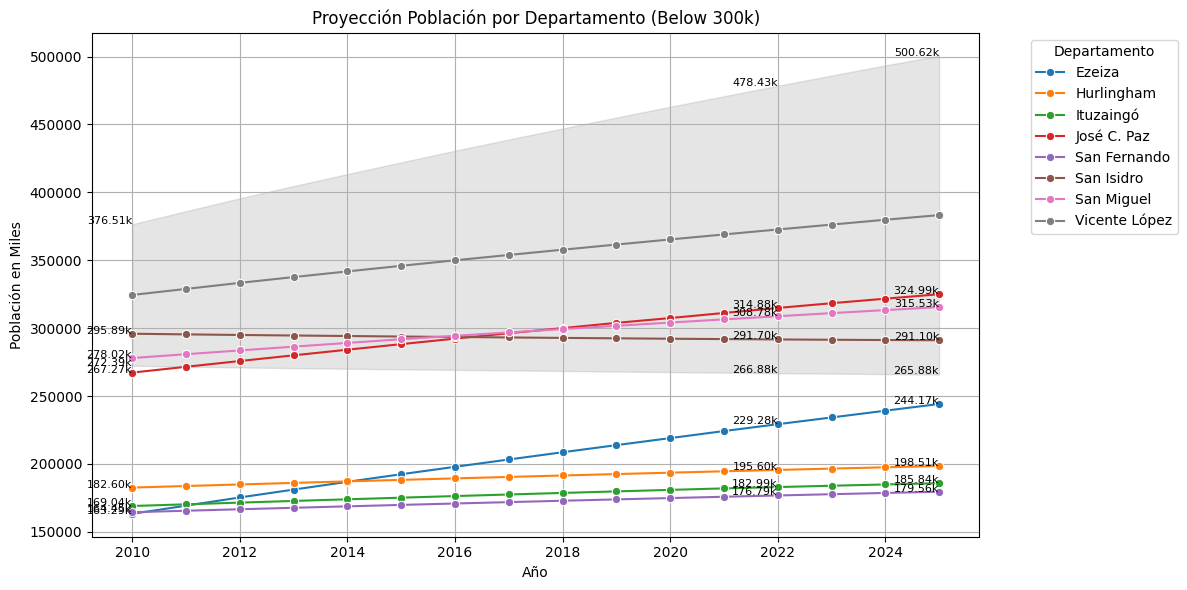
\includegraphics[width=0.8\textwidth]{{C:/Users/Fer/ITBA_TFI/code/latex/img/ProyLineas300k.png}}
  \caption{Población por departamento 2010-2025.INDEC}
  \label{fig:proy300k}
\end{figure}

\begin{figure}[htbp]
  \centering
  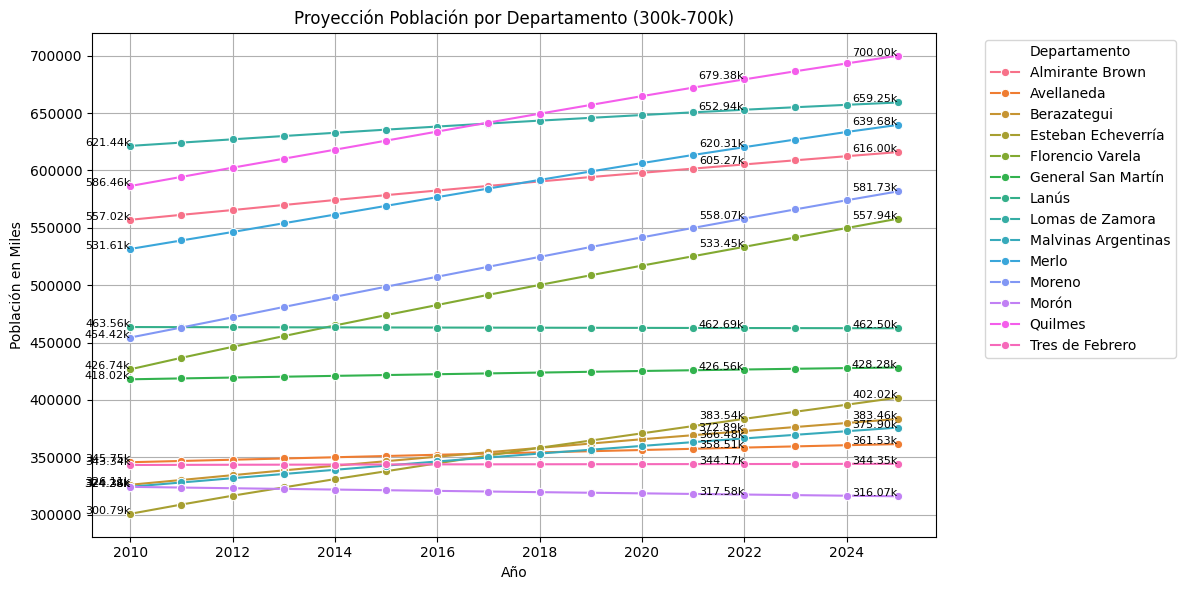
\includegraphics[width=0.8\textwidth]{{C:/Users/Fer/ITBA_TFI/code/latex/img/ProyLineas700k.png}}
  \caption{Población por departamento 2010-2025.INDEC}
  \label{fig:proy700k}
\end{figure}
\begin{figure}[htbp]
  \centering
  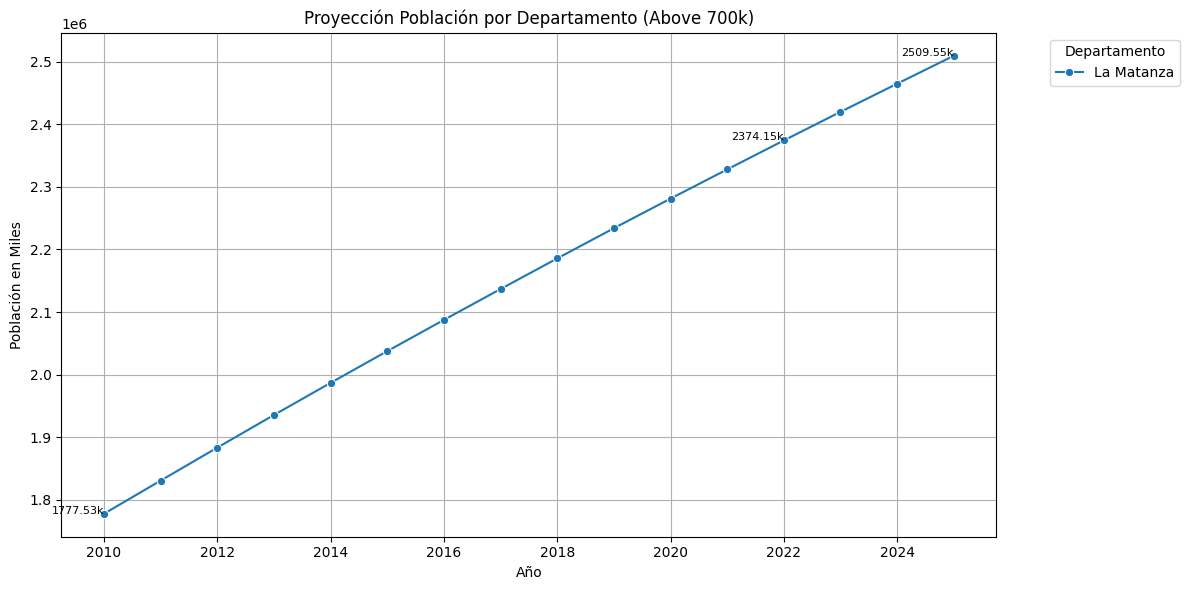
\includegraphics[width=0.8\textwidth]{{C:/Users/Fer/ITBA_TFI/code/latex/img/ProyLineas1.300k.png}}
  \caption{Población por departamento 2010-2025.INDEC}
  \label{fig:proyMayor700k}
\end{figure}

\subsection{Componente Geográfico }
Con el objetivo de enriquecer el dataset se incorpora una tabla con los polígonos georeferenciados corespondientes a cada departamento.
 La misma se obtiene a través de capa SIG de todos los departamentos de la República Argentinadel del Instituto Geográfico Nacional  \customcite{IGMSig}. 
Luego, dichos datos se cruzan con el listado de departamentos del AMBA, generando un dataset enriquecido con las caracteristicas geográficas, que completan 
los datos censales recopilados desde 1991 a 2022. La capa geográfica incorpora las variables que se detallan en el Cuadro \ref{tab:geo.depto}.
%Descripción de Variables Geográficas
\begin{table}[htbp]
    \centering
    \begin{tabular}{|l|l|p{8cm}|}
        \hline
        \textbf{Variable} & \textbf{Nombre} & \textbf{Descripción} \\
        \hline
        geom & geometry & Polígono WKT con los límites del departamento \\
        fna & Nombre geográfico & Nombre completo que se utiliza para designar un objeto en un mapa o carta. Está formado por el término genérico y el término específico. Ejemplo: río Mendoza. \\
        gna & Término genérico & Parte del nombre geográfico que indica el tipo de objeto que identifica. Ejemplo: río, monte, glaciar, establecimiento. \\
        nam & Término específico & Parte de un nombre geográfico que acompaña al término genérico y que identifica e individualiza un objeto geográfico determinado. Ejemplo: Paraná en río Paraná; Upsala en glaciar Upsala; Las Marías en establecimiento Las Marías; Esperanza en el caso de bahía Esperanza. \\
        in1 & Código INDEC & Código único de vías de circulación asignado por el Instituto Nacional de Estadística y Censos de la República Argentina. \\
        fdc & Fuente de captura & Identificación del nombre y tipo de fuente utilizada para capturar la información. Puede incluir fecha y otros datos adicionales. \\
        sag & Autoridad de fuente & Nombre de la autoridad responsable de la información utilizada. \\
        \hline
    \end{tabular}
  \caption{Descripción de Variables Geográficas}
    \label{tab:geo.depto}
\end{table}


\subsection{Población}
Se detallan a continuación los datos recopilados 
según nivel de agregación.En primera instancia se  generó un dataset con todos los departamentos del AMBA,
 sus caracteristicas georgráficas,así como los valores
de las variables censales correspondientes a los censos 1991-2001-2010-2022.En el cuadro \ref{tab:censos_amba} 
se puede observar el esquema del dataset.
%CENSOS AMBA
\begin{table}[htb]
  \centering
  \footnotesize
  \begin{tabular}{|c|c|c|c|c|c|c|c|c|c|c|}
  \hline
    \textbf{\cellcolor[rgb]{0,0.231,0.427}\textcolor{white}{nam}} &
   \textbf{\cellcolor[rgb]{0,0.231,0.427}\textcolor{white}{$cod_depto$}} 
   & \textbf{\cellcolor[rgb]{0,0.231,0.427}\textcolor{white}{anio}} &
   \textbf{\cellcolor[rgb]{0,0.231,0.427}\textcolor{white}{pob}} & 
   \textbf{\cellcolor[rgb]{0,0.231,0.427}\textcolor{white}{var}} & 
   \textbf{\cellcolor[rgb]{0,0.231,0.427}\textcolor{white}{muj}} &
    \textbf{\cellcolor[rgb]{0,0.231,0.427}\textcolor{white}{vivpart}} & 
    \textbf{\cellcolor[rgb]{0,0.231,0.427}\textcolor{white}{vivtotal}} &
     \textbf{\cellcolor[rgb]{0,0.231,0.427}\textcolor{white}{sup}} &
      \textbf{\cellcolor[rgb]{0,0.231,0.427}\textcolor{white}{$ind_masc$}} &
       \textbf{\cellcolor[rgb]{0,0.231,0.427}\textcolor{white}{$dens_pob$}} \\
  \hline
  Almirante Brown & 06028 & 1991 & 450698.0 & 222042.0 & 228656.0 & nan & nan & 157.87 & 97.1 & 2854.87 \\
  Almirante Brown & 06028 & 2001 & 515556.0 & 252454.0 & 263102.0 & 143543.0 & 88.0 & 157.87 & 96.0 & 3265.70 \\
  Almirante Brown & 06028 & 2010 & 552902.0 & 270247.0 & 282655.0 & 156218.0 & 78.0 & 157.87 & 95.6 & 3502.26 \\
   Almirante Brown & 06028 & 2022 & 585852.0 & 281842.0 & 301779.0 & 184403.0 & 60.0 & 157.87 & 93.4 & 3710.98 \\
    Avellaneda & 06035 & 1991 & 344991.0 & 164243.0 & 180748.0 & nan & nan & 68.54 & 90.9 & 5033.43 \\
  Avellaneda & 06035 & 2001 & 328980.0 & 155450.0 & 173530.0 & 117200.0 & 59.0 & 68.54 & 89.6 & 4799.82 \\
  Avellaneda & 06035 & 2010 & 342677.0 & 162264.0 & 180413.0 & 121307.0 & 68.0 & 68.54 & 89.9 & 4999.66 \\
  Avellaneda & 06035 & 2022 & 370939.0 & 174572.0 & 194911.0 & 144988.0 & 64.0 & 68.54 & 89.6 & 5412.01 \\
  ...... &  &  &  &  &  & &  &  &  &  \\ \hline
  \end{tabular}
  \caption{Dataset Censos AMBA}
  \label{tab:censos_amba}
  \end{table}
  
  En el Cuadro \ref{tab:summaryCensos} se muestra una agregación de todos los campos del dataset a nivel global. 
  En el mismo, podemos notar que para os campos correspondientes a población (pob, var, muj, ind\_masc, dens\_pob) 
  hay una cantidad menor de valores, debido al hecho de los valores nulos que se corresponden con los casos de municipios 
  que han desaparecido en la reorganización administrativa desde 1991 a 2001, a saber: Esteban Echeverría, Ezeiza,Florencio Varela, 
  Hurlingham, Ituzaingó, José C. Paz, Malvinas Argentinas, Morón,San Miguel y General Sarmiento. \\
  También hay una pérdida de registros vivpart y vivtotal, dado que para el censo 1991 no se detalla el total de viviendas particules y colectivas.

  %summaryCensos
\begin{table}[htb]
    \centering
    \begin{tabular}{llll}
        \toprule
        \textbf{Column} & \textbf{Non-Null Count} & \textbf{Dtype} \\
        \midrule
        nam & 96 & object \\
        cod\_depto & 96 & object \\
        anio & 96 & object \\
        pob & 90 & float64 \\
        var & 90 & float64 \\
        muj & 90 & float64 \\
        vivpart & 72 & float64 \\
        vivtotal & 72 & float64 \\
        sup & 96 & object \\
        ind\_masc & 90 & object \\
        dens\_pob & 90 & object \\
        \bottomrule
    \end{tabular}
  \caption{Resumen de columnas de Censos AMBA}
    \label{tab:summaryCensos}
\end{table}

\subsubsection{Población: Geolocalización}

En este caso se ofrece una visualización geográfica del dataset. Utilizando el sofware QGIS conectado directamente a la base de 
datos AMBA (POSTGRES) se pudo disponer la información de cada Departamento con su geolocalización.
Se detalla en la Figura \ref{fig:AllPob} la poblacion total para cada departamento (Censos 1991-2022), donde se observa claramente que el distrito más poblado
es La Matanza.

%%% QGIS GRAPHICS
\begin{landscape}
\begin{figure}[p] % Use 'p' to force the figures to be placed on a separate page
  \centering
  \begin{subfigure}[b]{0.48\textwidth}
      \centering
      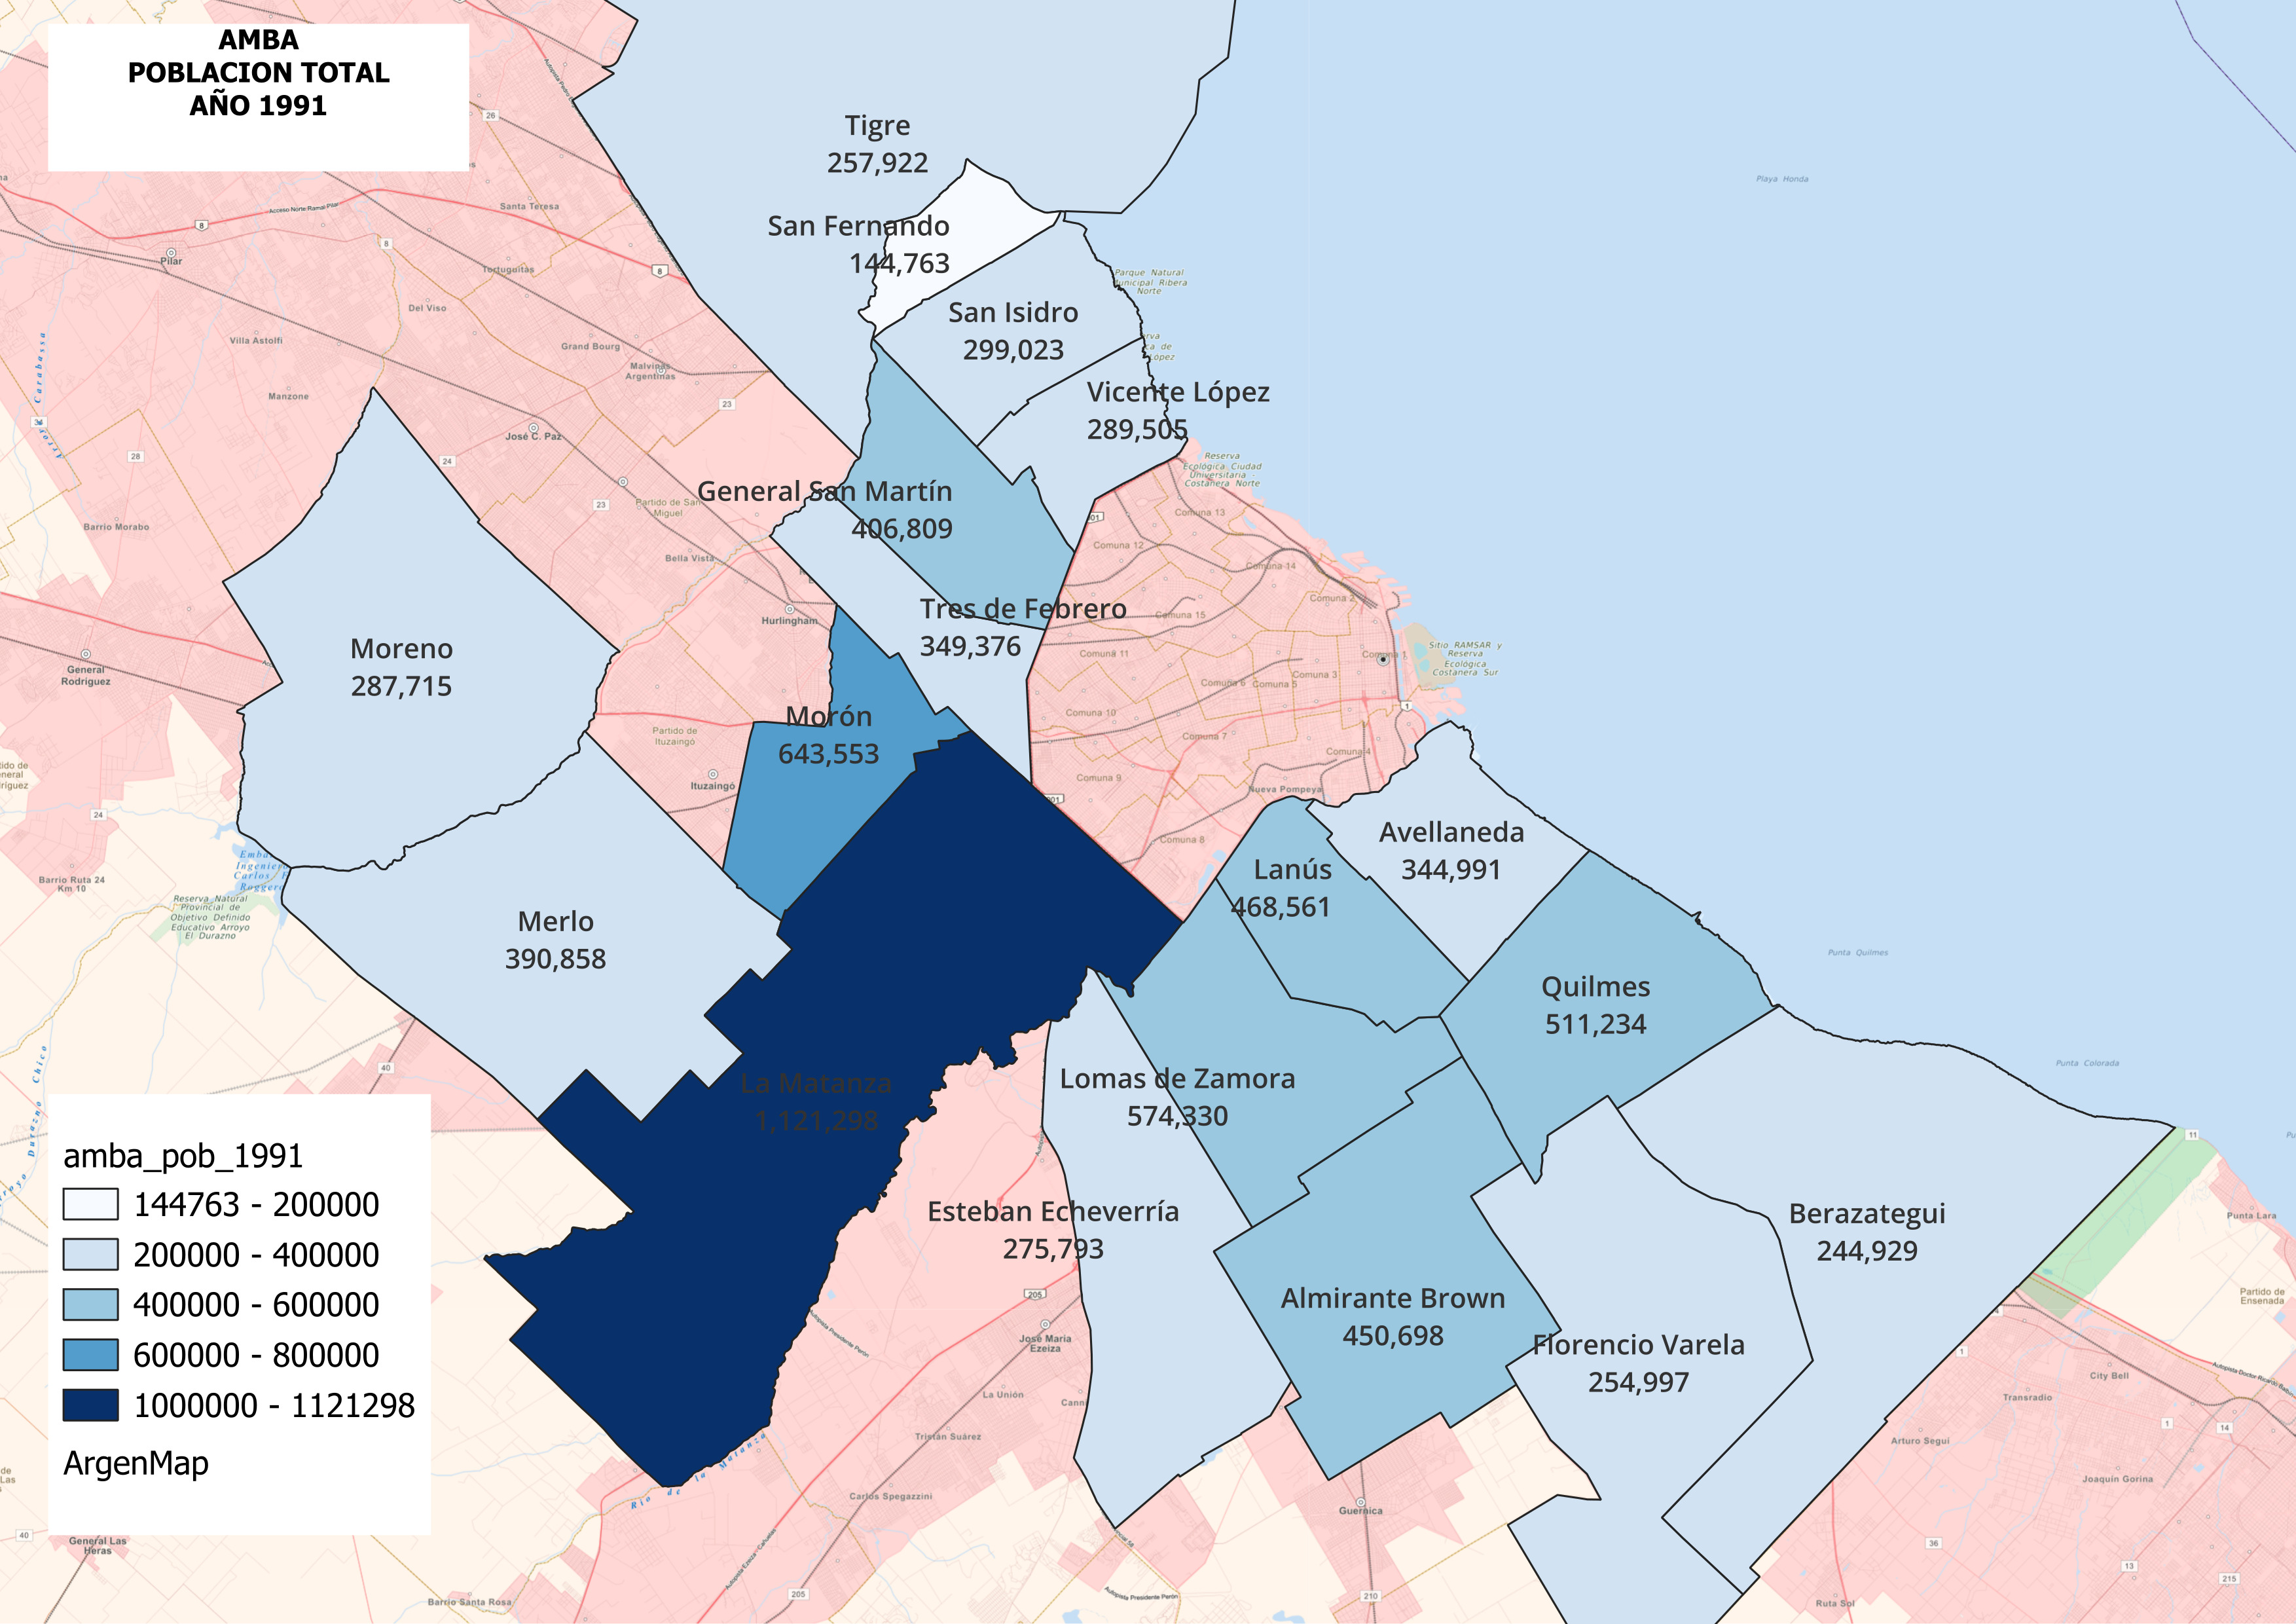
\includegraphics[width=\textwidth]{{C:/Users/Fer/ITBA_TFI/QGIS/img/AmbaPob1991.jpg}}
      \caption{AMBA- Población total Censo 1991}
      \label{fig:pob1991}
  \end{subfigure}
  \quad % Add some horizontal space between subfigures
  \begin{subfigure}[b]{0.48\textwidth}
      \centering
      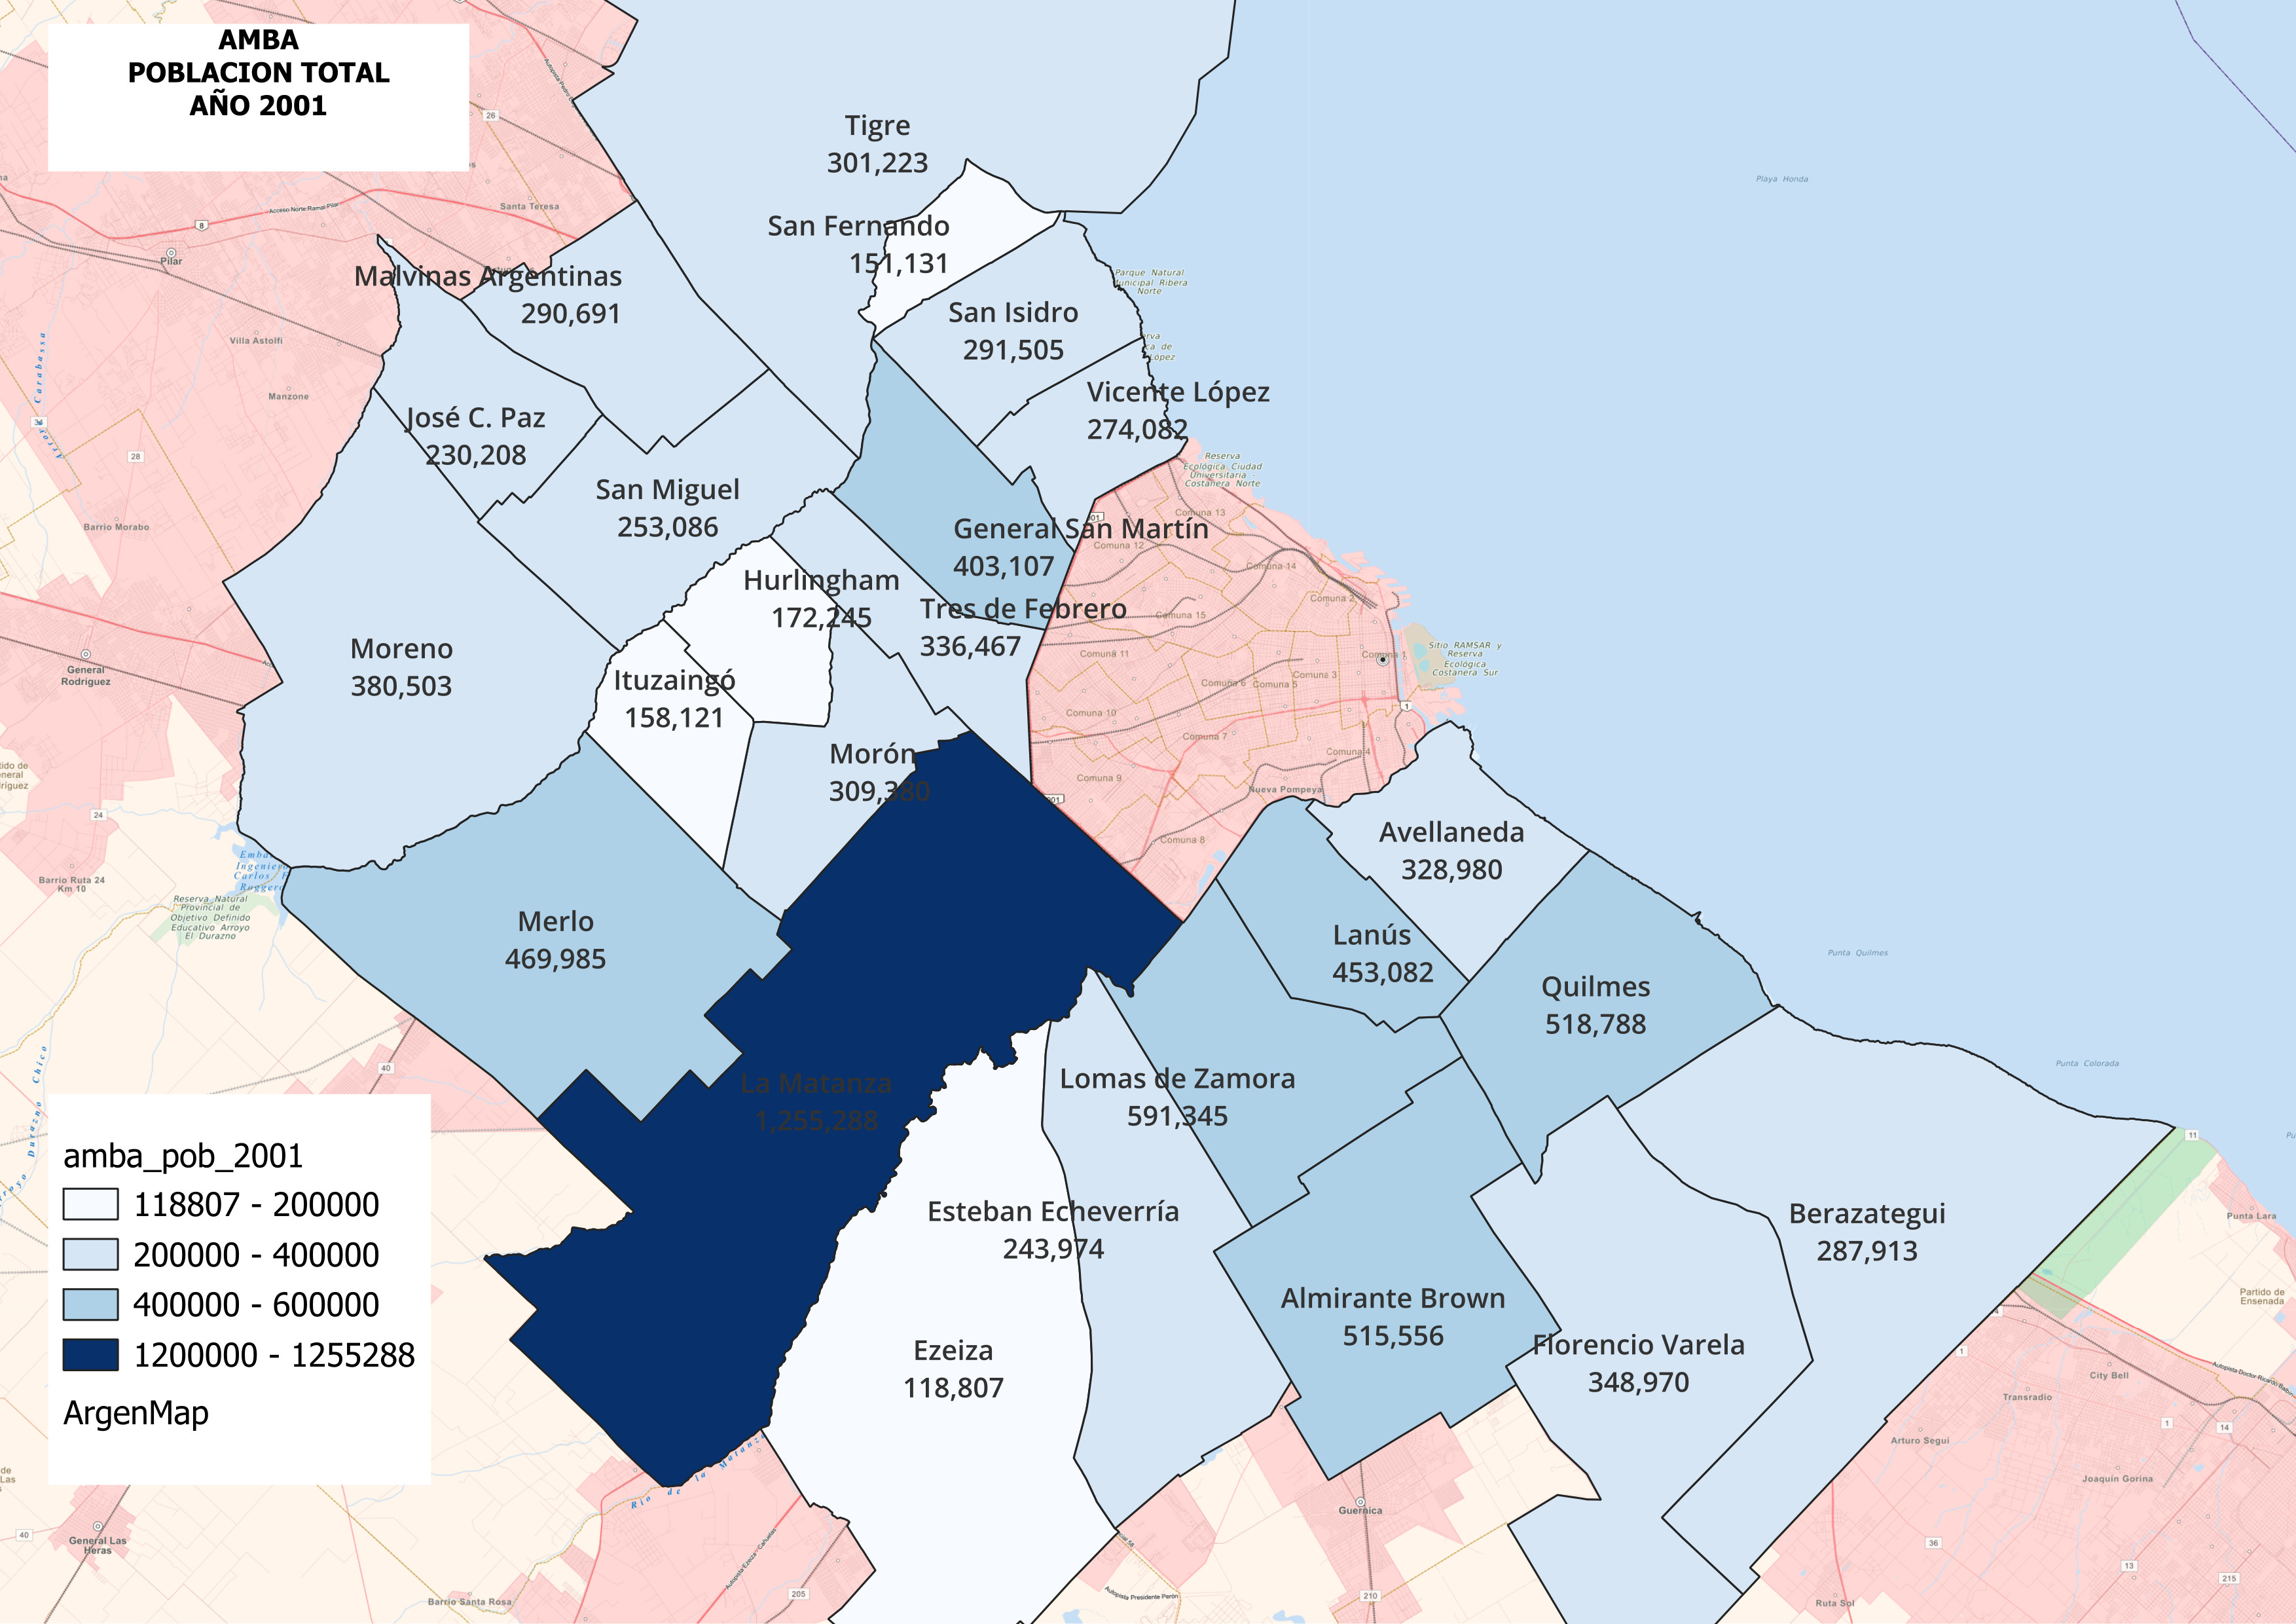
\includegraphics[width=\textwidth]{{C:/Users/Fer/ITBA_TFI/QGIS/img/AmbaPob2001.jpg}}
      \caption{AMBA- Población total Censo  2001}
      \label{fig:pob2001}
  \end{subfigure}
  
  \begin{subfigure}[b]{0.48\textwidth}
      \centering
      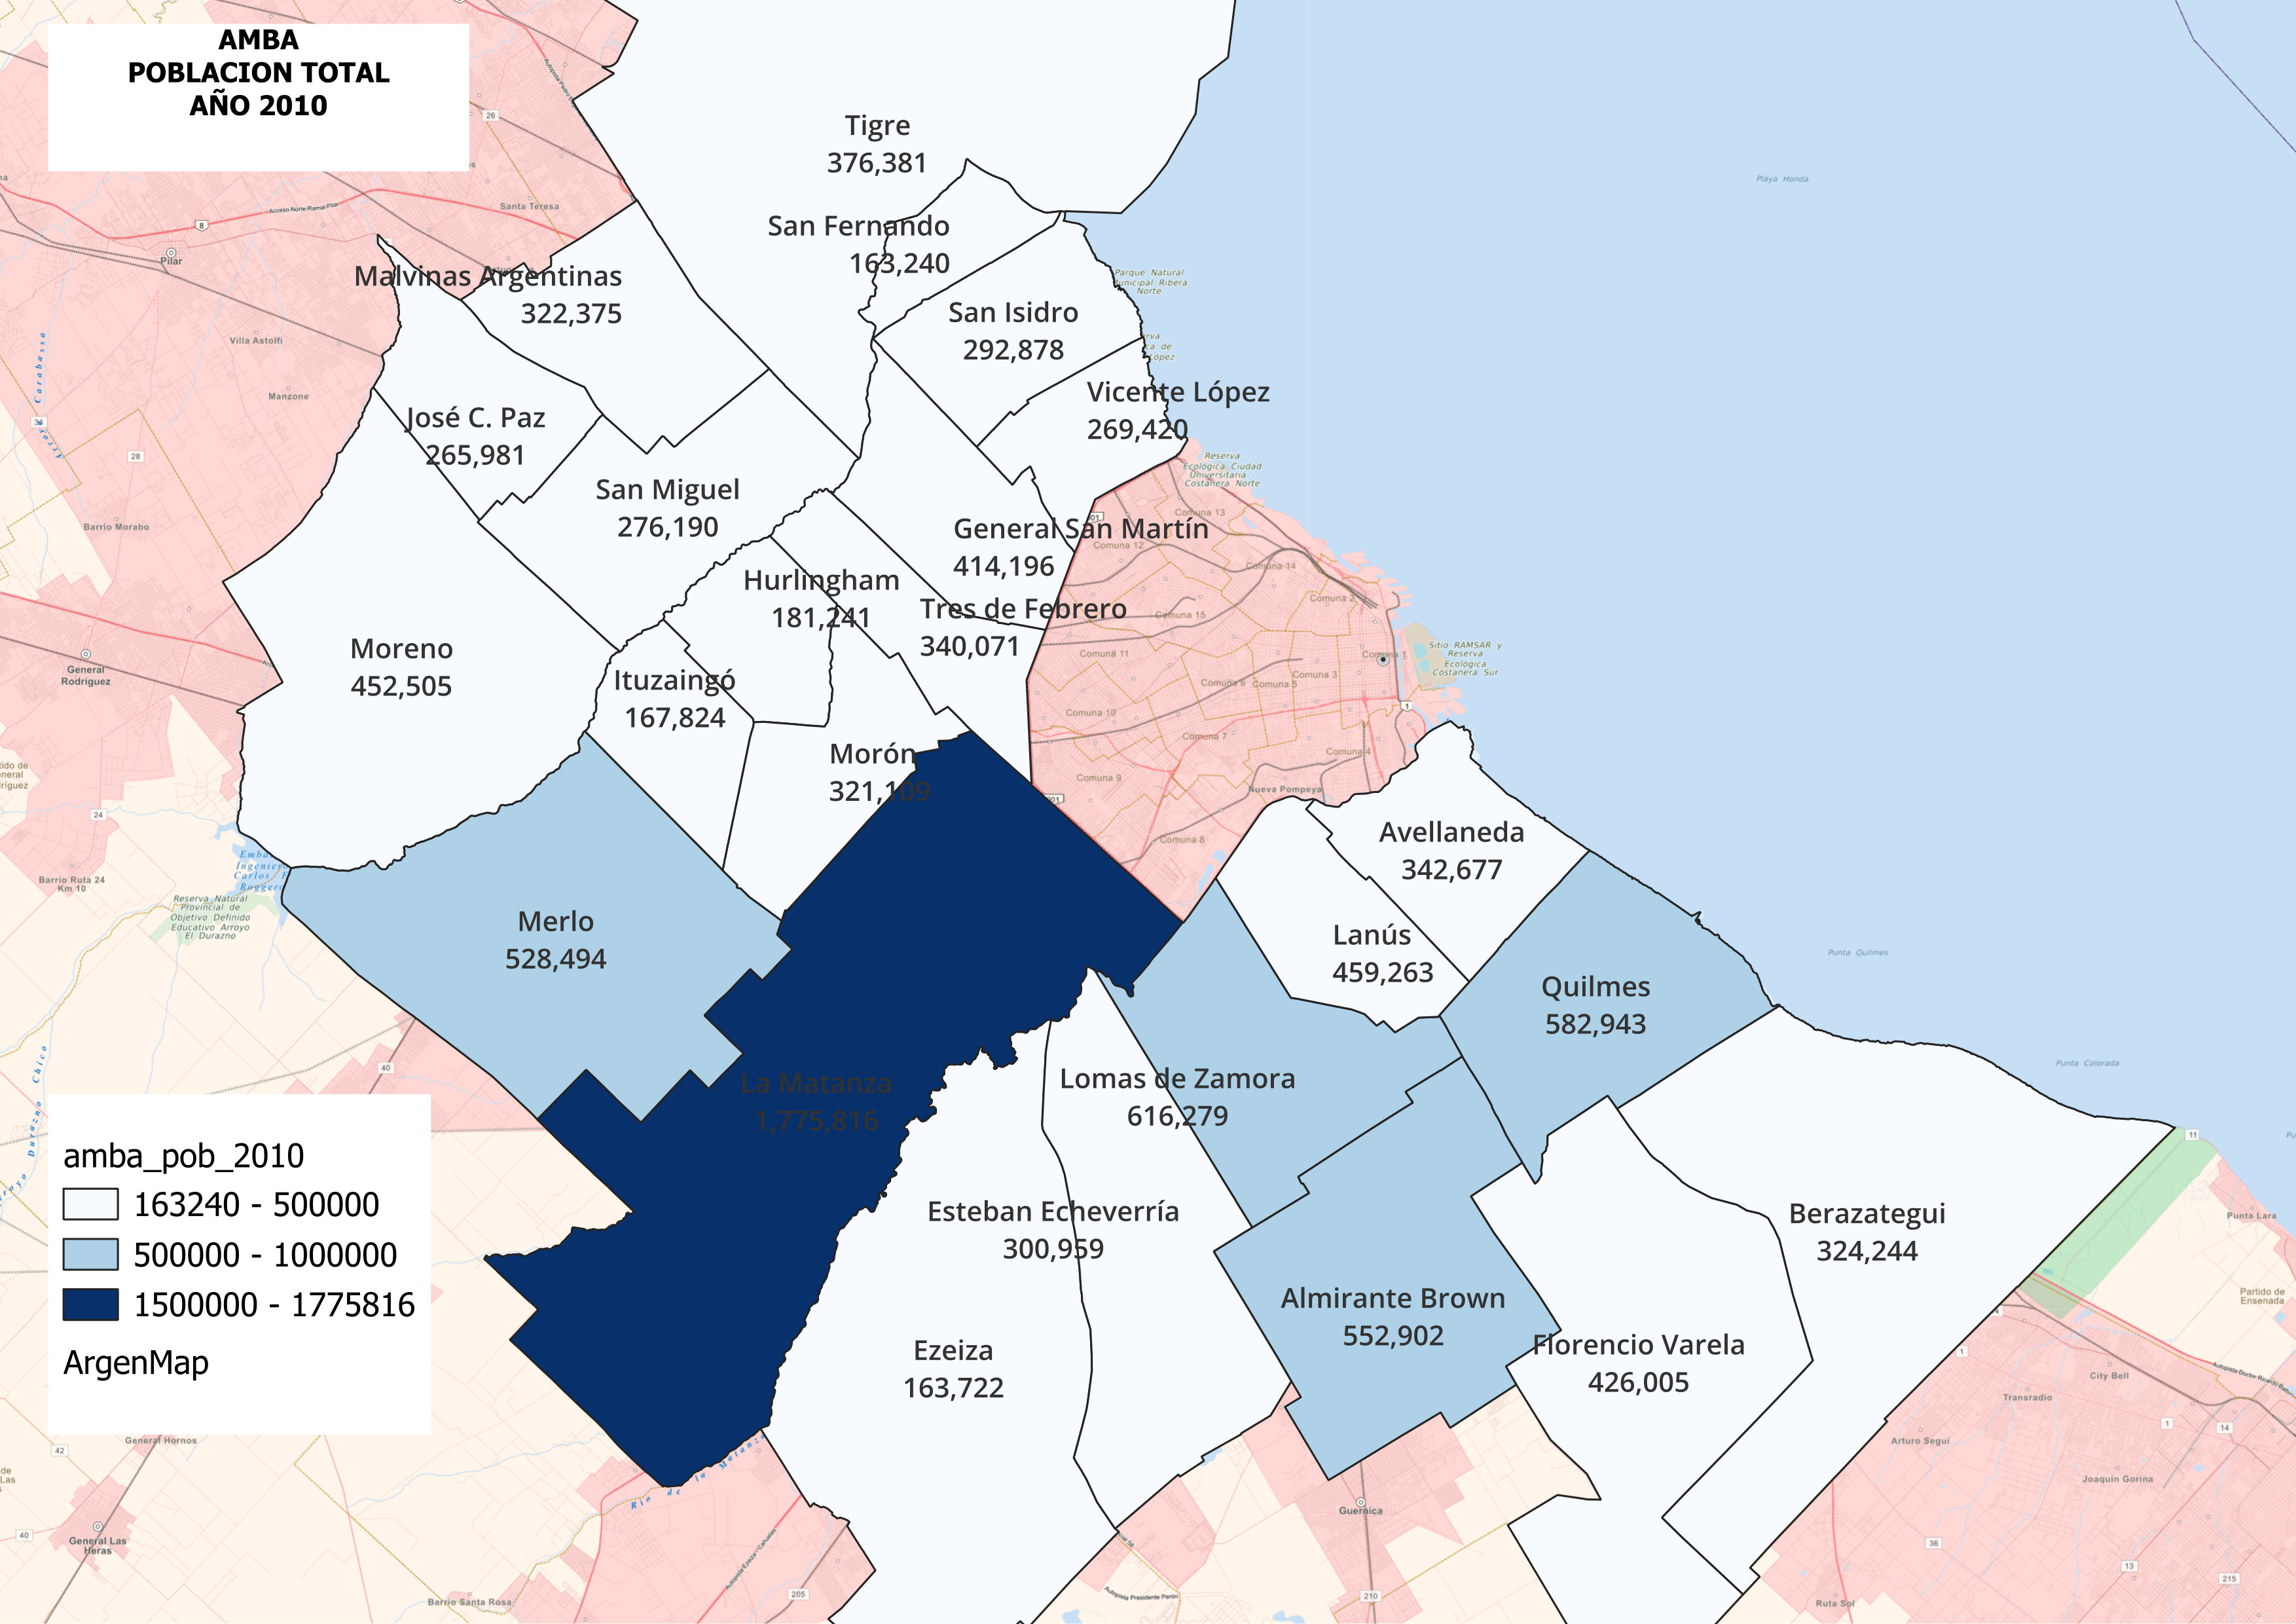
\includegraphics[width=\textwidth]{{C:/Users/Fer/ITBA_TFI/QGIS/img/AmbaPob2010.jpg}}
      \caption{AMBA- Población total Censo 2010}
      \label{fig:pob2010}
  \end{subfigure}
  \quad % Add some horizontal space between subfigures
  \begin{subfigure}[b]{0.48\textwidth}
      \centering
      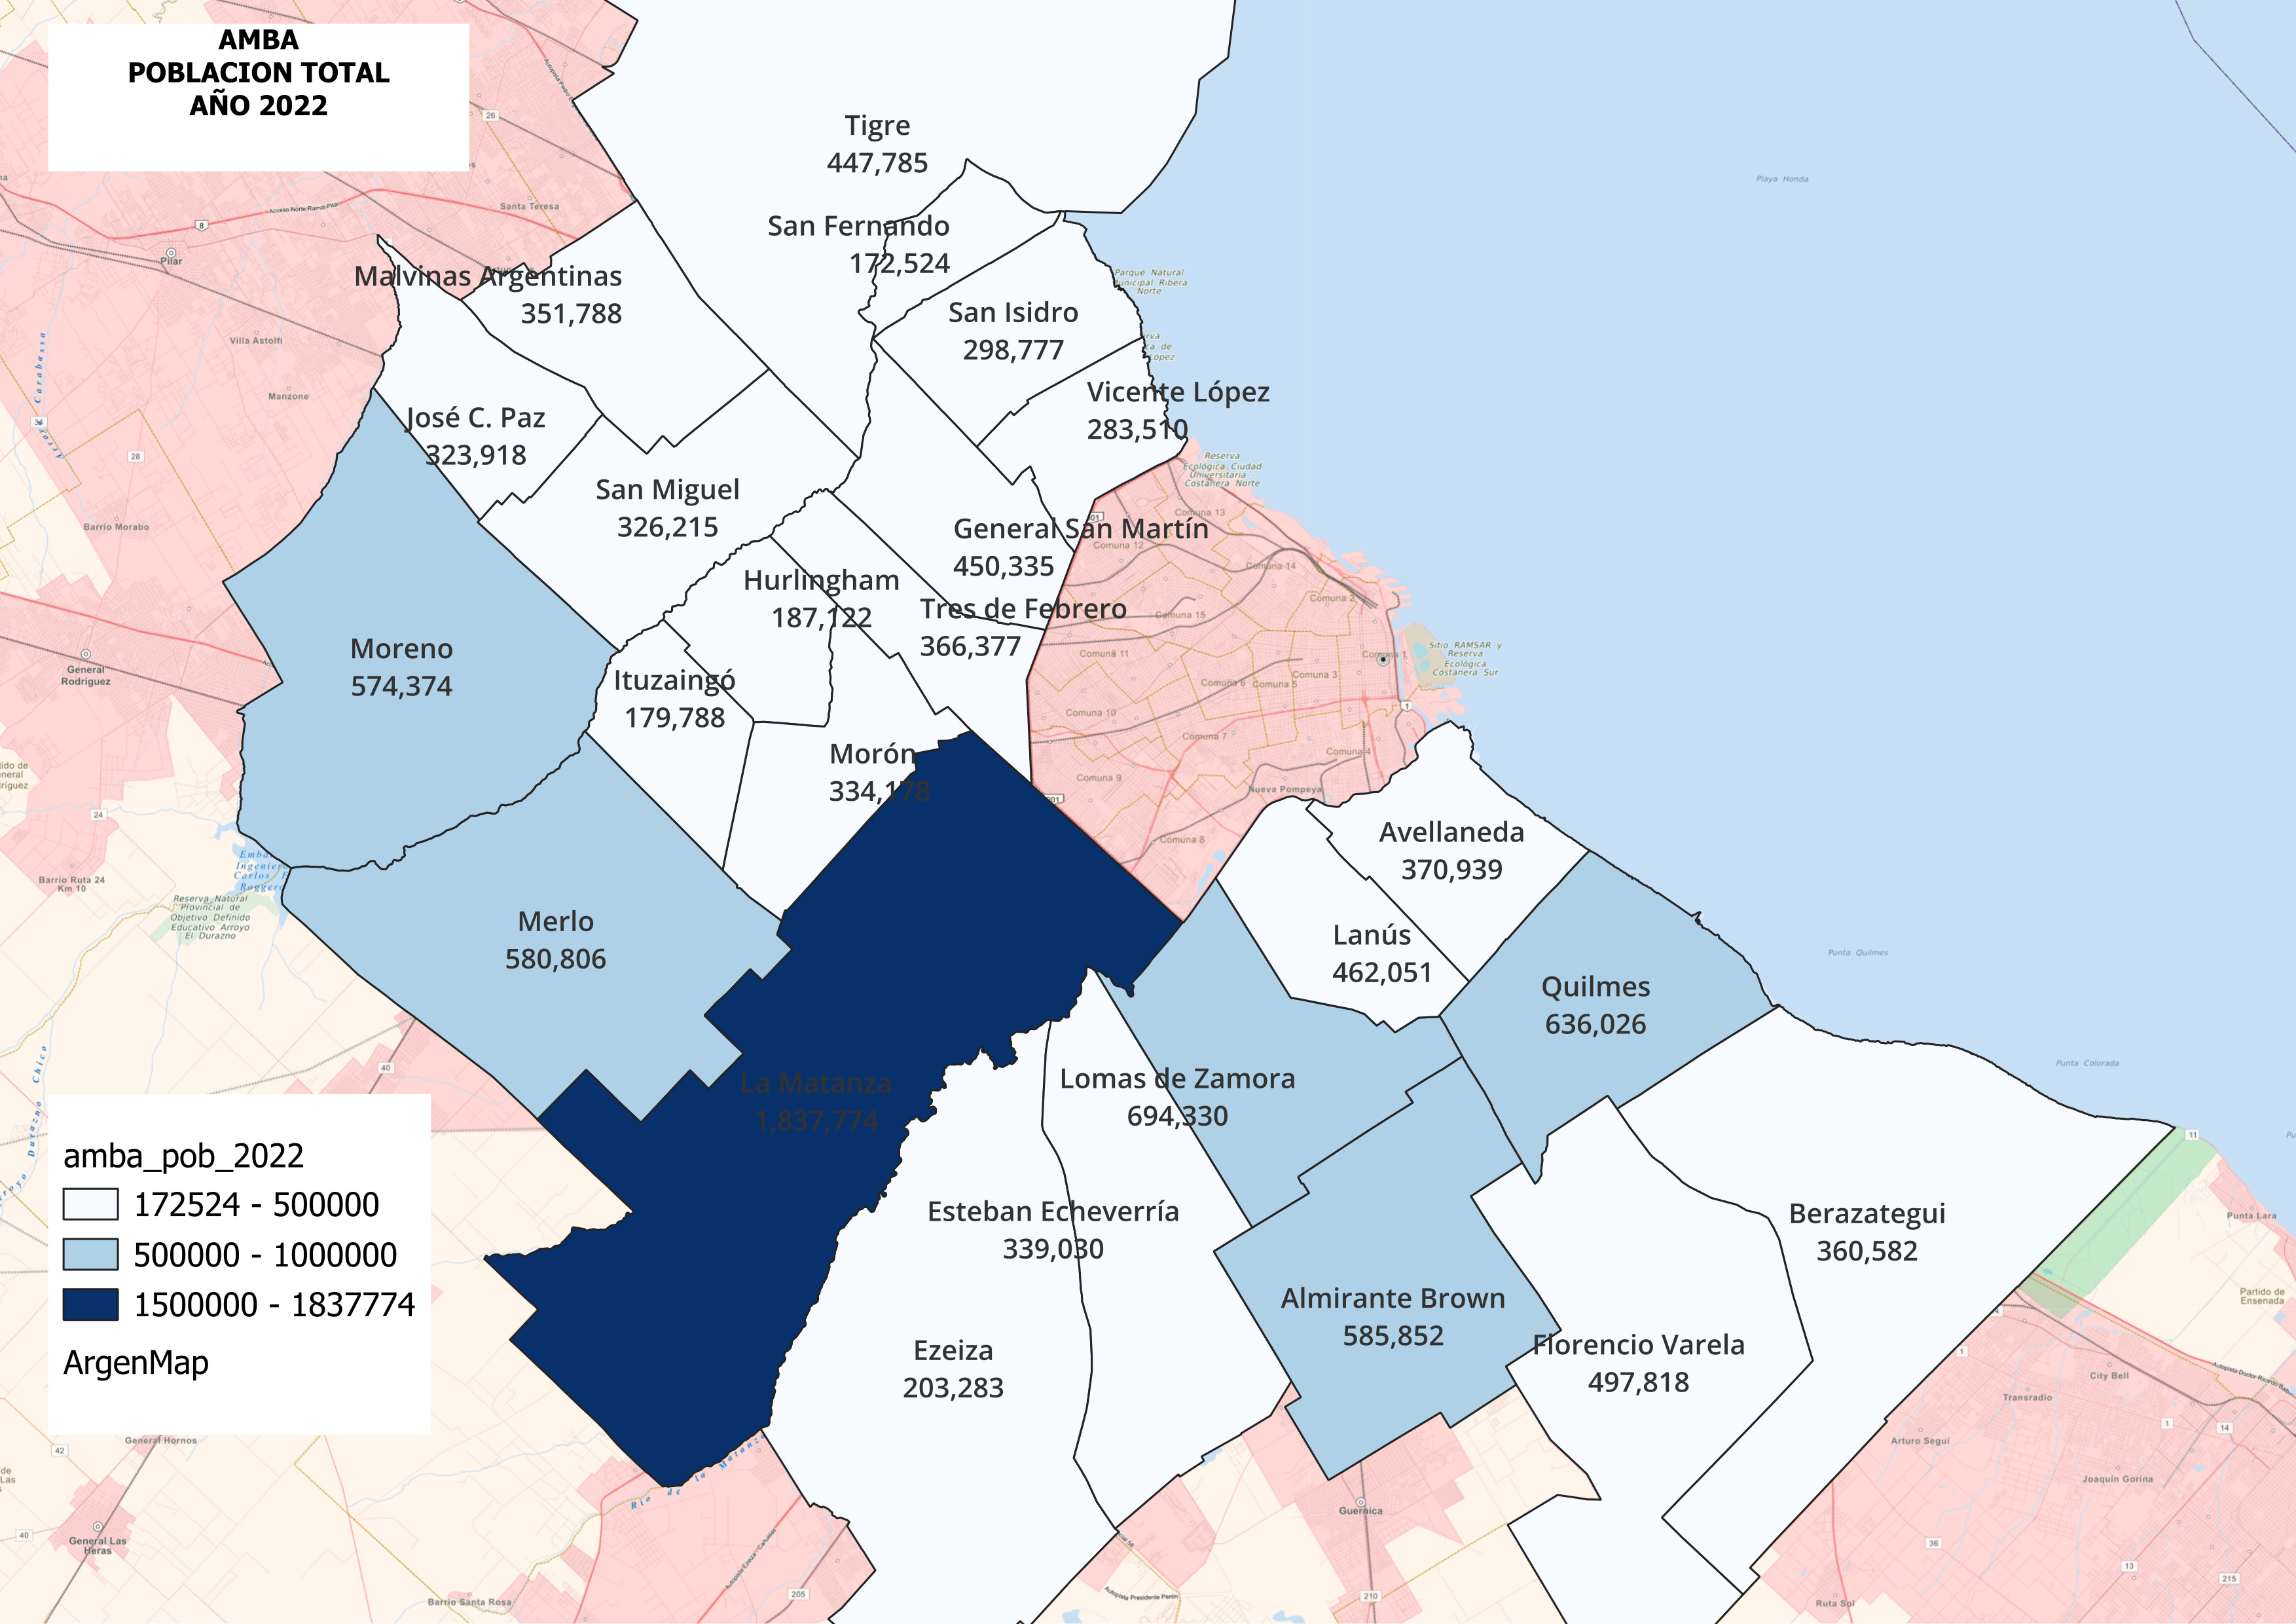
\includegraphics[width=\textwidth]{{C:/Users/Fer/ITBA_TFI/QGIS/img/AmbaPob2022.jpg}}
      \caption{AMBA- Población total Censo 2022}
  \label{fig:pob2022}
  \end{subfigure}
  \caption{Población Total Censos 1991-2022}
\label{fig:AllPob}
\end{figure}
\end{landscape}


\subsubsection{Tasa de Crecimento en Población}
  Se determinaron los ratios de crecimento entre censos consecutivos para cada departamento.
  Para este análisis se trató de manera difrenciada aquellos municipios que han sufrido modificaciones administrativas
  desde 1991  a 2001: \textbf{Esteban Echeverría, Ezeiza, Florencio Varela, Hurlingham, Ituzaingó, José C. Paz,Malvinas Argentinas, 
Morón, San Miguel y General Sarmiento}. En los mismos, al desmembrarse en varios partidos, resignando superficie, algunas tasas o ratios de crecimiento 
  se muestran negativos. Asimismo, los partidos que han visto incrementada su superfice, presentan tasas de crecimiento no representativas del 
  fenómeno demográfico.\newline\newline
  Por otra parte, los partidos que desaparecen o se crean en el año 2001 no se consideran en el valor del ratio para el intervalo 1991-2001.\newline\newline
    En el Cuadro \ref{tab:RatiosAll} se pueden observar un fragmento de los valores obtenidos. Para el año en cuestion la tasa surge de dividir el valor poblacional
  del censo de este año sobre el valor poblacional del censo anterior, expresado en porcentaje.\newline\newline
  Es decir: 
  \begin{equation}
    \underset{\text{\footnotesize(Año $X$)}}{\text{Growth Ratio}} = 
    \left( \frac{\underset{\text{\footnotesize(Censo $X$)}}{\text{Población}}}{\underset{\text{\footnotesize(Censo $X-1$)}}{\text{Población}}} - 1 \right) \times 100
  \end{equation}

  \begin{table}[htb]
    \centering
    \begin{tabular}{|c|c|c|c|}
    \hline
    \textbf{\cellcolor[rgb]{0,0.231,0.427}\textcolor{white}{nam}} &
     \textbf{\cellcolor[rgb]{0,0.231,0.427}\textcolor{white}{anio}}
      & \textbf{\cellcolor[rgb]{0,0.231,0.427}\textcolor{white}{pob}}
       & \textbf{\cellcolor[rgb]{0,0.231,0.427}\textcolor{white}{growth\_ratio}} \\ \hline
    Almirante Brown & 2001 & 515556.0 & 14.39 \\
    Almirante Brown & 2010 & 552902.0 & 7.24 \\
    Almirante Brown & 2022 & 585852.0 & 5.96 \\
    Avellaneda & 2001 & 328980.0 & -4.64 \\
    Avellaneda & 2010 & 342677.0 & 4.16 \\
    Avellaneda & 2022 & 370939.0 & 8.25 \\
    Berazategui & 2001 & 287913.0 & 17.55 \\
    Berazategui & 2010 & 324244.0 & 12.62 \\
    Berazategui & 2022 & 360582.0 & 11.21 \\
    Esteban Echeverría & 2001 & 243974.0 & -11.54 \\
    Esteban Echeverría & 2010 & 300959.0 & 23.36 \\
    Esteban Echeverría & 2022 & 339030.0 & 12.65 \\
      ....& & & \\
  
    \hline
    \end{tabular}
    \caption{Extracto: Tasa de crecimiento Intercensal}
  \label{tab:RatiosAll}
    \end{table}
  

    A partir de un análisis estadísitico simple sobre estas tasas decrecimiento, en el Cuadro \ref{tab:summary_growth_ratio} 
    podemos observar una gran disparidad en los valores, a pesar de que se trata de un sector geográfico de similares características socio-demográficas. 
\begin{table}[htbp]
    \centering
    \begin{tabular}{lr}
        \hline
        \textbf{Estadístico} & \textbf{Valor} \\
        \hline
        Count & 66\\
        Mean & 9.3 \\
        Standard Deviation & 13.1 \\
        Minimum & -51.9 \\
        25\% Percentile & 3.0 \\
        50\% Percentile & 8.1\\
        75\% Percentile & 16.5 \\
        Maximum & 41.5 \\
        \hline
    \end{tabular}
    \caption{Resumen Estadísitco de Tasas de Crecimiento}
    \label{tab:summary_growth_ratio}
\end{table}
\newline\newline

A partir de la elaboración de un gráfico boxplot se determinaron los Outliers para estas tasas de crecimiento. En la Figura \ref{fig:boxplotRatios}
se pueden observar cuatro outliers, tanto en valores positivos como negativos. Como se comentó anteriormente no se analizarán los casos con modificaciones administrativas desde 1991 a 2001.
En el Cuadro \ref{tab:DimDepto} se detallan los cuatro outliers para estas tasas de crecimiento intercensal.  Una vez desestimado el caso de Morón para el período 1991-2001 donde la tasa es negativa de 51.9\%, 
debido a la cesión de tierras para la creación de distintos partidos, en la Figura \ref{fig:OutlierlineasPob}, se puede ver la curva población de los 3 outiliers destacados: Florencio Varela ,La Matanza y Ezeiza.\newline\newline

\begin{figure}[htbp]
  \centering
  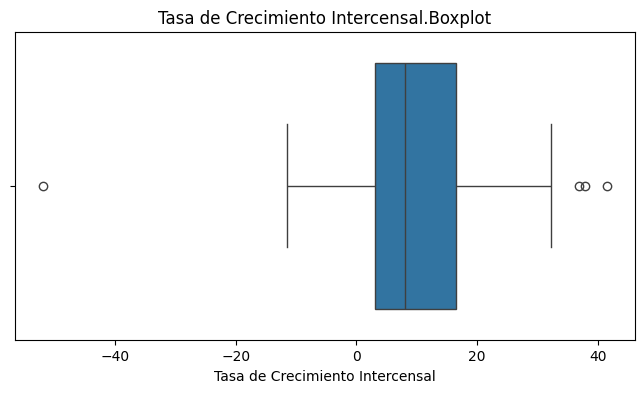
\includegraphics[width=0.8\textwidth]{{C:/Users/Fer/ITBA_TFI/code/latex/img/GrowthRatioBoxplot.png}}
  \caption{Box plot Tasas de crecmiento intercensal 1991-2022}
  \label{fig:boxplotRatios}
\end{figure}

\begin{table}[htbp]
  \centering
  \begin{tabular}{|c|c|c|c|r|r|}
      \hline
      \textbf{id} & \textbf{nam} & \textbf{codDepto} & \textbf{anio} & \textbf{pob} & \textbf{growthRatio} \\
      \hline
      54 & Morón & 06568 & 2001 & 309380.0 & -51.92 \\
      78 & Florencio Varela & 06274 & 2001 & 348970.0 & 36.85 \\
      13 & La Matanza & 06427 & 2010 & 1775816.0 & 41.47\\
      29 & Ezeiza & 06270 & 2010 & 163722.0 & 37.80 \\
      \hline
  \end{tabular}
  \caption{Outliers para Tasas de crecmiento intercensal}
\label{tab:RatiosOutliers}
\end{table}


\begin{figure}[htbp]
  \centering
  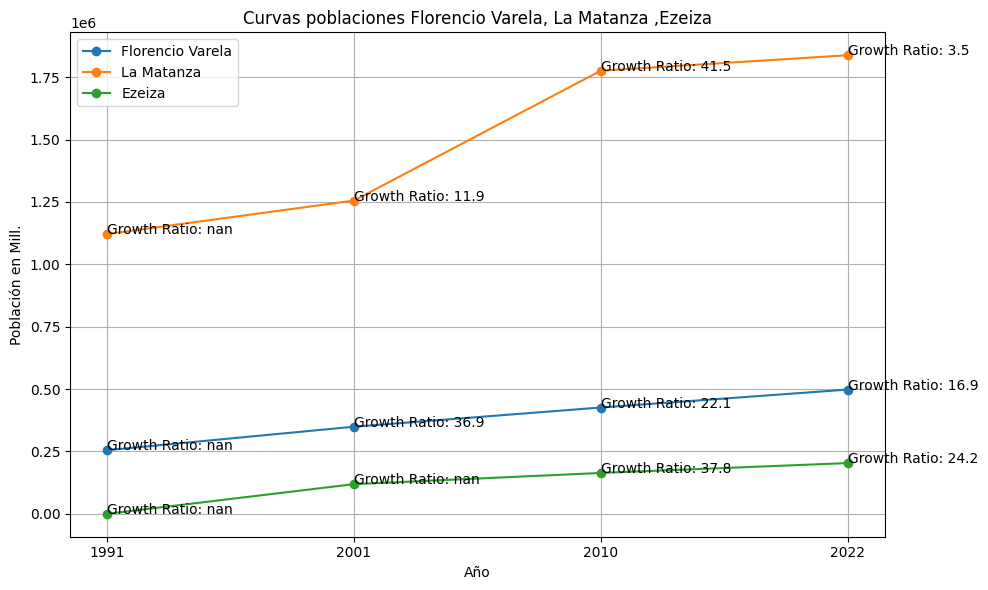
\includegraphics[width=0.8\textwidth]{{C:/Users/Fer/ITBA_TFI/code/latex/img/CurvasOutliersRatios.png}}
  \caption{Curvas de Población por Departamento 1991-2022}
    \label{fig:OutlierlineasPob}
\end{figure}


\subsubsection{Tasas de Crecimento Intercensal: Coeficiente de Variación}

Con el objetivo de profundizar el análsis de las tasas de crecimiento, se procedió a calcular la variación en la tasa de crecimiento por Departamento.\newline\newline
Sobre la media y la desviación estándar de cada subset de datos, se define el coeficiente de variación (CV) como:

\begin{equation}
  \underset{\text{\footnotesize(Departametno)}}{\text{CV}} = 
  \left( \frac{\underset{\text{\footnotesize(Departamento)}}{\text{Std.Dev}}}{\underset{\text{\footnotesize(Departamento)}}{\text{Mean}}} \right) \times 100
\end{equation}

El coeficiente de variación es una medidad de la dispersión alrededor de la media de la población. En este caso, vemos curvas poblacionales
con gran dispersión en su tasas de crecimento para los censos del periodo analizado año 1991-2022. \newline\newline

En la Figura \ref{fig:CVOutliersPoblacion} se observa el resultado. Se destaca en particular los valores extremos
tanto negativos como positivos, a saber : Vincente López, Morón, Tres de Febrero, Avellaneda, La Matanza, Esteban Echeverría y General San Martín.  
\newline\newline 

Cabe recordar en este instancia que, los partidos de Esteban Echeverría, Florencio Varela y Morón sufrieron modificaciones administrativa en el período 1991-2001.
 En la Figuras \ref{fig:CVoutCurvasMedia} y \ref{fig:CVoutCurvasAlta} pueden observarse las curvas poblacionales de los mencionados departamentos destacados, difreenciadas para 
población media y alta, respectivamente.\newline\newline
En estos casos se prestará particular atención a las predicciones hechas por el INDEC, así como las metodologías que se implementen 
para la estimación de la curva poblacional, ya que es esperable un mayor error de predicción en estos departamentos cuyas curvas presentan singularidades respecto a
los municipios inmediatamente aledaños.


\begin{figure}[htbp]
  \centering
  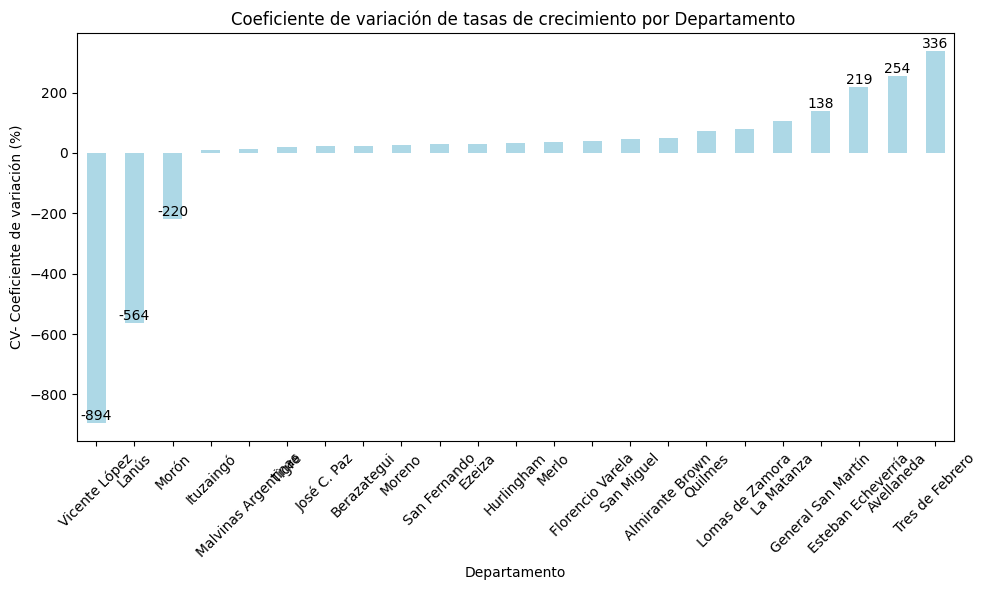
\includegraphics[width=0.8\textwidth]{{C:/Users/Fer/ITBA_TFI/code/latex/img/CVGrowthRatioAll.png}}
  \caption{CV.Coeficiente de variación por departamento -1991-2022}
\label{fig:CVOutliersPoblacion}
\end{figure}

 
\begin{figure}[htbp]
  \centering
  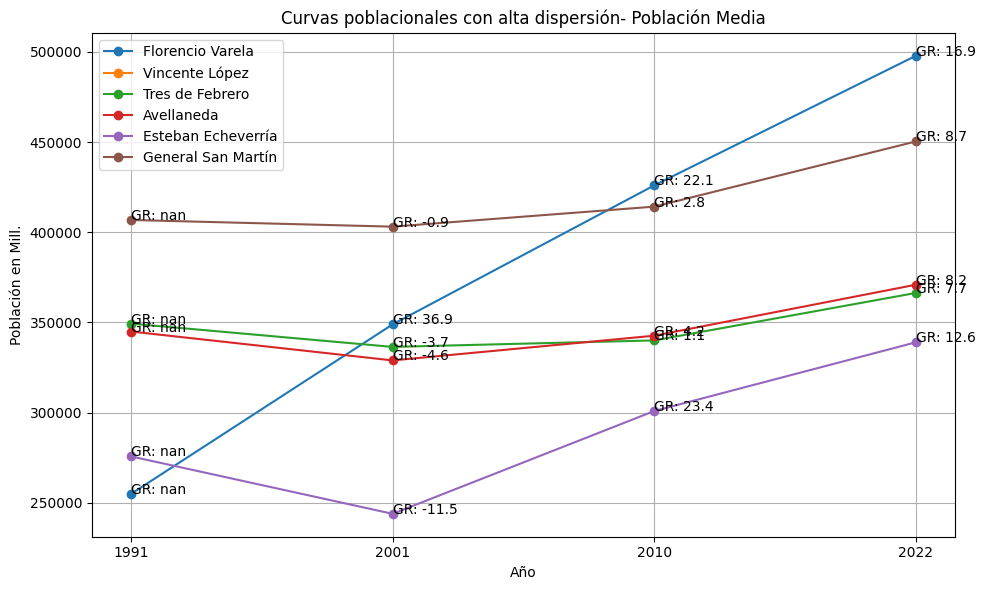
\includegraphics[width=0.8\textwidth]{{C:/Users/Fer/ITBA_TFI/code/latex/img/CurvasCVOutliersPobMedia.png}}
  \caption{Curvas poblacionales de alta dispersión - Población Media}
  \label{fig:CVoutCurvasMedia}
\end{figure}

\begin{figure}[htbp]
  \centering
  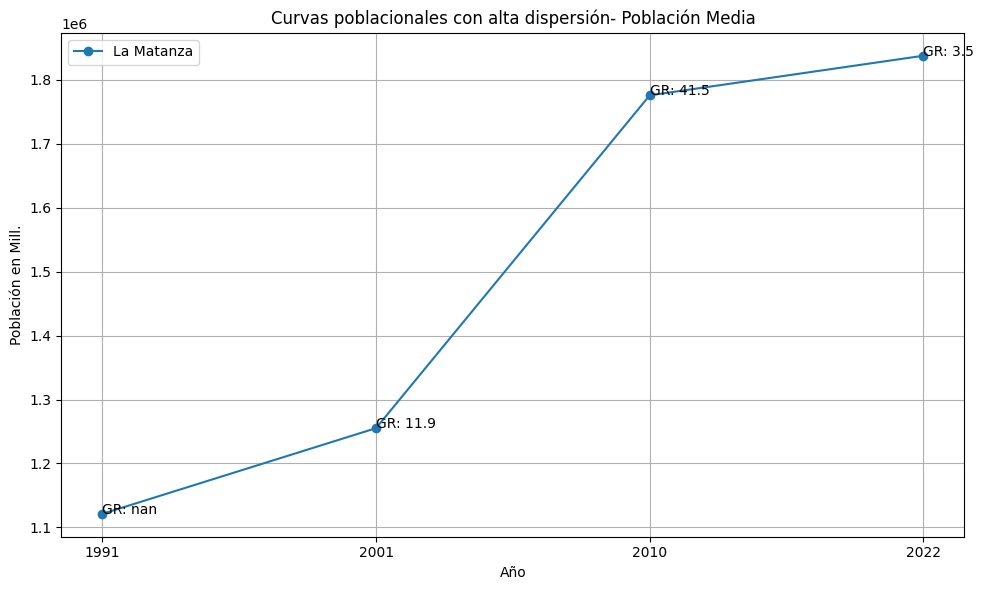
\includegraphics[width=0.8\textwidth]{{C:/Users/Fer/ITBA_TFI/code/latex/img/CurvasCVOutliersPobAlta.png}}
  \caption{Curvas poblacionales de alta dispersión - Población Alta}
\label{fig:CVoutCurvasAlta}
\end{figure}


\subsection{Densidad de Población}

En el dataset se incorpora la densidad de población en habitantes/\textup{km\textsuperscript{2}}. Si analizamos la distribución de los valores de
 densidad para cada censo, puede observarse distribuciones homogeneas simétricas, con un incremento en la mediana de cada población censal desde 2001 a 2022. 
 El análisis univariado de esta variable puede observarse en las Figuras \ref{fig:DensPoblBoxplot}  y \ref{fig:DensPoblLineas}.

\begin{figure}[htbp]
  \centering
  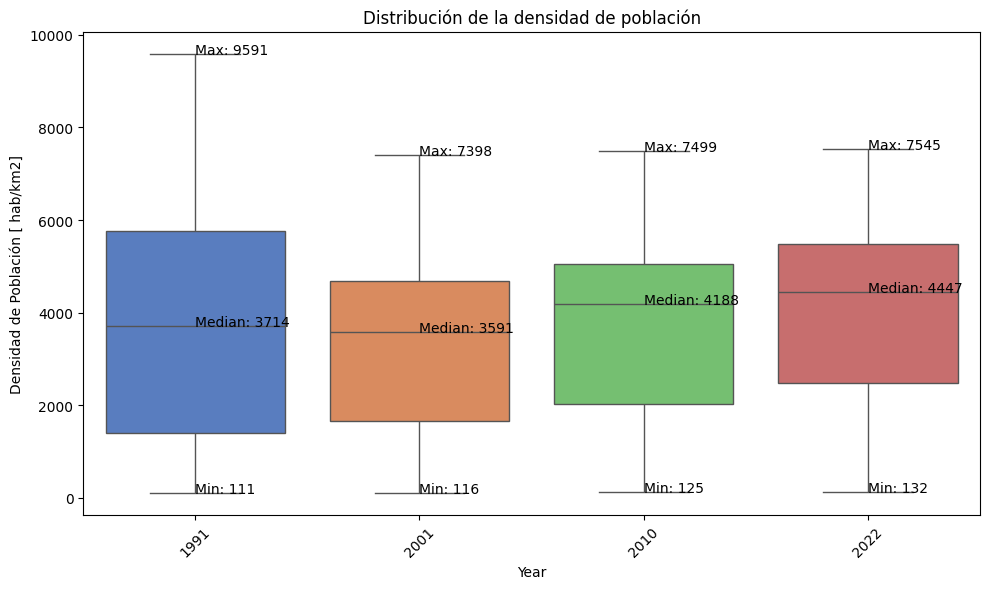
\includegraphics[width=0.8\textwidth]{{C:/Users/Fer/ITBA_TFI/code/latex/img/DensPobBoxplotxAnio.png}}
  \caption{Densidad de Población.Análisis Univariado}
  \label{fig:DensPoblBoxplot}
\end{figure}

\begin{figure}[htbp]
  \centering
  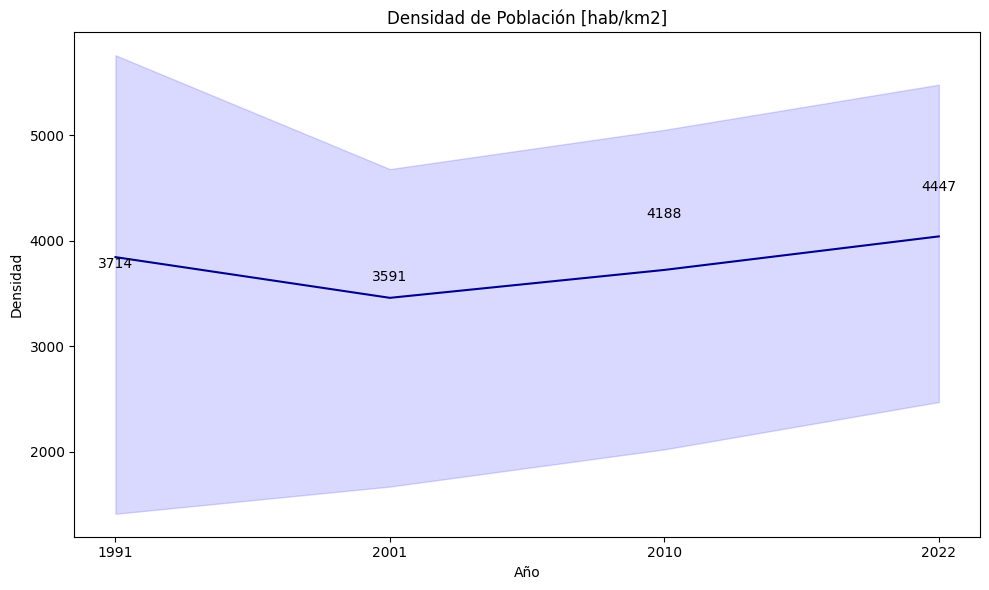
\includegraphics[width=0.8\textwidth]{{C:/Users/Fer/ITBA_TFI/code/latex/img/DensPobTendenciaLinea.png}}
  \caption{Densidad de Población.Análisis Univariado}
  \label{fig:DensPoblLineas}
\end{figure}


Se presenta también la distribución geográfica de la densidad por departamento para los censos analizados.
Si bien el distrito más poblado  es La Matanza, debido su extensión,  no es el departamento con mayor densidad poblacional 
en hab/\textup{km\textsuperscript{2}}. Como puede verse en la Figura \ref{fig:DensidadAll}, los distritos más densamente poblados son Lanús y Vicente López. 


\begin{landscape}
  \begin{figure}[p] % Use 'p' to force the figures to be placed on a separate page
    \centering
    \begin{subfigure}[b]{0.48\textwidth}
        \centering
        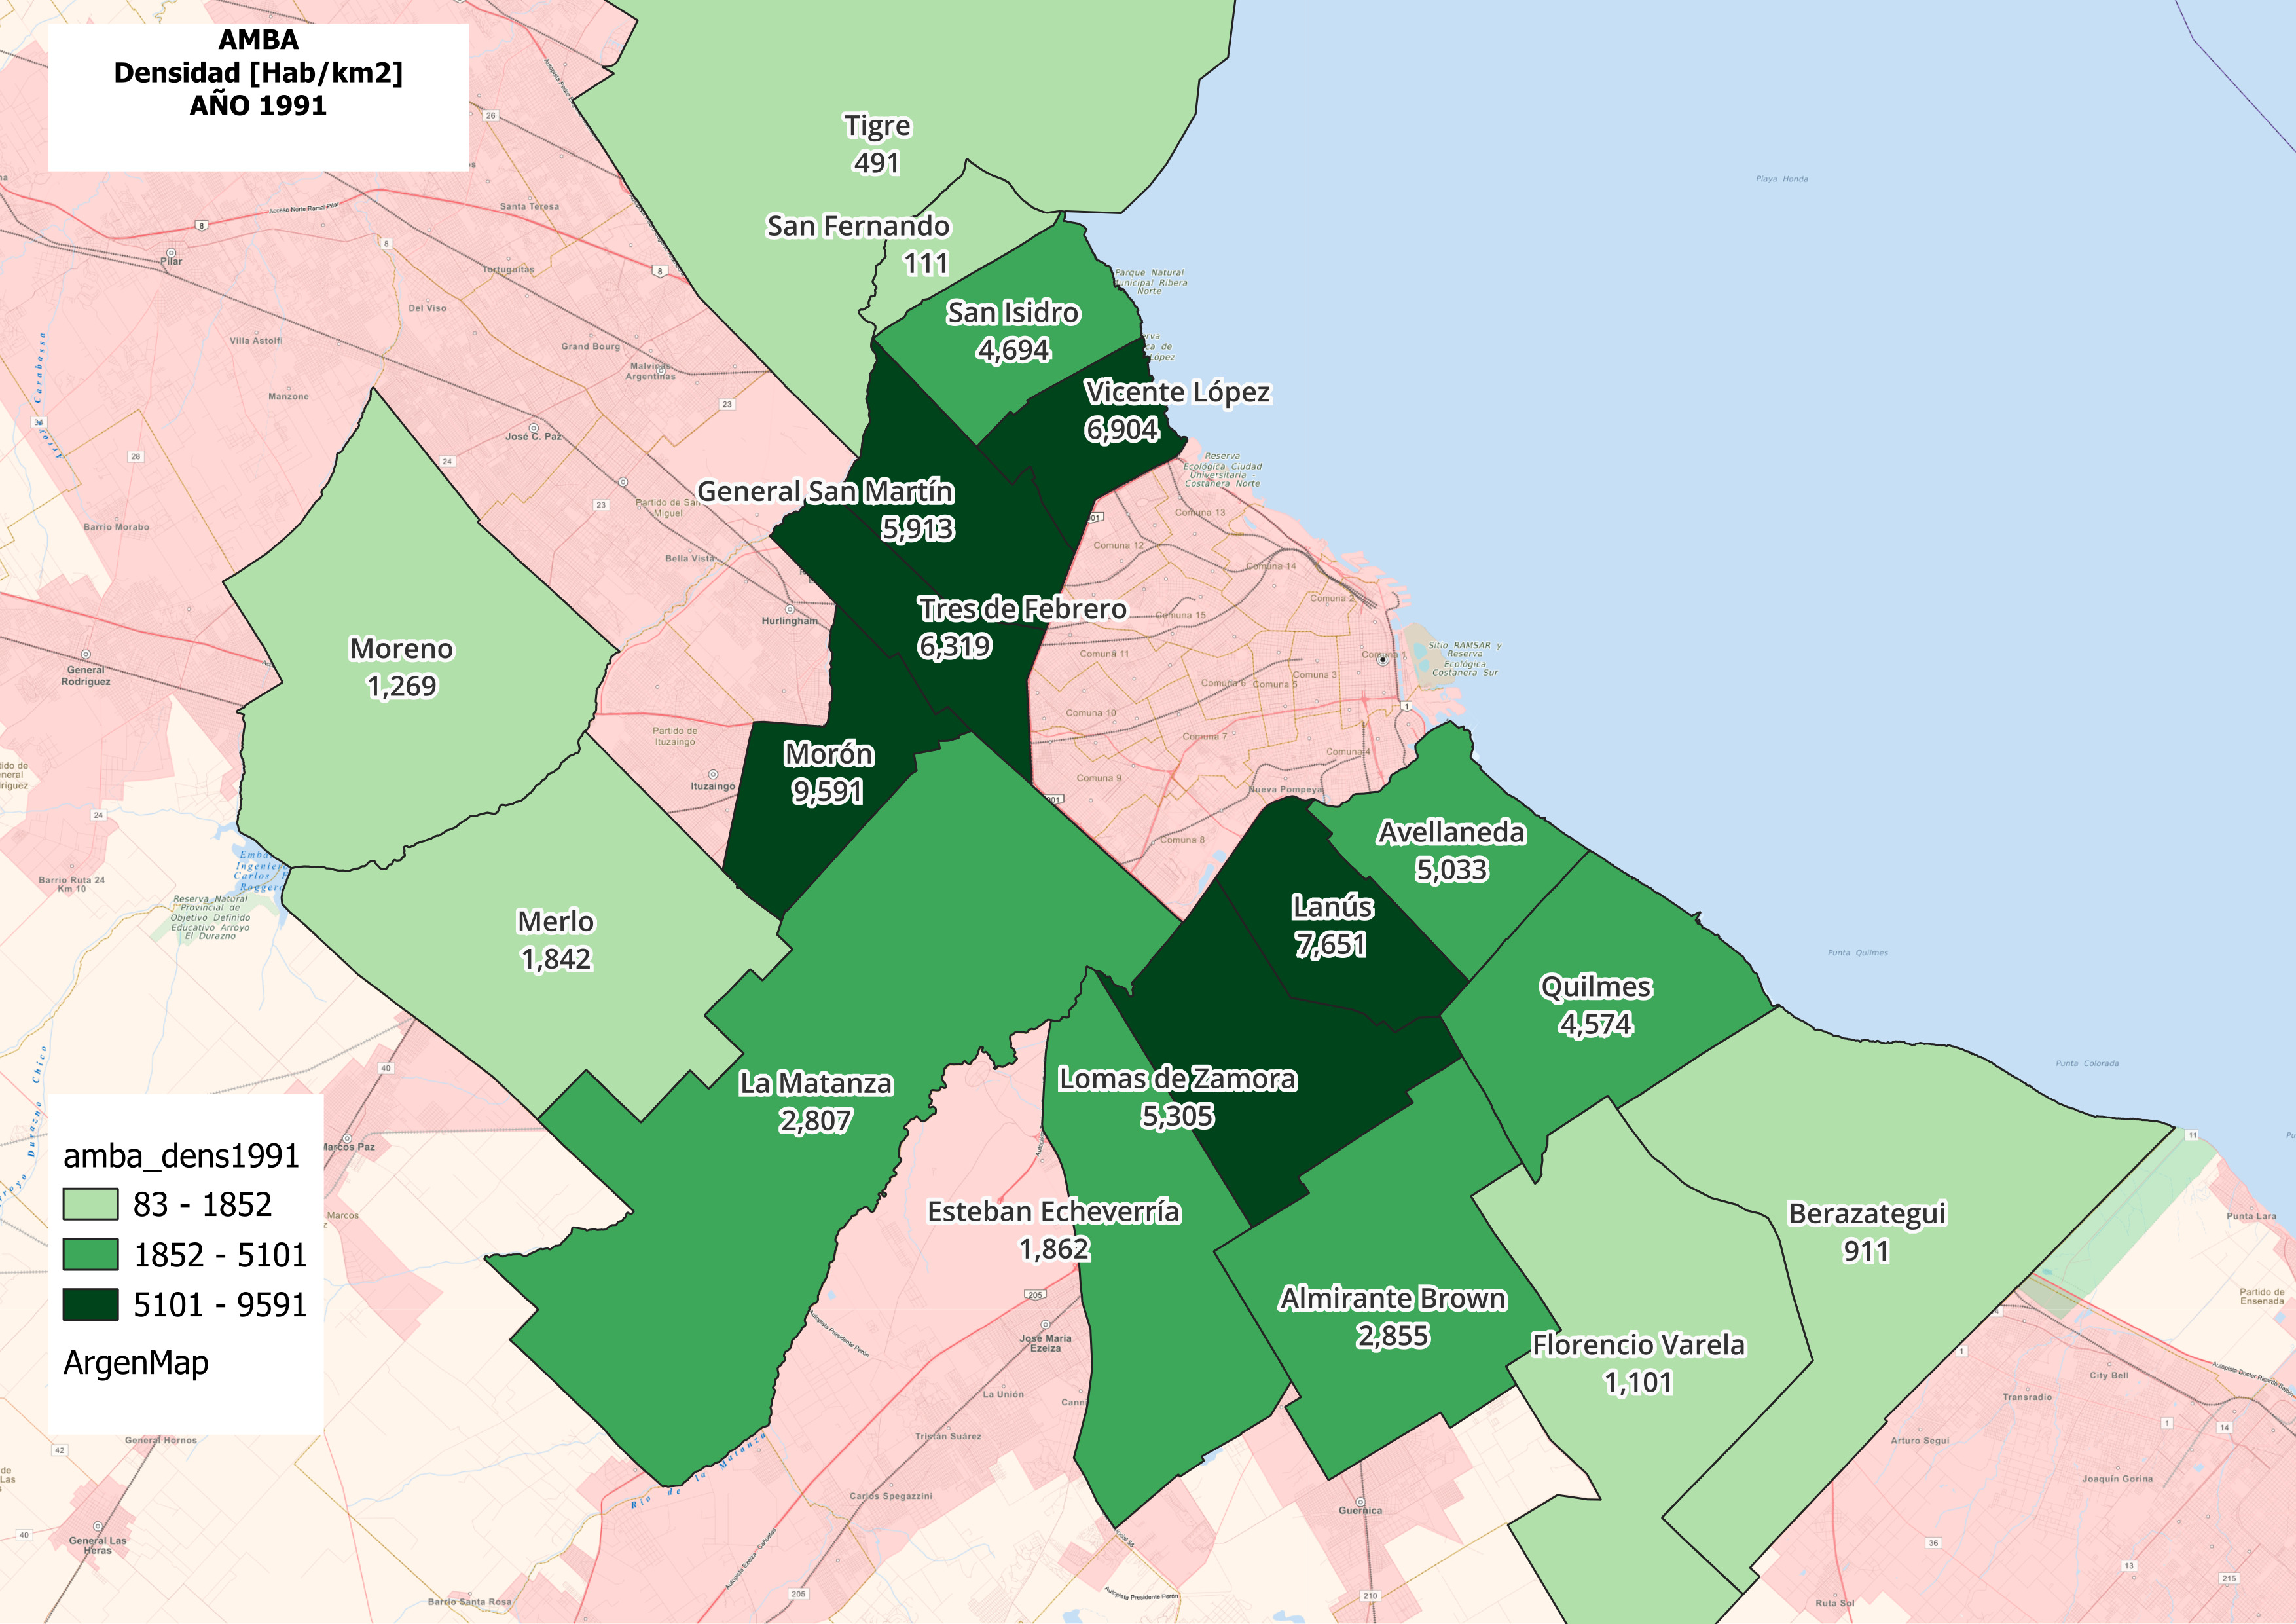
\includegraphics[width=\textwidth]{{C:/Users/Fer/ITBA_TFI/QGIS/img/AmbaDens1991.jpg}}
        \caption{AMBA- Población total Censo 1991}
    \label{fig:dens1991}
    \end{subfigure}
    \quad % Add some horizontal space between subfigures
    \begin{subfigure}[b]{0.48\textwidth}
        \centering
        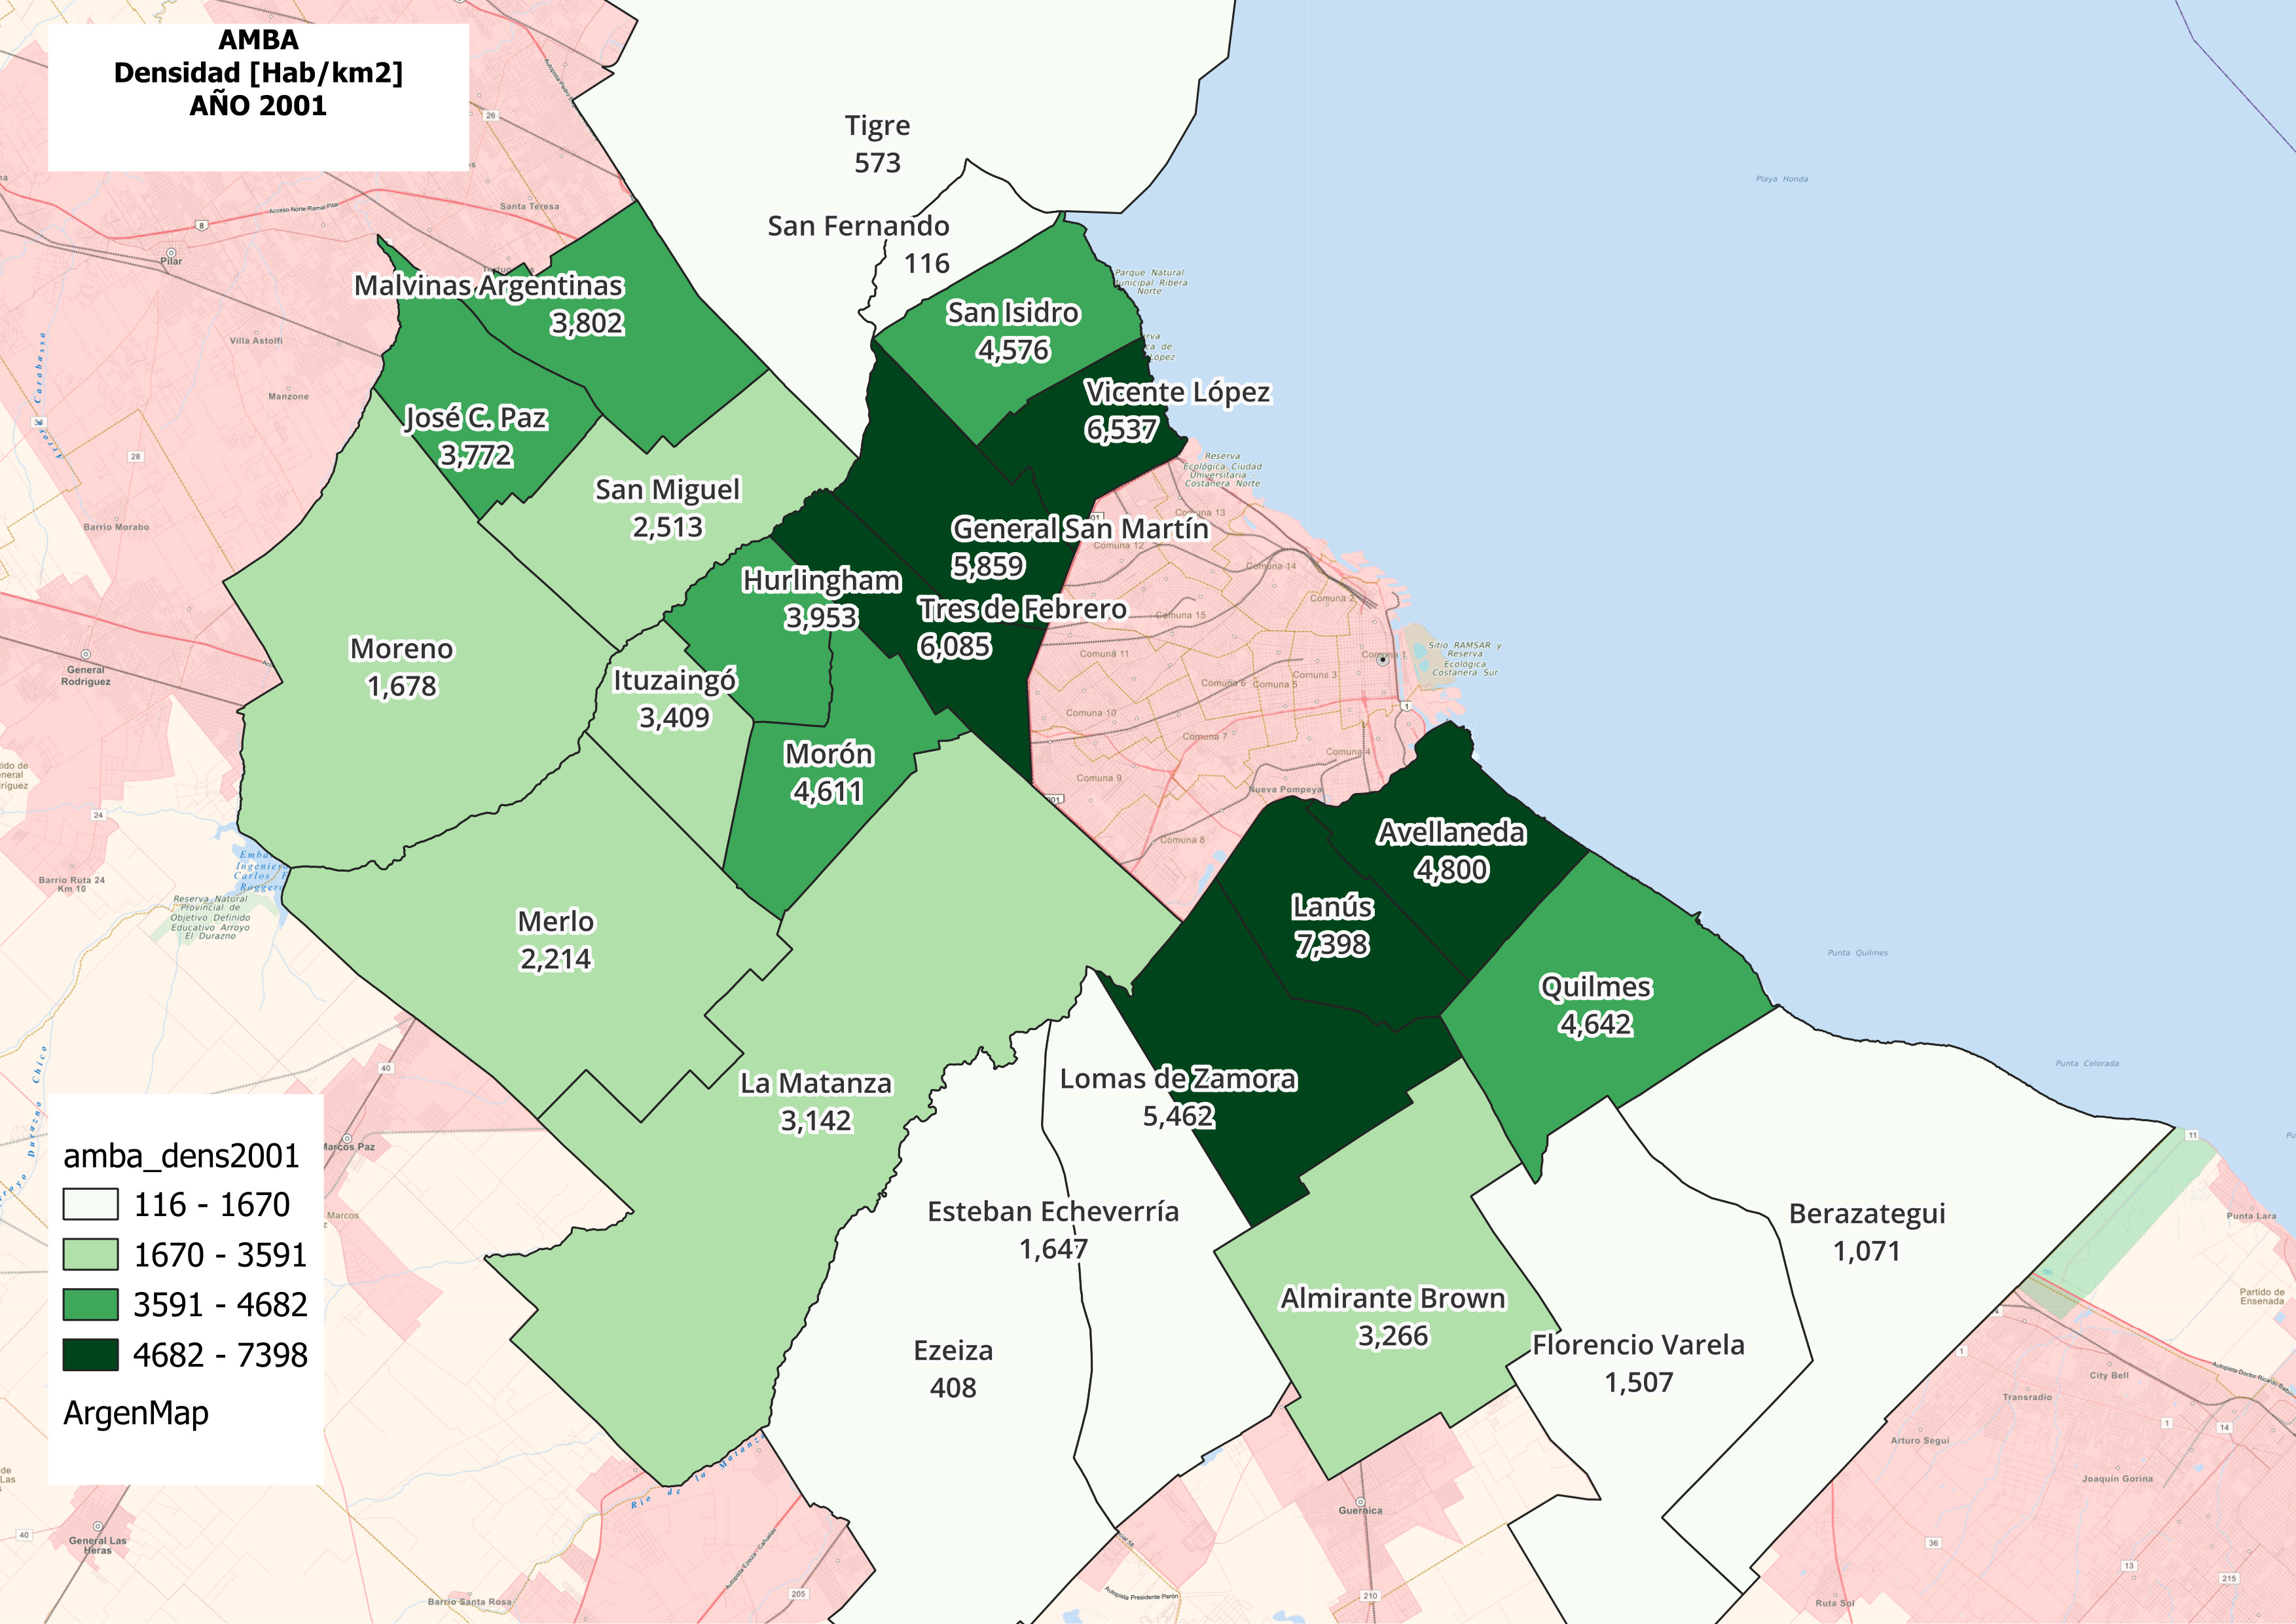
\includegraphics[width=\textwidth]{{C:/Users/Fer/ITBA_TFI/QGIS/img/AmbaDens2001.jpg}}
        \caption{AMBA- Densidad [hab/km2] Censo  2001}
      \label{fig:dens2001}
    \end{subfigure}
    \begin{subfigure}[b]{0.48\textwidth}
        \centering
        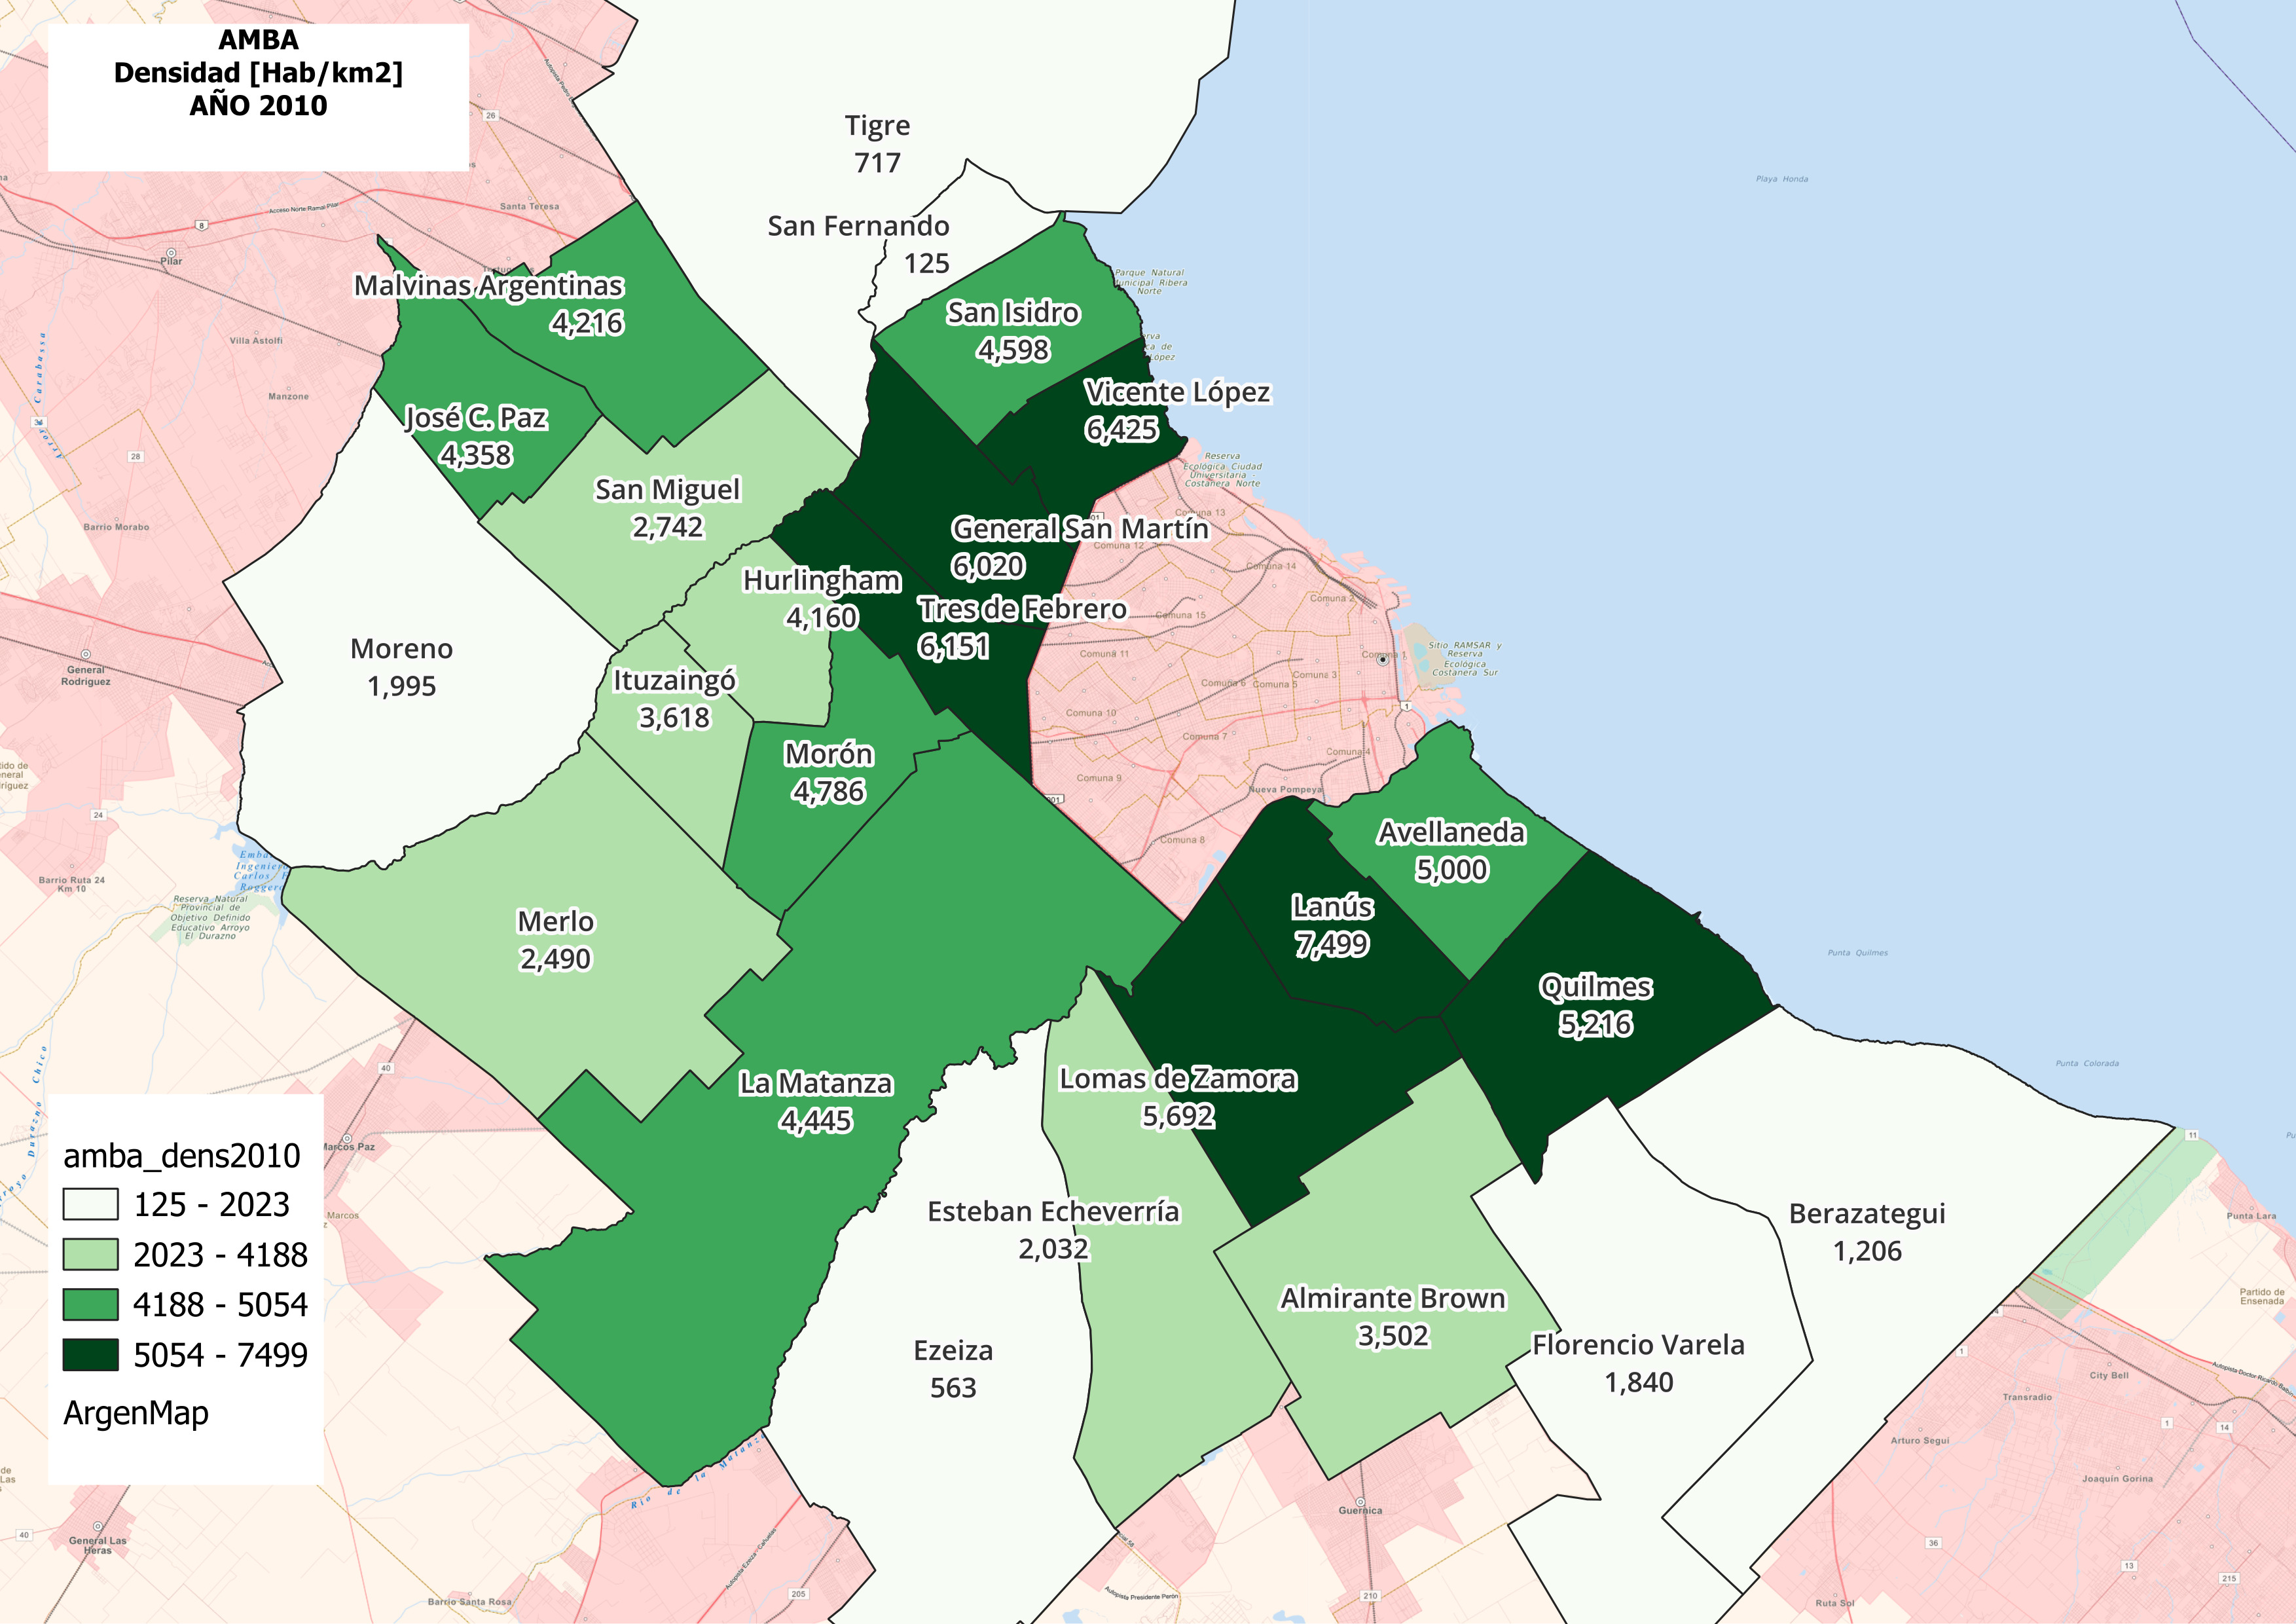
\includegraphics[width=\textwidth]{{C:/Users/Fer/ITBA_TFI/QGIS/img/AmbaDens2010.jpg}}
        \caption{AMBA- Densidad [hab/km2] Censo 2010}
      \label{fig:dens2010}
    \end{subfigure}
    \quad % Add some horizontal space between subfigures
    \begin{subfigure}[b]{0.48\textwidth}
        \centering
        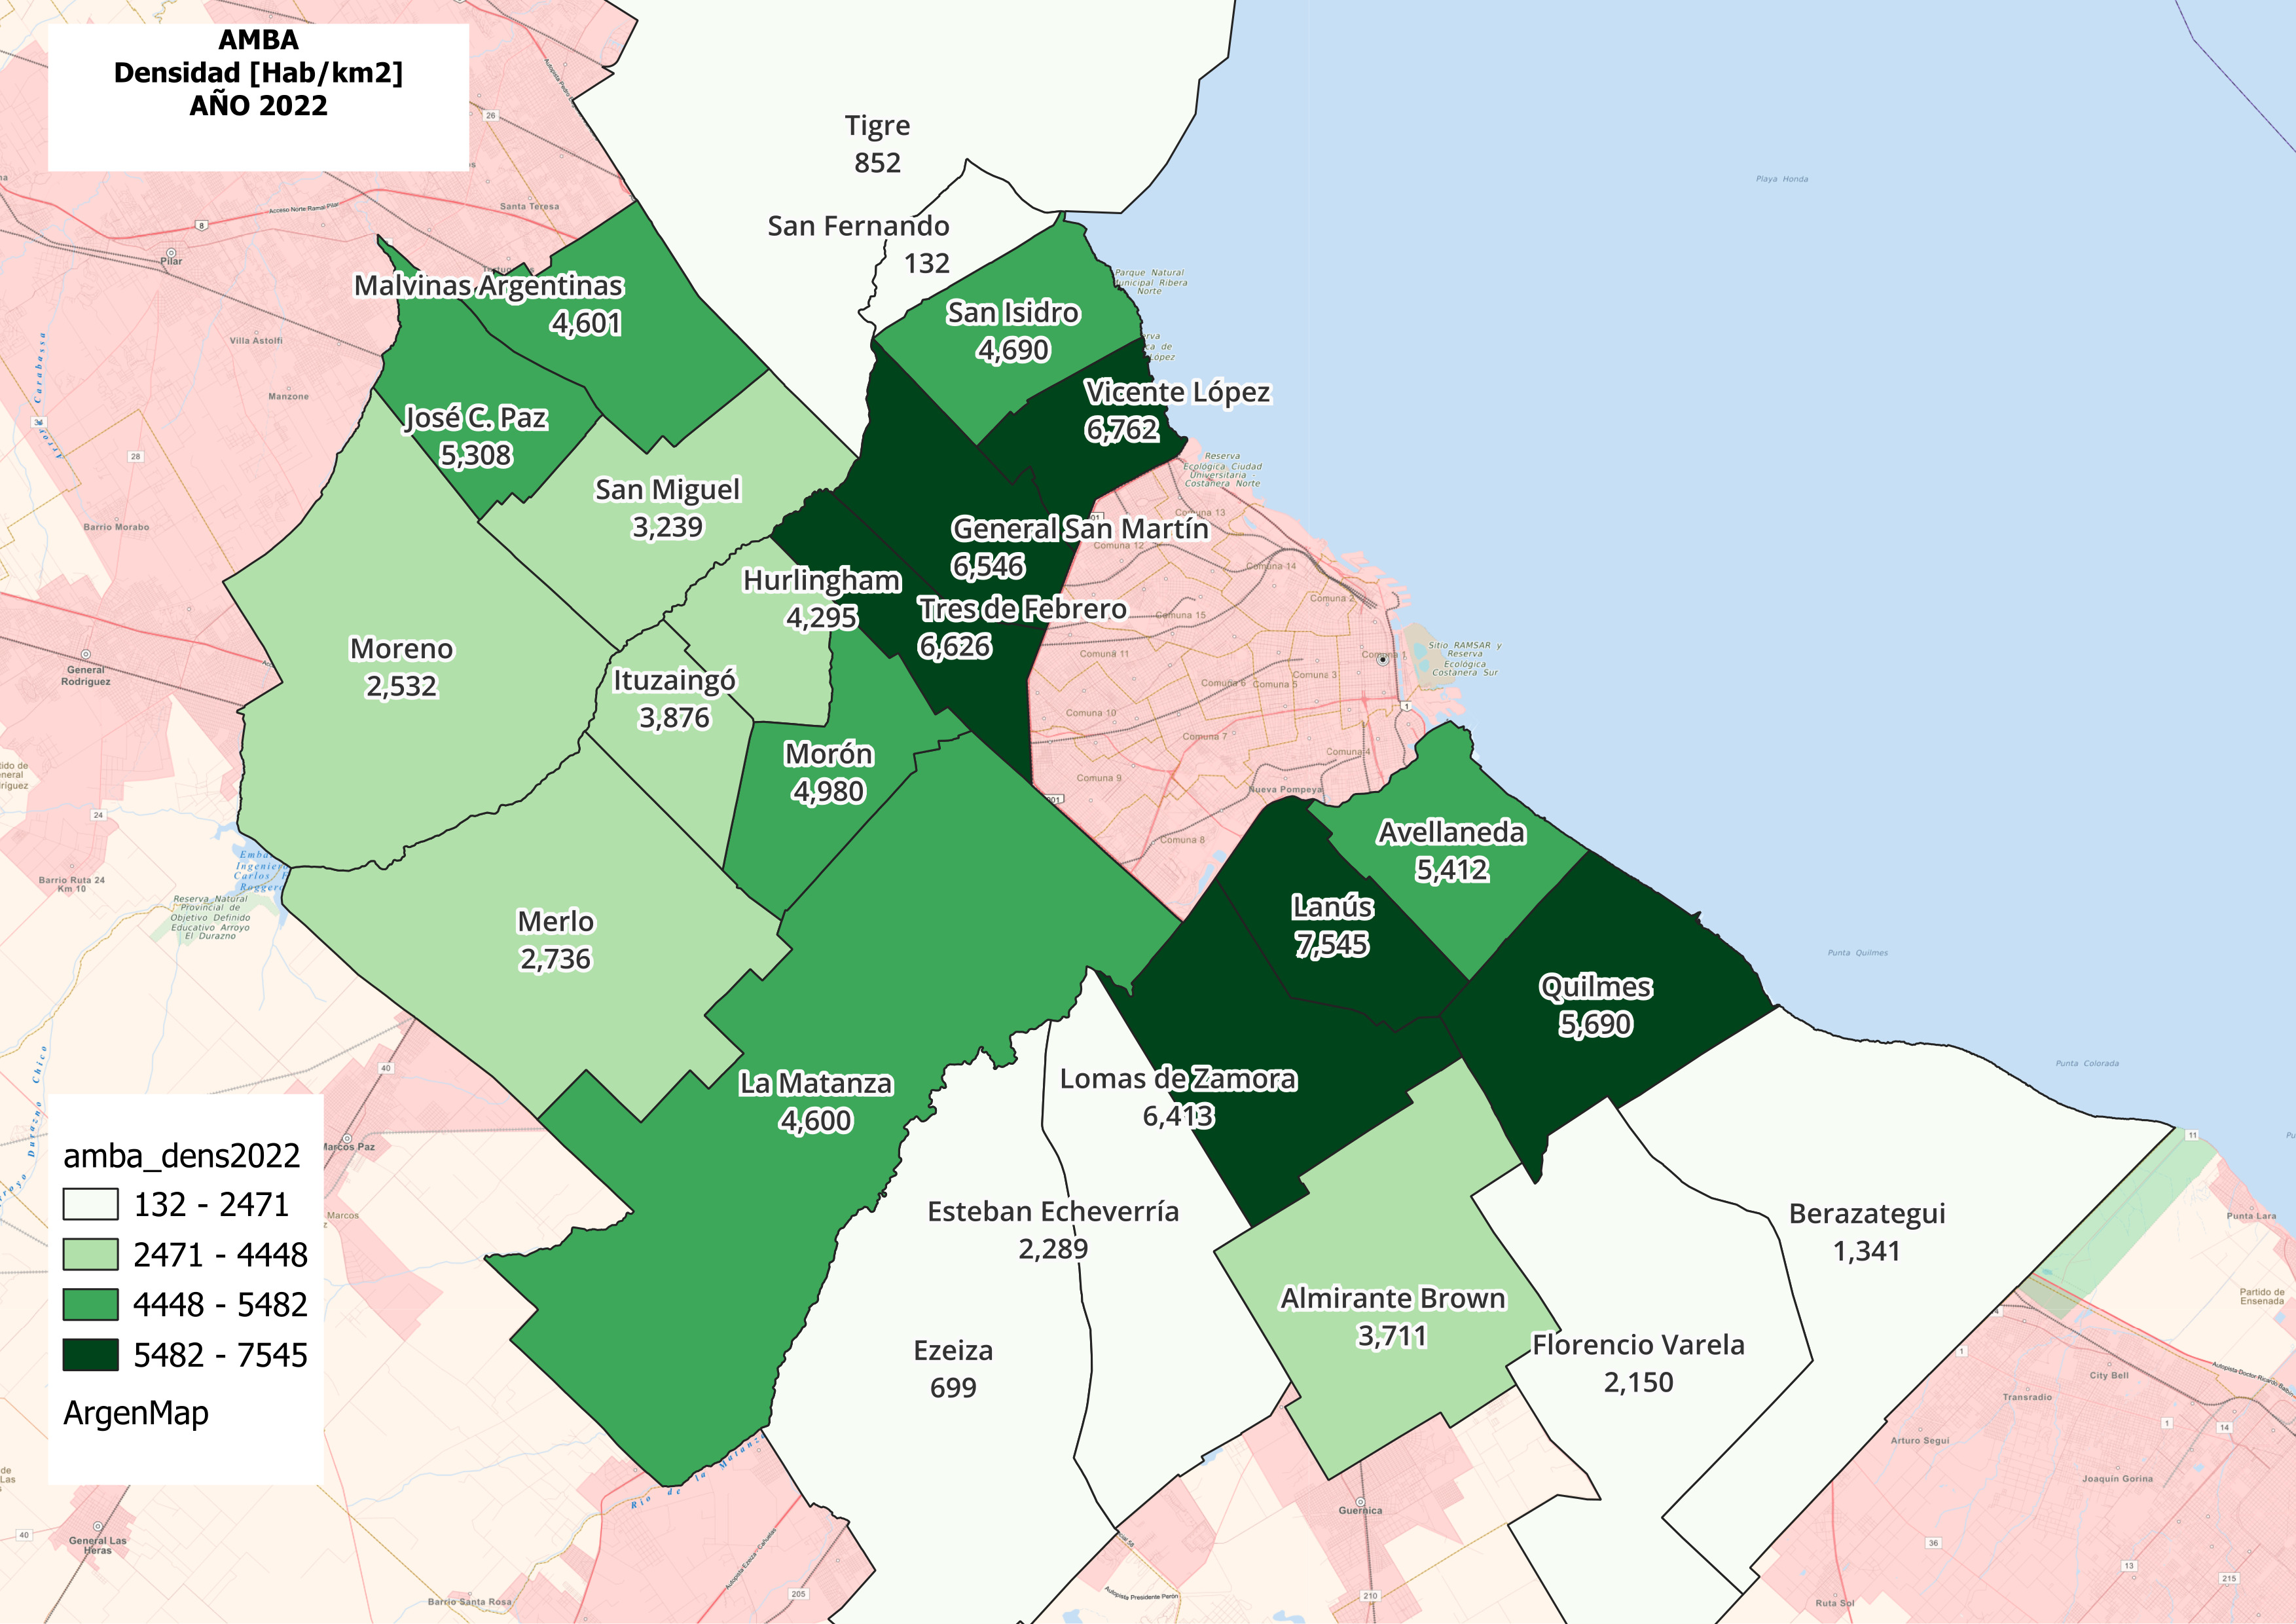
\includegraphics[width=\textwidth]{{C:/Users/Fer/ITBA_TFI/QGIS/img/AmbaDens2022.jpg}}
        \caption{AMBA- Densidad [hab/km2] Censo 2022}
      \label{fig:dens2022}
    \end{subfigure}
    \caption{AMBA- Densidad [hab/km2] Censos 1991 2022}
  \label{fig:DensidadAll}
  \end{figure}
  \end{landscape}
  

\subsection{Tipo de Vivienda}
A partir del censo 2001 se incorpora como atributo descriptivo en cada censo la composición  o tipo de la vivienda, ya sea de tipo particular o colectiva.
Se detalla en cada caso la cantidad de viviendas partculares ('vivpart') en determinado departamento, así como la cantidad de viviendas
colectivas presentes. Se presenta entonces la posibilidad de realizar un analisis univarido del porcentaje de viviendas particulares
respecto al total de viviendas para un determinado departamento y año censal. Para ello, se agrega al dataset una nueva variable definida como:
\begin{equation}
  {\text{VivPart\%}} = 
 \frac{\text{VivPart}}{\text{VivPart} +\text{VivColTot}} \times 100
\end{equation}
Surge de inmediato que la mayoría de la población vive en viviendas particulaes (mayor a 99.9\%). Al analizar el comportamiento de este indicador se 
observa un leve incremento sostenido en el tiempo desde 1991 hasta 2022. Es decir, se observan cada vez más peso de las viviendas particulares. 
El análisis univarido de este indicador puede observarse en las Figuras \ref{fig:VivpartBoxplot} y \ref{fig:VivpartLines}.


\begin{figure}[htbp]
  \centering
  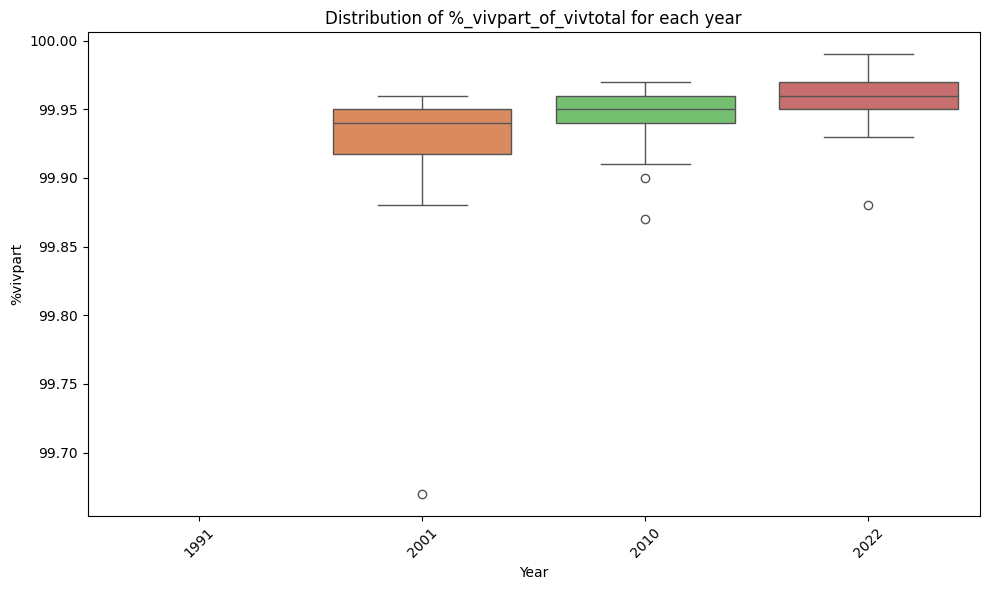
\includegraphics[width=0.8\textwidth]{{C:/Users/Fer/ITBA_TFI/code/latex/img/VivPartxanioBoxplot.png}}
  \caption{Composición de viviendas.Análisis Univariado}
  \label{fig:VivpartBoxplot}
\end{figure}

\begin{figure}[htbp]
  \centering
  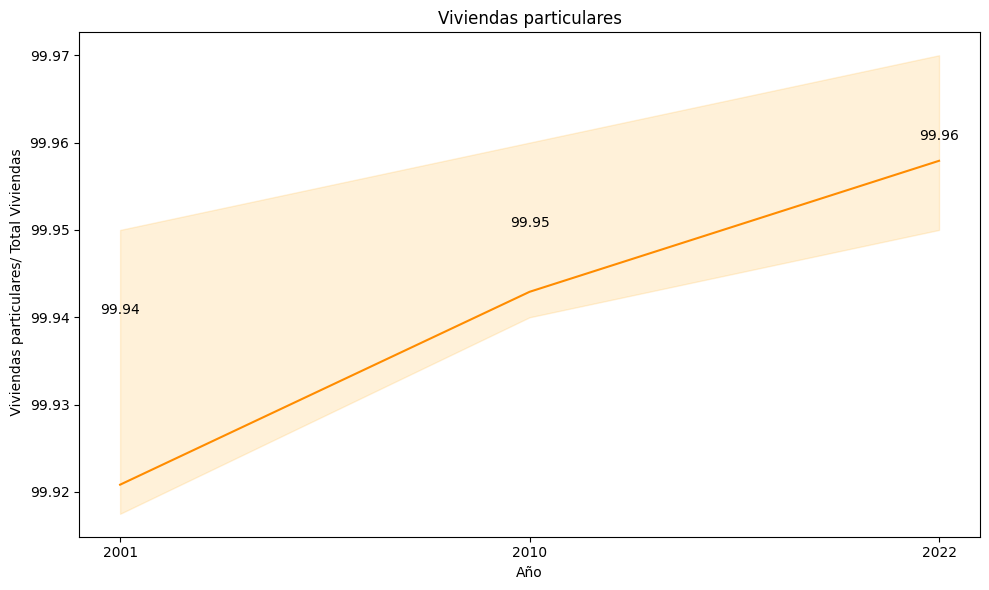
\includegraphics[width=0.8\textwidth]{{C:/Users/Fer/ITBA_TFI/code/latex/img/VivPartTendenciaLinea.png}}
  \caption{Composición de viviendas.Análisis Univariado}
  \label{fig:VivpartLines}
\end{figure}



\subsection{Índice de Masculinidad}
Un indicador habitual de las muestras poblacionales es el índice de masculinidad, que resultada de dividir el número de hombres entre el número de mujeres de una unidad geográfica o administrativa, 
expresado como porcentaje:

\begin{equation}
  {\text{IndMasc}} = 
 \frac{\text{Varones}}{\text{Mujeres}} \times 100
\end{equation}
Al analizar el comportamiento de este índice a lo largo del tiempo, se observa un descenso sostenido del mismo desde 1991 hasta 2022.
Particularmente el máximo de la muestra presenta un descenso de 5 puntos porcenturales para el año 2022, así como 2 puntos porcentuales en la mediana. Este resultado puede observarse 
en las Figuras \ref{fig:IndMascBox} y \ref{fig:IndMAsvLinea}.
\begin{figure}[htbp]
  \centering
  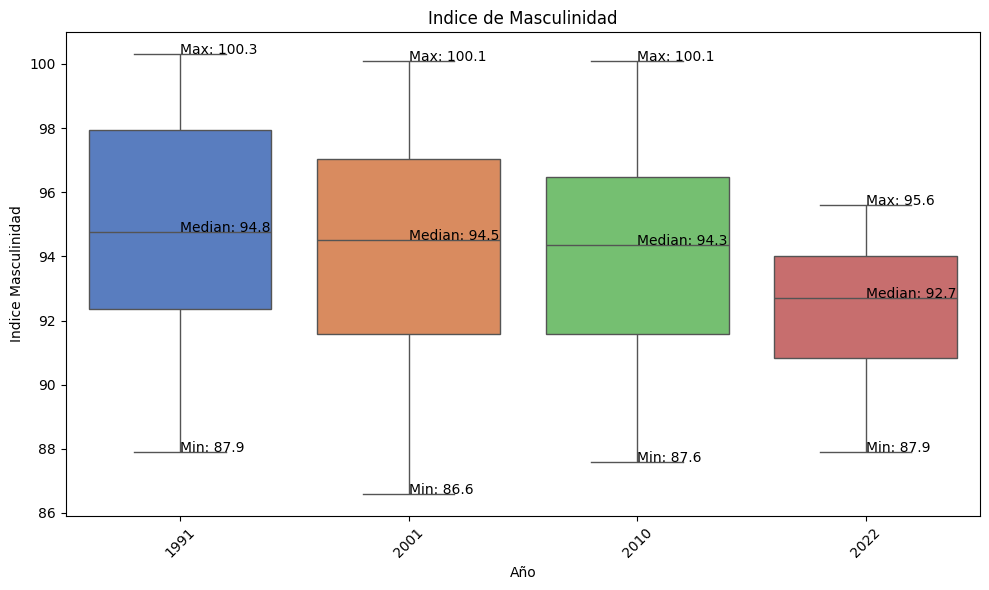
\includegraphics[width=0.8\textwidth]{{C:/Users/Fer/ITBA_TFI/code/latex/img/indMascxAnioBoxplot.png}}
  \caption{Índice de Masculinidad.Análisis Univariado}
\label{fig:IndMascBox}
\end{figure}

\begin{figure}[htbp]
  \centering
  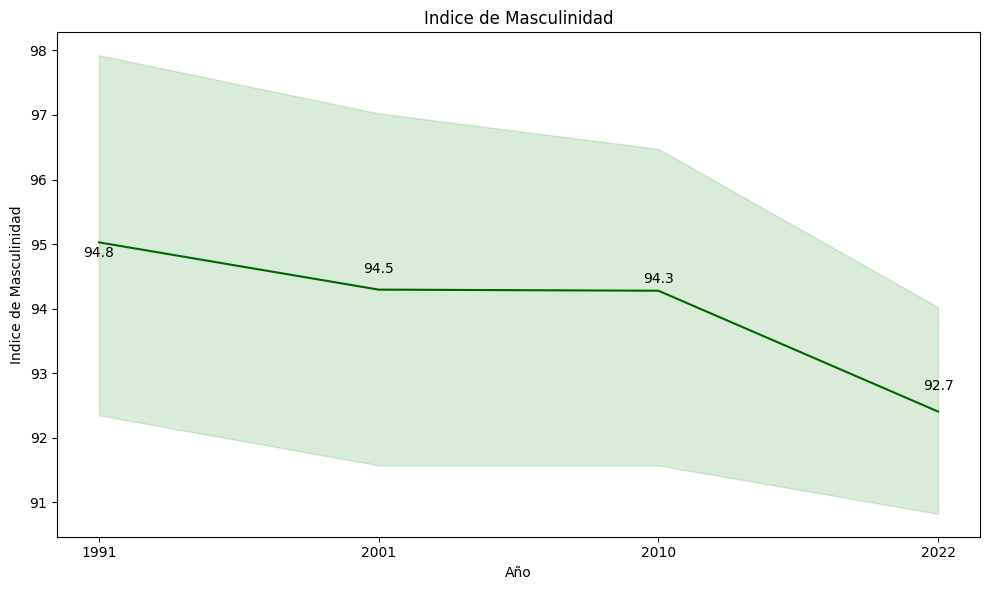
\includegraphics[width=0.8\textwidth]{{C:/Users/Fer/ITBA_TFI/code/latex/img/indMascTendenciaLinea.png}}
  \caption{Índice de Masculinidad.Análisis Univariado}
\label{fig:IndMAsvLinea}
\end{figure}

\section{ Compartiva de los Modelos de Predicción}
En base a los censos 1991,2001 y 2010, sumado a las variables sintomáticas antes descriptas, 
se pretende ajustar y entrenar los modelos para luego predecir la población total de cada departmento del AMBA para el Año 2022.
 Al comparar con los resultados publicados por INDEC para el censo 2022 \customcite{Censo2022Datos} se determinó la precisión de cada métodología aplicada.\newline
 Muchas de estas herramientas tiene problemas con los valores nulos o faltantes. Es por esto que los departamentos que no existían en 1991, demandaron 
un tratamiento  especial.
\subsection{Variables Censales}
Respecto a las variables censales podemos decir que presentan una correlación lineal directa muy imporante y
no aportan variabilidad. Por este motivo no son atributos sginificativos para los modelos propuestos. 
Para su análisis se utlizó la matriz de correlación, que puede verse en la Figura \ref{fig:MatCorr}. \newline
 \begin{figure}[htbp]
  \centering
  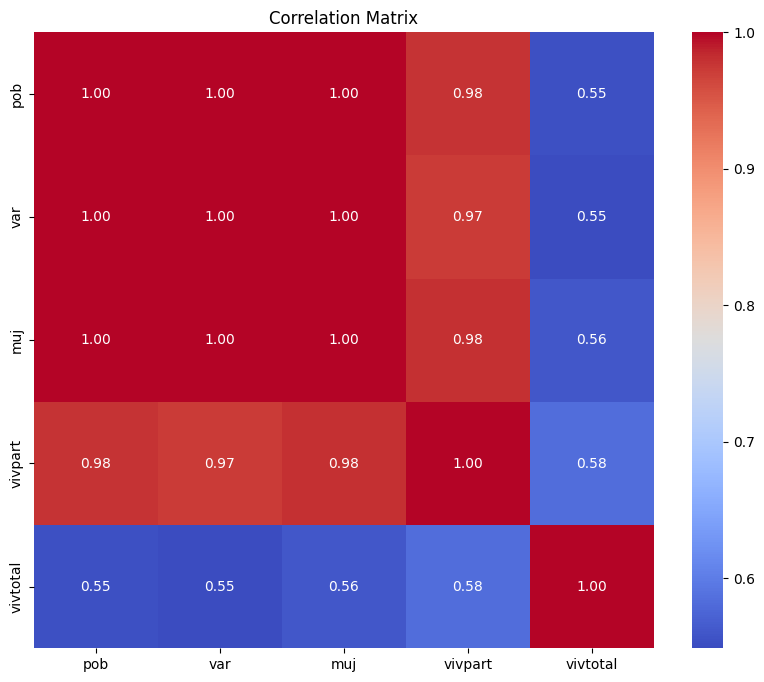
\includegraphics[width=0.75\textwidth]{{C:/Users/Fer/ITBA_TFI/code/latex/img/CorrMatrx.png}}
  \caption{Matriz de correlación .Variables Censales}
  \label{fig:MatCorr}
\end{figure}

\subsection{Errores típicos}
Para determinar la precisión y realizar la comparativa entre los modelos aplicados se recurrió a los errores típicos: Error Cuadrático Medio (Mean Squared Error, MSE), 
Raíz del Error Cuadrático Medio (Root Mean Squared Error, RMSE) y Error Porcentual Absoluto Medio (Mean Absolute Percentage Error, MAPE).\newline

MSE es una medida de la calidad de un estimador. Se calcula promediando el cuadrado de los errores (diferencias entre los valores predichos y los valores reales):

  \[
    \text{MSE} = \frac{1}{n} \sum_{i=1}^{n} (y_i - \hat{y}_i)^2
  \]

  RMSE es la raíz cuadrada del MSE, y proporciona una medida de la magnitud promedio del error en las mismas unidades que los valores predichos:
\[
\text{RMSE} = \sqrt{\frac{1}{n} \sum_{i=1}^{n} (y_i - \hat{y}_i)^2}
\]
 
MAPE es una medida de precisión que expresa el error como un porcentaje, y se calcula promediando el valor absoluto de los errores porcentuales:
\[
\text{MAPE} = \frac{100\%}{n} \sum_{i=1}^{n} \left| \frac{y_i - \hat{y}_i}{y_i} \right|
\]

\subsection{Dataset para Entrenamiento}

Como se mencionó en las secciones anteriores, se trabajó con los censos de los años 1991 , 2001 y 2010, conjunto al que se le agregó el valor
 de las variables sintomáticas para la Jurisdicción provincial- Provincia de Buenos Aires para dichos años.
Se tomó el enfoque planteado por \customcite{CELADEAlvarez}, entendiendo que el comportamiento de estas variables puede ayudar a explicar fenómenos a nivel departamental.
 Un fragmento del dataset utlizado como input de los modelos puede verse en el Cuadro \ref{tab:baseModelos}.


 % Place the table on a landscape page
\afterpage{
    \begin{landscape} 
     \begin{table}[htb]
     \centering
      \footnotesize
      \begin{tabular}{|c|c|c|c|c|c|c|c|c|c|c|c|c|c|c|c|c|}
        \hline
        \textbf{\cellcolor[rgb]{0,0.231,0.427}\textcolor{white}{Departamento}} & \textbf{\cellcolor[rgb]{0,0.231,0.427}\textcolor{white}{$cod_depto$}} & \textbf{\cellcolor[rgb]{0,0.231,0.427}\textcolor{white}{ano}} & \textbf{\cellcolor[rgb]{0,0.231,0.427}\textcolor{white}{pob}} & \textbf{\cellcolor[rgb]{0,0.231,0.427}\textcolor{white}{var}} & \textbf{\cellcolor[rgb]{0,0.231,0.427}\textcolor{white}{muj}} & \textbf{\cellcolor[rgb]{0,0.231,0.427}\textcolor{white}{vivpart}} & \textbf{\cellcolor[rgb]{0,0.231,0.427}\textcolor{white}{vivtotal}} & \textbf{\cellcolor[rgb]{0,0.231,0.427}\textcolor{white}{sup}} & \textbf{\cellcolor[rgb]{0,0.231,0.427}\textcolor{white}{$ind_masc$}} & \textbf{\cellcolor[rgb]{0,0.231,0.427}\textcolor{white}{$dens_pob$}} & \textbf{\cellcolor[rgb]{0,0.231,0.427}\textcolor{white}{TMI}} & \textbf{\cellcolor[rgb]{0,0.231,0.427}\textcolor{white}{TGF}} & \textbf{\cellcolor[rgb]{0,0.231,0.427}\textcolor{white}{TBN}} & \textbf{\cellcolor[rgb]{0,0.231,0.427}\textcolor{white}{TBM}} & \textbf{\cellcolor[rgb]{0,0.231,0.427}\textcolor{white}{TCV}} & \textbf{\cellcolor[rgb]{0,0.231,0.427}\textcolor{white}{Mat1ria}} \\ \hline
        Almirante Brown & 6028 & 1991 & 450698.0 & 222042.0 & 228656.0 & nan & nan & 157.87 & 97.1 & 2854.87 & 24.2 & 2.6 & 18.4 & 7.9 & 10.5 & 1752994.0 \\
        Almirante Brown & 6028 & 2001 & 515556.0 & 252454.0 & 263102.0 & 143543.0 & 88.0 & 157.87 & 96.0 & 3265.7 & 15.0 & 2.3 & 16.9 & 8.2 & 8.7 & 1658221.0 \\
        Almirante Brown & 6028 & 2010 & 552902.0 & 270247.0 & 282655.0 & 156218.0 & 78.0 & 157.87 & 95.6 & 3502.26 & 12.0 & 2.5 & 18.9 & 8.4 & 10.5 & 1667278.0 \\
        Avellaneda & 6035 & 1991 & 344991.0 & 164243.0 & 180748.0 & nan & nan & 68.54 & 90.9 & 5033.43 & 24.2 & 2.6 & 18.4 & 7.9 & 10.5 & 1752994.0 \\
        Avellaneda & 6035 & 2001 & 328980.0 & 155450.0 & 173530.0 & 117200.0 & 59.0 & 68.54 & 89.6 & 4799.82 & 15.0 & 2.3 & 16.9 & 8.2 & 8.7 & 1658221.0 \\
        Avellaneda & 6035 & 2010 & 342677.0 & 162264.0 & 180413.0 & 121307.0 & 68.0 & 68.54 & 89.9 & 4999.66 & 12.0 & 2.5 & 18.9 & 8.4 & 10.5 & 1667278.0 \\
        Berazategui & 6091 & 1991 & 244929.0 & 120870.0 & 124059.0 & nan & nan & 268.91 & 97.4 & 910.82 & 24.2 & 2.6 & 18.4 & 7.9 & 10.5 & 1752994.0 \\
        Berazategui & 6091 & 2001 & 287913.0 & 141163.0 & 146750.0 & 81511.0 & 38.0 & 268.91 & 96.2 & 1070.67 & 15.0 & 2.3 & 16.9 & 8.2 & 8.7 & 1658221.0 \\
        Berazategui & 6091 & 2010 & 324244.0 & 158608.0 & 165636.0 & 96029.0 & 37.0 & 268.91 & 95.8 & 1205.77 & 12.0 & 2.5 & 18.9 & 8.4 & 10.5 & 1667278.0 \\
        Esteban Echeverría & 6260 & 1991 & 275793.0 & 136784.0 & 139009.0 & nan & nan & 148.12 & 98.4 & 1861.96 & 24.2 & 2.6 & 18.4 & 7.9 & 10.5 & 1752994.0 \\
        Esteban Echeverría & 6260 & 2001 & 243974.0 & 120110.0 & 123864.0 & 70535.0 & 26.0 & 148.12 & 97.0 & 1647.14 & 15.0 & 2.3 & 16.9 & 8.2 & 8.7 & 1658221.0 \\
        Esteban Echeverría & 6260 & 2010 & 300959.0 & 147980.0 & 152979.0 & 88164.0 & 26.0 & 148.12 & 96.7 & 2031.86 & 12.0 & 2.5 & 18.9 & 8.4 & 10.5 & 1667278.0 \\
        \hline
      \end{tabular}
      \caption{Subset de datos input.Primeras 15 filas. Censos 1991, 2001, 2010 enriquecidos con las variables sintomáticas}
    \label{tab:baseModelos}
    \end{table}
    \end{landscape}
 }

 \subsection{Predicciones Población año 2022}

 En base al dataset de datos predefinido, se entrenaron los distintos modelos para luego predecir el valor de población total en cada
 departamento para el año 2022. Las predicciones realizadas corresponden a  Regresión Lineal, CART, Random Forest , LightGMB, junto a las 
estimaciones realizadas por el INDEC en el año 2010 \customcite{INDECProyecciones1025}. Para cada estimación se obtuvieron los errores 
 típicos mencionados (MSE, RMSE, MAPE). En la sección \ref{ResultadosMetodlogias} del presente trabajo se presentan 
 los resutados para cada metodología a nivel de departamento.
 A modo de resumen en el siguiente cuadro \ref{tab:PredAndMape} se puede observar el valor del censo 2022,
  las proyecciones de cada metodología y el error medio absoluto porcentual (MAPE) por departamento.\newline

%% TABLE RESULTADOS AND MAPE
 \begin{table}[htb]
  \centering
  \footnotesize
  \begin{tabular}{|c|c|c|c|c|c|c|}
  \hline
  \textbf{\cellcolor[rgb]{0,0.231,0.427}\textcolor{white}{Departamento}} & \textbf{\cellcolor[rgb]{0,0.231,0.427}\textcolor{white}{Censo2022}} & \textbf{\cellcolor[rgb]{0,0.231,0.427}\textcolor{white}{PredLR}} & \textbf{\cellcolor[rgb]{0,0.231,0.427}\textcolor{white}{PredRT}} & \textbf{\cellcolor[rgb]{0,0.231,0.427}\textcolor{white}{PredRF}} & \textbf{\cellcolor[rgb]{0,0.231,0.427}\textcolor{white}{PredLGB}} & \textbf{\cellcolor[rgb]{0,0.231,0.427}\textcolor{white}{PredINDEC}} \\ \hline
  Almirante Brown & 585,852 & 602,696 (2.9\%) & 552,902 (5.6\%) & 521,336 (11.0\%) & 506,385 (13.6\%) & 605,271 (3.3\%) \\
  Avellaneda & 370,939 & 360,939 (2.7\%) & 342,677 (7.6\%) & 337,916 (8.9\%) & 338,883 (8.6\%) & 358,512 (3.4\%) \\
  Berazategui & 360,582 & 372,685 (3.4\%) & 287,913 (20.2\%) & 295,665 (18.0\%) & 285,695 (20.8\%) & 372,889 (3.4\%) \\
  Esteban Echeverría & 339,030 & 376,939 (11.2\%) & 243,974 (28.0\%) & 278,778 (17.8\%) & 273,575 (19.3\%) & 383,538 (13.1\%) \\
  Ezeiza & 203,283 & 223,608 (10.0\%) & 118,807 (41.6\%) & nan & nan & 229,276 (12.8\%) \\
  Florencio Varela & 497,818 & 528,718 (6.2\%) & 426,005 (14.4\%) & 367,660 (26.1\%) & 343,324 (31.0\%) & 533,446 (7.2\%) \\
  General San Martín & 450,335 & 428,981 (4.7\%) & 403,107 (10.5\%) & 409,244 (9.1\%) & 408,037 (9.4\%) & 426,556 (5.3\%) \\
  Hurlingham & 187,122 & 193,235 (3.3\%) & 181,241 (3.1\%) & nan & nan & 195,596 (4.5\%) \\
  Ituzaingó & 179,788 & 180,761 (0.5\%) & 167,824 (6.7\%) & nan & nan & 182,993 (1.8\%) \\
  José C. Paz & 323,918 & 313,678 (3.2\%) & 265,981 (17.9\%) & nan & nan & 314,878 (2.8\%) \\
  La Matanza & 1,837,774 & 2,469,853 (34.4\%) & 1,775,816 (3.4\%) & 1,437,887 (21.8\%) & 1,384,134 (24.7\%) & 2,374,149 (29.2\%) \\
  Lanús & 462,051 & 467,504 (1.2\%) & 453,082 (1.9\%) & 459,486 (0.6\%) & 460,302 (0.4\%) & 462,693 (0.1\%) \\
  Lomas de Zamora & 694,330 & 649,524 (6.5\%) & 591,345 (14.8\%) & 599,412 (13.7\%) & 593,985 (14.4\%) & 652,937 (6.0\%) \\
  Malvinas Argentinas & 351,788 & 364,620 (3.6\%) & 290,691 (17.4\%) & nan & nan & 366,479 (4.2\%) \\
  Merlo & 580,806 & 606,506 (4.4\%) & 528,494 (9.0\%) & 475,189 (18.2\%) & 463,112 (20.3\%) & 620,307 (6.8\%) \\
  Moreno & 574,374 & 548,507 (4.5\%) & 452,505 (21.2\%) & 389,610 (32.2\%) & 373,574 (35.0\%) & 558,068 (2.8\%) \\
  Morón & 334,178 & 336,747 (0.8\%) & 321,109 (3.9\%) & 381,258 (14.1\%) & 424,681 (27.1\%) & 317,584 (5.0\%) \\
  Quilmes & 636,026 & 668,483 (5.1\%) & 582,943 (8.3\%) & 544,713 (14.4\%) & 537,655 (15.5\%) & 679,375 (6.8\%) \\
  San Fernando & 172,524 & 179,385 (4.0\%) & 151,131 (12.4\%) & 155,854 (9.7\%) & 153,045 (11.3\%) & 176,795 (2.5\%) \\
  San Isidro & 298,777 & 294,708 (1.4\%) & 292,878 (2.0\%) & 293,647 (1.7\%) & 294,469 (1.4\%) & 291,704 (2.4\%) \\
  San Miguel & 326,215 & 306,995 (5.9\%) & 276,190 (15.3\%) & nan & nan & 308,784 (5.3\%) \\
  Tigre & 447,785 & 476,591 (6.4\%) & 301,223 (32.7\%) & 327,135 (26.9\%) & 311,842 (30.4\%) & nan \\
  Tres de Febrero & 366,377 & 344,876 (5.9\%) & 336,467 (8.2\%) & 341,817 (6.7\%) & 341,971 (6.7\%) & 344,172 (6.1\%) \\
  Vicente López & 283,510 & 263,204 (7.2\%) & 269,420 (5.0\%) & 277,881 (2.0\%) & 277,669 (2.1\%) & 266,880 (5.9\%) \\
  \hline
  \end{tabular}
  \caption{Predicciones de población según metodolgía (MAPE\%) por departamento.\newline
          LR : Regresión Lineal - RT: Árboles de Regresión (CART) - RF: Random Forest - LGB: LightGBM}
  \label{tab:PredAndMape}
  \end{table}
  
 
 Para la comparativa entre los modelos se evaluó el desempeño de cada modelo sobre los 24 departamentos del AMBA.
 En el cuadro \ref{tab:AvgErrors} se pueden observer el valor medio de los errores típicos para cada metodología,
  se considera el MAPE como principal indicador de desempeño. \newline 
 %% AVG ERRORS
 \begin{table}[htb!]
  \centering
  \begin{tabular}{|c|c|c|c|}
  \hline
  \textbf{\cellcolor[rgb]{0,0.231,0.427}\textcolor{white}{Method}} & \textbf{\cellcolor[rgb]{0,0.231,0.427}\textcolor{white}{MSE}} & \textbf{\cellcolor[rgb]{0,0.231,0.427}\textcolor{white}{RMSE}} & \textbf{\cellcolor[rgb]{0,0.231,0.427}\textcolor{white}{MAPE}} \\ \hline
  Linear Regression & 1.7e+10 & 43720.0 & 5.8 \\
  Regression Trees & 4.1e+09 & 52144.0 & 13.0 \\
  Random Forest & 1.5e+10 & 82930.0 & 14.0 \\
  LightGBM & 1.9e+10 & 94541.0 & 16.2 \\
  INDEC & 6.5e+09 & 80792.0 & 6.1 \\
  \hline
  \end{tabular}
  \caption{ Errores típicos por metodología. (Promedio)}
  \label{tab:AvgErrors}
\end{table}
  
 Los resultados obtenidos implican  que  las metodologías tradicionales aproximan mejor este tipo de datos poblacionales dispersos (''sparse''). Tanto la regresión Lineal ,
 como las proyecciones realizadas por el INDEC presentan mejor precisión- menor error- y una menor desviación estándar.
  Este comportamiento se puede
 observar  al  graficar el  Error Porcentual Absoluto Medio (MAPE) para cada metodolgía para las 24 proyecciones realizadas, figura \ref{fig:BoxPlotModelos}.\newline
  Las algoritmos de data mining presentan dificultades debido a las características particulares de la información censal, así como  el hecho de estar trabajando sólo con la información de 
 tres Censos Nacionales. Sumado a ésto, la granularidad analizada en este caso (nivel departamental) hace difícil enriquecer el dataset con variables sintomáticas a este nivel 
 y se debe recurrir a información agregada a nivel Provincial. Estos modelos presentan valores de error notablemente mayores y una amplia dispesión de resultados.\newline

\begin{figure}[htbp]
  \centering
  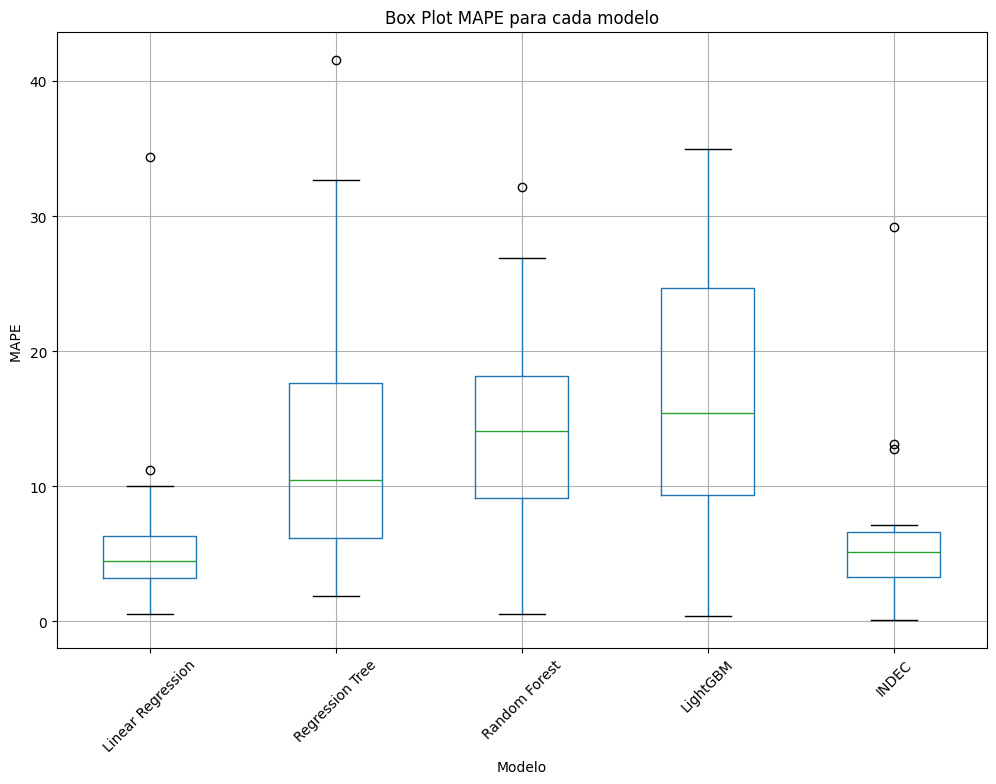
\includegraphics[width=0.8\textwidth]{{C:/Users/Fer/ITBA_TFI/code/latex/img/BoxPlotModels.png}}
  \caption{Box plot del Error Porcentual Absoluto Medio para cada modelo, sobre la predicción población año 2022. Todos los departamentos.}
  \label{fig:BoxPlotModelos}
\end{figure}

  

En cada modelo los outliers del boxplot son aquellos departamentos donde dicho modelo tuvo una muy mala performace relativa.
 Si se analizan los modelos con mejor precisión, en Regresión Lineal tanto
Esteban Echeverría (MAPE:11.2\%) como la Matanza (MAPE:41.6\%) son outliers, donde la predicción estuvo muy alejada del valor poblacional del censo 2022. 
Para el caso de las proyecciones según INDEC, aparecen también Esteban Echeverría (MAPE:13.1\%), Ezeiza (MAPE:12.8\%) y la Matanza (MAPE:29.2\%) como outiliers. 
 El caso de Esteban Echeverría tiene que ver con la cesión de territorio(cambio administrativo) desde el año 1991 al 2001. Esto implicó que su población descienda entre 1991  y 2001 un -11,5\% mientras que
 entre 2001 y 2010 creció un 23.3\%. Por ende Esteban Echeverría presenta una curva poblacional con un comportamiento particular, no producida 
 por el fenómeno demográfico. La Matanza no ha sufrido modificaciones territoriales en este periodo y por tanto presenta una curva
  poblacional con singularidades, con un comportamiento difenciado del resto de los departamentos.\newline


Al analizar la curva poblacional de La Matanza (ver Figura \ref{fig:LMFinalChart}), se observan cambios significativos en el
 ratio de crecimiento intercensal, a lo largo de los distintos censos.
Si se observa el año 2001 , el ratio intercensal es de 11.9\%, lo que se ubica un 75\% por encima del crecimento 
promedio (6.8\%) para los municipios del AMBA. En el año 2010 se observa un ratio de 41.5\%, que reprensenta un 250\% por 
encima del crecimiento promedio (11.8\%). Esto representa un salto importante, siendo el municipio con mayor crecimiento
en este periodo. Mientras que para el año 2022 se observa un ratio mucho menor, del orden de 3.5\%, un 70\% por debajo
 del crecimiento promedio (10.6\%).\newline

Esto implica que La Matanza es uno de los departamento con mayor desviación estandar y coeficiente de variación en
 tasas de crecimiento,  tal como se describió en apartados anteriores. El creciemiento promedio
  de los departamentos del AMBA para el periodo 1991 a 2010 es de 9,9\% , mientras que La Matanza en el mismo periodo
 creció un 26,7\% siendo uno de los municipios con mayor crecimiento poblacional.
 Obviamente el promedio cae al incorporar el año 2022, dando lugar a que La Matanza en toda la serie se acerque al
 crecimiento promedio de otros municipios.
Seguramente estas singulardidades hayan dificultado la predicción del valor poblacional para el deparamento con
 todas la metodologías aplicadas,  incluyendo aquellas que pudieron resultar más efectivas en la mayoría de los casos.

\begin{figure}[htbp]
  \centering
  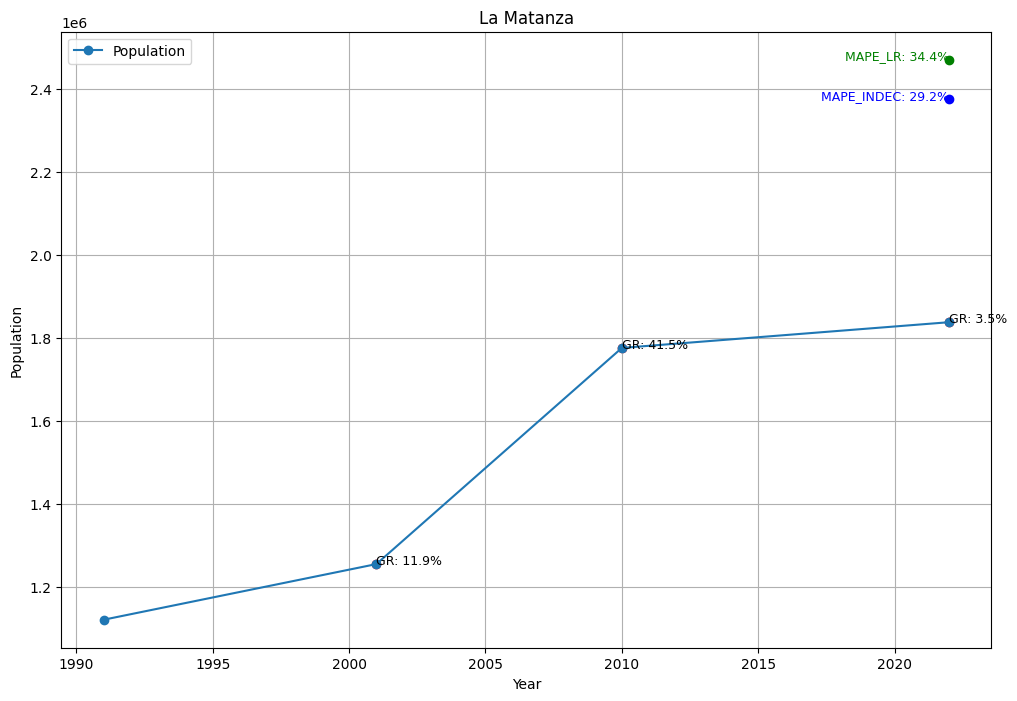
\includegraphics[width=0.8\textwidth]{{C:/Users/Fer/ITBA_TFI/code/latex/img/LMFinalChart.png}}
  \caption{Curva Poblacional La Matanza. GR:Ratio de crecmiento intercencsal.}
  \label{fig:LMFinalChart}
\end{figure} 

 
\section{Conclusiones y Trabajo Futuro} 

La información estadística que brindan las proyecciones de población representa un insumo vital en la planificación 
de políticas públicas de corto, mediano y largo plazo. Contar con esta información le permite al Estado determinar los recursos presupuestarios necesarios para satisfacer
la demanda potencial de bienes y servicios en distintas áreas. De hecho, en la provincia de Buenos Aires, ciertos aspectos del presupuesto son asignados en base a la población de cada municipio. 
Por este motivo, aunque en muchos casos dichas proyecciones se encuentran a nivel País o Provincia, es necesario contar con la información con un mayor nivel de desagregación (Municipios).\newline

La elaboración de proyecciones de población es una tarea compleja que debe ser realizada a través de un análisis exhaustivo que permita considerar los censos anteriores como también registros vitales y estimaciones de migración.
Aunque, en general, se ha utilizado el Método de las Componentes para elaborar dichas proyecciones, para el caso de las desagregación a nivel municipio, no resulta simple su aplcación, especialmente por la inestabilidad de la migración interna.
En Argentina, el Instituto Nacional de Estadísticas y Censos (INDEC) provee proyecciones de población a nivel nacional, desagregados a nivel departamental. Dichas estimaciones se apoyan en el crecimiento intercensal, que comprende la evolución en conjunto  de las tres variables básicas del análisis demográfico: la fecundidad, la mortalidad y la migración del período entre censos.\newline

El objetivo del presente trabajo consistió en demostrar que la tasa de crecimiento y curva poblacional en el período 1991-2022 de un municipio particular de la Provincia de Buenos Ares, la Matanza, presenta una singularidad en su curva de crecimiento poblacional, tanto en número de habitantes como en tasas intercensales, respecto a los municipios aledaños.\newline

Para llevar adelante este objetivo, se tomó la información censal del INDEC desde 1991 hasta 2022 para distintos niveles de granularidad, ya que en algunos casos no se presentan todas las variables. Sobre la misma, se realizó un trabajo de 
limpieza y pre-procesamiento importante, con enriquecimiento de datos geogáficos obtenidos desde el Instituto Geográfico Nacional. Para resolver el problema de los cambios de departamento en el tiempo, que ceden parte de su terreno o se fusionan, 
se utilizó el enfoque Slowly Changing Dimension Tipo 3, conservando en el registro el valor anterior, de qué otro departamento proviene y la superficie correspondiente asociada. Finalmente, sobre el dataset obtenido, se realizó un análisis 
exploratorio de cada variable., para determinar outliers.\newline
 
En la fase experimental, tomando como base los tres censos anteriores (1991-2001-2010), se realizaron proyecciones para la población censo 2022 con metodologías tradicionales modernas, y con técnicas data mining, en este caso, CART, 
Random Forest  y LightGBM. \newline

Sobre los resultados obtenidos a través de los diferentes métodos, podemos concluir que, para la predicción de valores de población a nivel departamental, se destacan las metodologías tradicionales, como regresión lineal o bien metodologías que se apoyan en el crecimiento intercensal que comprende la evolución en conjunto de las tres variables básicas del análisis demográfico: la fecundidad, la mortalidad y la migración. Sin embargo, debe  considerarse que la elaboración de proyecciones de población de áreas menores resulta compleja, debido a la imposibilidad de aplicar un método estrictamente demográfico, que requiere la estimación y proyección independiente de cada una de las variables del crecimiento 
de la población. A este nivel de desagregación, los hechos vitales presentan fluctuaciones anuales más acentuadas cuanto menor es el número de población y, consecuentemente, de nacimientos y defunciones, que pueden afectar las estimaciones de la fecundidad y la mortalidad. Asimismo, se hace casi imposible la determinación de la migración interna, que suele ser un elemento muy importante del crecimiento de dichas áreas. Esto se debe a la dificultad de obtener estimaciones 
 de saldos migratorios consistentes a nivel departamental y a la complejidad para su proyección futura, por tratarse de un factor estrechamente asociado a las condiciones económicas y sociales del momento.\newline

Por otro lado, puede concluirse que las técnicas de data mining no han producido, en este caso, resultados precisos. Presentan dificultades debido a las características particulares de la información censal, el hecho de estar trabajando sólo con la información de tres Censos Nacionales. Esto, sumado al hecho de la granularidad analizada en este caso (nivel departamental) hace dificil enriquecer el dataset con variables sintomáticas a este nivel y se debe recurrurir a información agregada
a nivel Provincial. Estos modelos presentan valores de error notablemente mayores y una amplia dispesión de resultados.\newline

Ciertamente si bien en la generalidad de los casos es posible estimar un valor población futuro con un grado de confianza aceptable, algunos departamentos presentan comportamiento singulares en sus curvas poblacionales que dificultan 
su predicción. Las razones de estas singularidades escapan al alcance del presente trabajo, pero bien pueden deberse a causales del complejo fenómeno demográfico así como también posibles errores en el relevamiento censal.
En esta línea, y como trabajo a futuro, se pueden incorporar datos desde otras fuentes, como tasa de empleo y condiciones de vida en cada municipio/provincia, para incorporarlo a la metodología, en pos de mejorar las proyecciones censales.



\section{Bibliografía}
\printbibliography%

%%%%%%%%%%%%%%%%% ANEEEEXOOOOOOOOOOOOOOOOOOOOOOOO%%%%%%%%%%%%%%%%%%%%%%%%%%5
\section{ANEXO}
\subsection{Resultados Metodologías. Prediciones poblacionales año 2022}\label{ResultadosMetodlogias}
Se presentan a continuación los cuadros con resultados de la aplicación de las metodologías analizadas, así como los 
errores típicos definidos al comparar la estimación poblacional para el año 2022 con el resultado del Censo 2022\customcite{Censo2022Datos}.

\begin{table}[htb!]
  \centering
  \begin{tabular}{|c|c|c|c|c|c|}

  \hline
  \textbf{\cellcolor[rgb]{0,0.231,0.427}\textcolor{white}{Departamento}} & \textbf{\cellcolor[rgb]{0,0.231,0.427}\textcolor{white}{Censo 2022}} & \textbf{\cellcolor[rgb]{0,0.231,0.427}\textcolor{white}{Pred LR}} & \textbf{\cellcolor[rgb]{0,0.231,0.427}\textcolor{white}{MAPE LR}} & \textbf{\cellcolor[rgb]{0,0.231,0.427}\textcolor{white}{MSE LR}} & \textbf{\cellcolor[rgb]{0,0.231,0.427}\textcolor{white}{RMSE LR}} \\ \hline
  Almirante Brown & 585,852 & 602,696 & 2.88 & 2.8e+08 & 16,845 \\
  Avellaneda & 370,939 & 360,939 & 2.70 & 1.0e+08 & 9,999.30 \\
  Berazategui & 360,582 & 372,685 & 3.36 & 1.5e+08 & 12,103 \\
  Esteban Echeverría & 339,030 & 376,939 & 11.18 & 1.4e+09 & 37,909 \\
  Ezeiza & 203,283 & 223,608 & 10.00 & 4.1e+08 & 20,326 \\
  Florencio Varela & 497,818 & 528,718 & 6.21 & 9.6e+08 & 30,900 \\
  General San Martín & 450,335 & 428,981 & 4.74 & 4.6e+08 & 21,354 \\
  Hurlingham & 187,122 & 193,235 & 3.27 & 3.7e+07 & 6,113.70 \\
  Ituzaingó & 179,788 & 180,761 & 0.54 & 947,000 & 973.30 \\
  José C. Paz & 323,918 & 313,678 & 3.16 & 1.0e+08 & 10,240 \\
  La Matanza & 1,837,774 & 2,469,853 & 34.39 & 4.0e+11 & 632,079 \\
  Lanús & 462,051 & 467,504 & 1.18 & 3.0e+07 & 5,453.30 \\
  Lomas de Zamora & 694,330 & 649,524 & 6.45 & 2.0e+09 & 44,806 \\
  Malvinas Argentinas & 351,788 & 364,620 & 3.65 & 1.6e+08 & 12,832 \\
  Merlo & 580,806 & 606,506 & 4.42 & 6.6e+08 & 25,700 \\
  Moreno & 574,374 & 548,507 & 4.50 & 6.7e+08 & 25,866 \\
  Morón & 334,178 & 336,747 & 0.77 & 6,600,000 & 2,569.70 \\
  Quilmes & 636,026 & 668,483 & 5.10 & 1.0e+09 & 32,457 \\
  San Fernando & 172,524 & 179,385 & 3.98 & 4.7e+07 & 6,861.30 \\
  San Isidro & 298,777 & 294,708 & 1.36 & 1.7e+07 & 4,068.30 \\
  San Miguel & 326,215 & 306,995 & 5.89 & 3.7e+08 & 19,220 \\
  Tigre & 447,785 & 476,591 & 6.43 & 8.3e+08 & 28,807 \\
  Tres de Febrero & 366,377 & 344,876 & 5.87 & 4.6e+08 & 21,501 \\
  Vicente López & 283,510 & 263,204 & 7.16 & 4.1e+08 & 20,306 \\
  \hline
  \end{tabular}
  \caption{ Regresión Lineal. Prediciones valor poblacional por departamentos y errores típicos}
  \label{tab:LRResults}
  \end{table}
  

  %%%%
\begin{table}[htb!]
    \centering
    \begin{tabular}{|c|c|c|c|c|c|}
    \hline
    \textbf{\cellcolor[rgb]{0,0.231,0.427}\textcolor{white}{Departamento}} & \textbf{\cellcolor[rgb]{0,0.231,0.427}\textcolor{white}{Censo 2022}} & \textbf{\cellcolor[rgb]{0,0.231,0.427}\textcolor{white}{Pred RT}} & \textbf{\cellcolor[rgb]{0,0.231,0.427}\textcolor{white}{MAPE RT}} & \textbf{\cellcolor[rgb]{0,0.231,0.427}\textcolor{white}{MSE RT}} & \textbf{\cellcolor[rgb]{0,0.231,0.427}\textcolor{white}{RMSE RT}} \\ \hline
    Almirante Brown & 585,852 & 552,902 & 5.60 & 1.1e+09 & 32,950 \\
    Avellaneda & 370,939 & 342,677 & 7.60 & 8.0e+08 & 28,262 \\
    Berazategui & 360,582 & 287,913 & 20.20 & 5.3e+09 & 72,669 \\
    Esteban Echeverría & 339,030 & 243,974 & 28.00 & 9.0e+09 & 95,056 \\
    Ezeiza & 203,283 & 118,807 & 41.60 & 7.1e+09 & 84,476 \\
    Florencio Varela & 497,818 & 426,005 & 14.40 & 5.2e+09 & 71,813 \\
    General San Martín & 450,335 & 403,107 & 10.50 & 2.2e+09 & 47,228 \\
    Hurlingham & 187,122 & 181,241 & 3.10 & 3.5e+07 & 5,881.00 \\
    Ituzaingó & 179,788 & 167,824 & 6.70 & 1.4e+08 & 11,964 \\
    José C. Paz & 323,918 & 265,981 & 17.90 & 3.4e+09 & 57,937 \\
    La Matanza & 1,837,774 & 1,775,816 & 3.40 & 3.8e+09 & 61,958 \\
    Lanús & 462,051 & 453,082 & 1.90 & 8.0e+07 & 8,969.00 \\
    Lomas de Zamora & 694,330 & 591,345 & 14.80 & 1.1e+10 & 102,985 \\
    Malvinas Argentinas & 351,788 & 290,691 & 17.40 & 3.7e+09 & 61,097 \\
    Merlo & 580,806 & 528,494 & 9.00 & 2.7e+09 & 52,312 \\
    Moreno & 574,374 & 452,505 & 21.20 & 1.5e+10 & 121,869 \\
    Morón & 334,178 & 321,109 & 3.90 & 1.7e+08 & 13,069 \\
    Quilmes & 636,026 & 582,943 & 8.30 & 2.8e+09 & 53,083 \\
    San Fernando & 172,524 & 151,131 & 12.40 & 4.6e+08 & 21,393 \\
    San Isidro & 298,777 & 292,878 & 2.00 & 3.5e+07 & 5,899.00 \\
    San Miguel & 326,215 & 276,190 & 15.30 & 2.5e+09 & 50,025 \\
    Tigre & 447,785 & 301,223 & 32.70 & 2.1e+10 & 146,562 \\
    Tres de Febrero & 366,377 & 336,467 & 8.20 & 8.9e+08 & 29,910 \\
    Vicente López & 283,510 & 269,420 & 5.00 & 2.0e+08 & 14,090 \\
    \hline
    \end{tabular}
    \caption{CART.Árboles de Regresión. Prediciones valor poblacional por departamentos y errores típicos}
    \label{tab:CARTResults}
\end{table}
    
%%%
\begin{table}[htb!]
  \centering
  \begin{tabular}{|c|c|c|c|c|c|}
  \hline
  \textbf{\cellcolor[rgb]{0,0.231,0.427}\textcolor{white}{Departamento}} & \textbf{\cellcolor[rgb]{0,0.231,0.427}\textcolor{white}{Censo 2022}} & \textbf{\cellcolor[rgb]{0,0.231,0.427}\textcolor{white}{Pred RF}} & \textbf{\cellcolor[rgb]{0,0.231,0.427}\textcolor{white}{MAPE RF}} & \textbf{\cellcolor[rgb]{0,0.231,0.427}\textcolor{white}{MSE RF}} & \textbf{\cellcolor[rgb]{0,0.231,0.427}\textcolor{white}{RMSE RF}} \\ \hline
  Almirante Brown & 585,852 & 521,336 & 11.01 & 4.2e+09 & 64,516 \\
  Avellaneda & 370,939 & 337,916 & 8.90 & 1.1e+09 & 33,023 \\
  Berazategui & 360,582 & 295,665 & 18.00 & 4.2e+09 & 64,917 \\
  Esteban Echeverría & 339,030 & 278,778 & 17.77 & 3.6e+09 & 60,252 \\
  Ezeiza & 203,283 & nan & nan & nan & nan \\
  Florencio Varela & 497,818 & 367,660 & 26.15 & 1.7e+10 & 130,158 \\
  General San Martín & 450,335 & 409,244 & 9.12 & 1.7e+09 & 41,091 \\
  Hurlingham & 187,122 & nan & nan & nan & nan \\
  Ituzaingó & 179,788 & nan & nan & nan & nan \\
  José C. Paz & 323,918 & nan & nan & nan & nan \\
  La Matanza & 1,837,774 & 1,437,887 & 21.76 & 1.6e+11 & 399,887 \\
  Lanús & 462,051 & 459,486 & 0.56 & 6,579,430 & 2,565.04 \\
  Lomas de Zamora & 694,330 & 599,412 & 13.67 & 9.0e+09 & 94,918 \\
  Malvinas Argentinas & 351,788 & nan & nan & nan & nan \\
  Merlo & 580,806 & 475,189 & 18.18 & 1.1e+10 & 105,617 \\
  Moreno & 574,374 & 389,610 & 32.17 & 3.4e+10 & 184,764 \\
  Morón & 334,178 & 381,258 & 14.09 & 2.2e+09 & 47,080 \\
  Quilmes & 636,026 & 544,713 & 14.36 & 8.3e+09 & 91,313 \\
  San Fernando & 172,524 & 155,854 & 9.66 & 2.8e+08 & 16,670 \\
  San Isidro & 298,777 & 293,647 & 1.72 & 2.6e+07 & 5,130.29 \\
  San Miguel & 326,215 & nan & nan & nan & nan \\
  Tigre & 447,785 & 327,135 & 26.94 & 1.5e+10 & 120,650 \\
  Tres de Febrero & 366,377 & 341,817 & 6.70 & 6.0e+08 & 24,560 \\
  Vicente López & 283,510 & 277,881 & 1.99 & 3.2e+07 & 5,629.40 \\
  \hline
  \end{tabular}
  \caption{Random Forest. Prediciones valor poblacional por departamentos y errores típicos}
  \label{tab:RFresults}
\end{table}
  
\begin{table}[htb!]
    \centering
    \begin{tabular}{|c|c|c|c|c|c|}
    \hline
    \textbf{\cellcolor[rgb]{0,0.231,0.427}\textcolor{white}{Departamento}} & \textbf{\cellcolor[rgb]{0,0.231,0.427}\textcolor{white}{Censo 2022}} & \textbf{\cellcolor[rgb]{0,0.231,0.427}\textcolor{white}{Pred LGB}} & \textbf{\cellcolor[rgb]{0,0.231,0.427}\textcolor{white}{MAPE LGB}} & \textbf{\cellcolor[rgb]{0,0.231,0.427}\textcolor{white}{MSE LGB}} & \textbf{\cellcolor[rgb]{0,0.231,0.427}\textcolor{white}{RMSE LGB}} \\ \hline
    Almirante Brown & 585,852 & 506,385 & 13.56 & 6.3e+09 & 79,467 \\
    Avellaneda & 370,939 & 338,883 & 8.64 & 1.0e+09 & 32,056 \\
    Berazategui & 360,582 & 285,695 & 20.77 & 5.6e+09 & 74,887 \\
    Esteban Echeverría & 339,030 & 273,575 & 19.31 & 4.3e+09 & 65,455 \\
    Ezeiza & 203,283 & nan & nan & nan & nan \\
    Florencio Varela & 497,818 & 343,324 & 31.03 & 2.4e+10 & 154,494 \\
    General San Martín & 450,335 & 408,037 & 9.39 & 1.8e+09 & 42,298 \\
    Hurlingham & 187,122 & nan & nan & nan & nan \\
    Ituzaingó & 179,788 & nan & nan & nan & nan \\
    José C. Paz & 323,918 & nan & nan & nan & nan \\
    La Matanza & 1,837,774 & 1,384,134 & 24.68 & 2.1e+11 & 453,640 \\
    Lanús & 462,051 & 460,302 & 0.38 & 3,059,001 & 1,749.00 \\
    Lomas de Zamora & 694,330 & 593,985 & 14.45 & 1.0e+10 & 100,345 \\
    Malvinas Argentinas & 351,788 & nan & nan & nan & nan \\
    Merlo & 580,806 & 463,112 & 20.26 & 1.4e+10 & 117,694 \\
    Moreno & 574,374 & 373,574 & 34.96 & 4.0e+10 & 200,800 \\
    Morón & 334,178 & 424,681 & 27.08 & 8.2e+09 & 90,503 \\
    Quilmes & 636,026 & 537,655 & 15.47 & 9.7e+09 & 98,371 \\
    San Fernando & 172,524 & 153,045 & 11.29 & 3.8e+08 & 19,479 \\
    San Isidro & 298,777 & 294,469 & 1.44 & 1.9e+07 & 4,308.33 \\
    San Miguel & 326,215 & nan & nan & nan & nan \\
    Tigre & 447,785 & 311,842 & 30.36 & 1.8e+10 & 135,943 \\
    Tres de Febrero & 366,377 & 341,971 & 6.66 & 6.0e+08 & 24,406 \\
    Vicente López & 283,510 & 277,669 & 2.06 & 3.4e+07 & 5,841.00 \\
    \hline
    \end{tabular}
    \caption{Light GMB. Prediciones valor poblacional por departamentos y errores típicos}
    \label{tab:LGBMResults}
\end{table}

\begin{table}[htb!]
      \centering
      \begin{tabular}{|c|c|c|c|c|c|}
      \hline
      \textbf{\cellcolor[rgb]{0,0.231,0.427}\textcolor{white}{Departamento}} & \textbf{\cellcolor[rgb]{0,0.231,0.427}\textcolor{white}{Censo 2022}} & \textbf{\cellcolor[rgb]{0,0.231,0.427}\textcolor{white}{Pred INDEC}} & \textbf{\cellcolor[rgb]{0,0.231,0.427}\textcolor{white}{MAPE INDEC}} & \textbf{\cellcolor[rgb]{0,0.231,0.427}\textcolor{white}{MSE INDEC}} & \textbf{\cellcolor[rgb]{0,0.231,0.427}\textcolor{white}{RMSE INDEC}} \\ \hline
      Almirante Brown & 585,852 & 605,271 & 3.31 & 6.5e+09 & 80,792 \\
      Avellaneda & 370,939 & 358,512 & 3.35 & 6.5e+09 & 80,792 \\
      Berazategui & 360,582 & 372,889 & 3.41 & 6.5e+09 & 80,792 \\
      Esteban Echeverría & 339,030 & 383,538 & 13.13 & 6.5e+09 & 80,792 \\
      Ezeiza & 203,283 & 229,276 & 12.79 & 6.5e+09 & 80,792 \\
      Florencio Varela & 497,818 & 533,446 & 7.16 & 6.5e+09 & 80,792 \\
      General San Martín & 450,335 & 426,556 & 5.28 & 6.5e+09 & 80,792 \\
      Hurlingham & 187,122 & 195,596 & 4.53 & 6.5e+09 & 80,792 \\
      Ituzaingó & 179,788 & 182,993 & 1.78 & 6.5e+09 & 80,792 \\
      José C. Paz & 323,918 & 314,878 & 2.79 & 6.5e+09 & 80,792 \\
      La Matanza & 1,837,774 & 2,374,149 & 29.19 & 6.5e+09 & 80,792 \\
      Lanús & 462,051 & 462,693 & 0.14 & 6.5e+09 & 80,792 \\
      Lomas de Zamora & 694,330 & 652,937 & 5.96 & 6.5e+09 & 80,792 \\
      Malvinas Argentinas & 351,788 & 366,479 & 4.18 & 6.5e+09 & 80,792 \\
      Merlo & 580,806 & 620,307 & 6.80 & 6.5e+09 & 80,792 \\
      Moreno & 574,374 & 558,068 & 2.84 & 6.5e+09 & 80,792 \\
      Morón & 334,178 & 317,584 & 4.97 & 6.5e+09 & 80,792 \\
      Quilmes & 636,026 & 679,375 & 6.82 & 6.5e+09 & 80,792 \\
      San Fernando & 172,524 & 176,795 & 2.48 & 6.5e+09 & 80,792 \\
      San Isidro & 298,777 & 291,704 & 2.37 & 6.5e+09 & 80,792 \\
      San Miguel & 326,215 & 308,784 & 5.34 & 6.5e+09 & 80,792 \\
      Tigre & 447,785 & nan & nan & nan & nan \\
      Tres de Febrero & 366,377 & 344,172 & 6.06 & 6.5e+09 & 80,792 \\
      Vicente López & 283,510 & 266,880 & 5.87 & 6.5e+09 & 80,792 \\
      \hline
      \end{tabular}
      \caption{INDEC. Prediciones valor poblacional por departamentos y errores típicos}
      \label{tab:INResults}
\end{table}
      
\clearpage 
 \subsection{Diccionario de Departamentos } 
Debido a las inconsistencias y falta de normalización de los archivos CSV que provee el INDEC,
 fue necesaria la creación de un diccionario de departamento asociando las distintas acepciones del nombre de
  departamento con su correspondiente código para que el proceso de ETL pudiese utilizar los códigos de departamento 
  como clave foránea común a todos los Censos Nacionales.
  Se encontraron casos donde el mismo departamento figura nombrado con o sín tílde,con espacios o abreviaturas en el campo. \newline
  De esta forma en la ingesta (ETL) se buscaba el código de departamento correspondiente, que funciona como clave única.
   El formato del diccionario puede verse en el Cuadro \ref{tab:diccionario}.
\begin{table}[htb]
  \centering
  \begin{tabular}{|c|c|}
  \hline
  \textbf{\cellcolor[rgb]{0,0.231,0.427}\textcolor{white}{CodigoDpto}} & \textbf{\cellcolor[rgb]{0,0.231,0.427}\textcolor{white}{Departamento}} \\ \hline
  6005 & General Sarmiento \\
  6005 & General Sarmiento (4) \\
  6260 & Esteban Echeverría (1) \\
  6260 & Esteban Echeverria \\
  6260 & Esteban Echeverría \\
  6270 & Ezeiza \\
  6270 & Ezeiza (2) \\
  6274 & Florencio Varela (3)  \\
  6274 & Florencio Varela \\
  6274 & Florencio Varela (3)  \\
  \hline
  \end{tabular}
  \caption{Diccionario.Primeras 10 filas}
  \label{tab:diccionario}
  \end{table}

 \subsection{Diagrama de entidad relación }
  A modo descrptivo se indica el diagrama de entidad realación de la base de datos confeccionada
  para este trabajo. Figura \ref{fig:DER}.
\begin{figure}[htbp]
    \centering
    \includegraphics[width=0.8\textwidth]{img/DER.jpg}
    \caption{Diagrama de Entidad Relación}
    \label{fig:DER}
\end{figure}
\subsection{Scripts  SQL y Python - Código} 
\subsubsection{Script Creación Tablas.sql} 
  \begin{lstlisting}[caption={CreateTables.sql},label={lst:sql_CreateTables}]
    --##POBLACION
        CREATE TABLE IF NOT EXISTS public.poblacion (
        Id SERIAL PRIMARY KEY,
        "AnoCenso" VARCHAR(50),
        "CodigoDpto" VARCHAR(50),
        "Departamento" VARCHAR(150),
        "Poblacion" INT,
        "Varones" INT,
        "Mujeres" INT,
        "VivPartTot" INT,
        "VivColectTot" INT,
        "IndMasc" FLOAT,
      "Superficie" INT,
      "DensPob" FLOAT 
    );
    
    TRUNCATE TABLE public.poblacion;
    
    --## DIM Departamento
    CREATE TABLE IF NOT EXISTS public.DimDepto (
        Id SERIAL PRIMARY KEY,
        "CodigoDpto" VARCHAR(50),
        "Departamento" VARCHAR(150),
        "PartidoFrom" VARCHAR(150),
        "CodigoFrom" VARCHAR(50),
        "Sup1991" INT,
        "Sup2001" INT,
      "IsAMBA" BOOLEAN,
        "Comentarios" VARCHAR(550)
    
    );
    
    TRUNCATE TABLE public.DimDepto;
    
    --##DICCIONARIO DATOS PARTIDO CODIGO
    CREATE TABLE IF NOT EXISTS public.diccionario (
        "CodigoDpto" VARCHAR(50),
        "Departamento" VARCHAR(150)
    );
    
    TRUNCATE TABLE public.diccionario;
    
    --##PROYECCIONES
    CREATE TABLE IF NOT EXISTS public.proyecciones (
        Id SERIAL PRIMARY KEY,
        "CodigoDpto" VARCHAR(50),
        "ano" INT,
        "Departamento" VARCHAR(150),
        "Poblacion" INT,
        "Varones" INT,
        "Mujeres" INT
    );
    
    TRUNCATE TABLE public.proyecciones;
    
    CREATE TABLE  IF NOT EXISTS geo.amba_pob AS
    SELECT *
    FROM geo."vAMBOgeom"
    ALTER TABLE geo.amba_pob 
    ADD COLUMN pob1991 INT,
    ADD COLUMN pob2001 INT,
    ADD COLUMN pob2010 INT,
    ADD COLUMN pob2022 INT;
   ##############
    ALTER TABLE geo.amba_pob 
    ADD COLUMN dens1991 INT,
    ADD COLUMN dens2001 INT,
    ADD COLUMN dens2010 INT,
    ADD COLUMN dens2022 INT;
    
    UPDATE geo.amba_pob AS am
    SET pob1991 = c.pob
    FROM  public.v_censos_amba c
    WHERE am.cod_depto = c.cod_depto AND anio='1991';
    --- Update Poblacion de los censos
    UPDATE geo.amba_pob AS am
    SET pob2001 = c.pob
    FROM  public.v_censos_amba c
    WHERE am.cod_depto = c.cod_depto AND anio='2001';
    
    UPDATE geo.amba_pob AS am
    SET pob2010 = c.pob
    FROM  public.v_censos_amba c
    WHERE am.cod_depto = c.cod_depto AND anio='2010';
    UPDATE geo.amba_pob AS am
    SET pob2022 = c.pob
    FROM  public.v_censos_amba c
    WHERE am.cod_depto = c.cod_depto AND anio='2022';
    
    --- Update DENSIDAD de los censos
    UPDATE geo.amba_pob AS am
    SET dens1991 = c.dens_pob
    FROM  public.v_censos_amba c
    WHERE am.cod_depto = c.cod_depto AND anio='1991';
    UPDATE geo.amba_pob AS am
    SET dens2001 = c.dens_pob
    FROM  public.v_censos_amba c
    WHERE am.cod_depto = c.cod_depto AND anio='2001';
    
    UPDATE geo.amba_pob AS am
    SET dens2010 = c.dens_pob
    FROM  public.v_censos_amba c
    WHERE am.cod_depto = c.cod_depto AND anio='2010';
    UPDATE geo.amba_pob AS am
    SET dens2022 = c.dens_pob
    FROM  public.v_censos_amba c
    WHERE am.cod_depto = c.cod_depto AND anio='2022';
    
  \end{lstlisting}
\subsubsection{Scrip PopulateTables.sql} 
    \begin{lstlisting}[caption={PopulateTables.sql},label={lst:sql_Populate}]
      -- Step 1: Insert data from CSV file without the primary key column
      --- POBLACION START---
      COPY public.poblacion ("AnoCenso", "CodigoDpto", "Departamento", "Poblacion", "Varones", "Mujeres", "VivPartTot", "VivColectTot", "IndMasc","Superficie","DensPob") 
      FROM 'C:/Temp/1991_A~1.CSV' 	
      WITH (FORMAT csv, HEADER true, DELIMITER ';', QUOTE '"', ESCAPE '''', ENCODING 'UTF8');
      
      
      COPY public.poblacion ("AnoCenso", "CodigoDpto", "Departamento", "Poblacion", "Varones", "Mujeres", "VivPartTot", "VivColectTot", "IndMasc","Superficie","DensPob") 
      FROM 'C:/Temp/1991_Resto.CSV' 	
      WITH (FORMAT csv, HEADER true, DELIMITER ';', QUOTE '"', ESCAPE '''', ENCODING 'UTF8');
      
      
      
      COPY public.poblacion ("AnoCenso", "CodigoDpto", "Departamento", "Poblacion", "Varones", "Mujeres", "VivPartTot", "VivColectTot", "IndMasc","Superficie","DensPob") 
      FROM 'C:/Temp/2001.CSV' 	
      WITH (FORMAT csv, HEADER true, DELIMITER ';', QUOTE '"', ESCAPE '''', ENCODING 'UTF8');
      
      
      COPY public.poblacion ("AnoCenso", "CodigoDpto", "Departamento", "Poblacion", "Varones", "Mujeres", "VivPartTot", "VivColectTot", "IndMasc","Superficie","DensPob") 
      FROM 'C:/Temp/2010.CSV'
      WITH (FORMAT csv, HEADER true, DELIMITER ';', QUOTE '"', ESCAPE '''', ENCODING 'UTF8');
      
      
      COPY public.poblacion ("AnoCenso", "CodigoDpto", "Departamento", "Poblacion", "Varones", "Mujeres", "VivPartTot", "VivColectTot", "IndMasc","Superficie","DensPob") 
      FROM 'C:/Temp/2022.CSV'
      WITH (FORMAT csv, HEADER true, DELIMITER ';', QUOTE '"', ESCAPE '''', ENCODING 'UTF8');
      
      -- POBLACION END------
      ---- DICCIONARIO----
      COPY public.diccionario ("CodigoDpto", "Departamento") 
      FROM 'C:/Temp/DiccionarioPartidosCodigo.CSV'
      WITH (FORMAT csv, HEADER true, DELIMITER ';', QUOTE '"', ESCAPE '''', ENCODING 'UTF8');
      
      
      ---	DIMDepto----
      COPY public.dimdepto (
      "CodigoDpto",
      "Departamento",
      "PartidoFrom",
      "CodigoFrom",
      "Sup1991",
      "Sup2001",
      "IsAMBA",
      "Comentarios") 
      FROM 'C:/Temp/DIM Departamento.CSV'
      WITH (FORMAT csv, HEADER true, DELIMITER ';', QUOTE '"', ESCAPE '''', ENCODING 'UTF8');
      
      
      ---	Proyeccion 2025----
      COPY public.proyecciones (
      "CodigoDpto",
      "ano",
      "Departamento",
      "Poblacion",
      "Varones",
      "Mujeres") 
      FROM 'C:/Temp/proy_1025.CSV'
      WITH (FORMAT csv, HEADER true, DELIMITER ';', QUOTE '"', ESCAPE '''', ENCODING 'UTF8');
    \end{lstlisting}

\subsubsection{Regresión Lineal. Jupyter Notebook} 
   \begin{lstlisting}[language=Python, caption= Regresion Lineal.ipynb,label={lst:LR.ipynb}]
      ## Imports

      import json
      import pandas as pd
      import matplotlib.pyplot as plt
      import seaborn as sns
      import psycopg2
      import numpy as np
      from sklearn.cluster import KMeans
      from sklearn.preprocessing import StandardScaler
      from sklearn.ensemble import RandomForestClassifier
      from sklearn.model_selection import train_test_split
      from sklearn.metrics import accuracy_score
      from sklearn.linear_model import LinearRegression
      from sklearn.metrics import mean_squared_error, r2_score
      
      from statsmodels.tsa.arima.model import ARIMA
      from statsmodels.tsa.stattools import adfuller
      from statsmodels.graphics.tsaplots import plot_acf, plot_pacf
      
      
      
      from utils import read_table_into_dataframe
      from utils import create_table_pdf
      from utils import  dataframe_to_latex
      from utils import dataframe_to_image
      ### CONNECT TO POSTGRES DATABASE
      ## AMBA
      
      import psycopg2
      
      # Establish connection parameters
      dbname = 'AMBA'
      user = 'postgres'
      password = 'Ferm1987'
      host = 'localhost'  # By default, localhost
      port = '5432'  # By default, 5432
      
      # Connect to the PostgreSQL database
      try:
          conn = psycopg2.connect(
              dbname=dbname,
              user=user,
              password=password,
              host=host,
              port=port
          )
      
          # Create a cursor object
          cursor = conn.cursor()
      
          # Execute a query
          cursor.execute("SELECT version();")
          db_version = cursor.fetchone()
          print("Connected to:", db_version)
      
          # Commit the transaction
          conn.commit()
      
      except psycopg2.Error as e:
          print("Error connecting to PostgreSQL:", e)
      
      finally:
          # Close the cursor and connection
          if 'cursor' in locals() and cursor is not None:
              cursor.close()
          # if 'conn' in locals() and conn is not None:
          #     conn.close()
          # Read vCensosAmba
          df = read_table_into_dataframe('public.proyecciones')
          df=df.sort_values(by=['Departamento', 'ano'])
          if df is not None:
              print(df)
          dataframe_to_latex(df.head(10), 'proyecciones2025.tex')
          
              # Example usage:
          # # Assuming 'df' is your DataFrame
          # dataframe_to_image(df.head(), 'output', 'svg')  # Save as SVG image
          # dataframe_to_image(df.head(), 'output', 'jpeg') # Save as JPEG image
          # READ TASAS .csv
          dfTasas = pd.read_csv('C:/Users/Fer/ITBA_TFI/datasets/tasasBA.csv',sep=';', header='infer')
          
          # Display the first few rows of the DataFrame
          print(dfTasas.head())
          
          dataframe_to_latex(dfTasas, 'tasas.tex')       
          # Read vCensosAmba
          df = read_table_into_dataframe('public.v_censos_amba')
          df=df.sort_values('nam')
          df.drop('Superficie', axis=1, inplace=True)
          if df is not None:
              print(df)
              # Convert 'anio' in censos_amba to match the type in dfTasas
              df['anio'] = df['anio'].astype(int)
              
              # Select the relevant columns from dfTasas to add to censos_amba
              columns_to_add = ['TMI', 'TGF', 'TBN', 'TBM', 'TCV', 'Mat1ria']
              dfTasas_selected = dfTasas[['Ano'] + columns_to_add].copy()
              
              # Rename the 'Ano' column to match the 'anio' column in censos_amba
              dfTasas_selected.rename(columns={'Ano': 'anio'}, inplace=True)
              
              # Merge the two dataframes on the common column 'anio'
              merged_df = pd.merge(df, dfTasas_selected, how='left', on='anio')
              
              # Fill NaN values with 0 if necessary
              for col in columns_to_add:
                  merged_df[col] = merged_df[col].fillna(0)
              
              # Display the first few rows of the merged dataframe
              print(merged_df.head())               
    
# Assuming df is your DataFrame containing the data
# Loop through each unique value in the 'nam' column
features=['anio']

def perform_linear_regression(df, department, features):
    # Filter DataFrame for the specified department
    df_dept = df[df['nam'] == department]
    
    # Drop rows with missing values in any of the selected features
    df_dept = df_dept.dropna(subset=features + ['pob'])
    
    # Extract the features and target variable
    X = df_dept[features].values.reshape(-1, len(features))  # Reshape X to be 2D array
    y = df_dept['pob'].values
    
    # Perform linear regression
    model = LinearRegression()
    model.fit(X, y)
    
    # Predict population values using the fitted model
    y_pred = model.predict(X)
    
    # Plot the results
    plt.figure(figsize=(10, 6))
    plt.scatter(df_dept['anio'], df_dept['pob'], color='blue', label='Actual Population')
    plt.plot(df_dept['anio'], y_pred, color='red', label='Predicted Population')
    plt.title(f'Population Projection for {department}')
    plt.xlabel('Year')
    plt.ylabel('Population')
    plt.legend()
    plt.grid(True)
    plt.show()

# Get unique department names
departments = df['nam'].unique()

# Iterate over each department and perform linear regression
for department in departments:
    perform_linear_regression(df, department, features)
    def linear_regression_forecast(df_group):
    # Drop rows with NaN values in the target variable 'pob'
    df_group = df_group.dropna(subset=['pob'])

    if df_group.empty:
        print("No data available for forecasting in this group.")
        return

    # Filter data for years 1990, 2001, and 2010
    X_train = df_group[df_group['anio'].isin([1991, 2001, 2010])]['anio'].values.reshape(-1, 1)
    y_train = df_group[df_group['anio'].isin([1991, 2001, 2010])]['pob'].values

    # Create and fit the Linear Regression Model
    model = LinearRegression()
    model.fit(X_train, y_train)

    # Predict population for the year 2022
    X_test = [[2022]]
    y_pred = model.predict(X_test)

    # Visualize the Results
    plt.scatter(X_train, y_train, color='blue', label='Training Data')
    plt.plot(X_test, y_pred, color='red', marker='o', markersize=10, label='Predicted Population for 2022')
    plt.xlabel('Year')
    plt.ylabel('Population')
    plt.title(f'Linear Regression: Population Forecast for {df_group["nam"].iloc[0]}')
    plt.legend()
    plt.show()

# Apply the linear_regression_forecast function to each 'nam' group
for name, group in df.groupby('nam'):
    print("Forecast for", name)
    linear_regression_forecast(group)

    def linear_regression_forecast(df_group):
    # Drop rows with NaN values in the target variable 'pob'
    df_group = df_group.dropna(subset=['pob'])

    if df_group.empty:
        print("No data available for forecasting in this group.")
        return

    # Filter data for years 1990, 2001, and 2010
    X_train = df_group[df_group['anio'].isin([1990, 2001, 2010])]['anio'].values.reshape(-1, 1)
    y_train = df_group[df_group['anio'].isin([1990, 2001, 2010])]['pob'].values

    # Create and fit the Linear Regression Model
    model = LinearRegression()
    model.fit(X_train, y_train)

    # Predict population for the year 2022
    X_test = [[2022]]
    y_pred = model.predict(X_test)

    # Calculate metrics
    actual_population_2022 = df_group[df_group['anio'] == 2022]['pob'].values
    mse = mean_squared_error(actual_population_2022, y_pred)
    rmse = np.sqrt(mse)
    MAPE = np.mean(np.abs((actual_population_2022 - y_pred) / actual_population_2022)) * 100

    # Print metrics
    print(f"Mean Squared Error (MSE): {mse}")
    print(f"Root Mean Squared Error (RMSE): {rmse}")
    print(f"Mean Absolute Percentage Error (MAPE): {MAPE}%")

    # Visualize the Results
    plt.scatter(X_train, y_train, color='blue', label='Training Data')
    plt.plot(X_test, y_pred, color='red', marker='o', markersize=10, label='Predicted Population for 2022')
    plt.xlabel('Year')
    plt.ylabel('Population')
    plt.title(f'Linear Regression: Population Forecast for {df_group["nam"].iloc[0]}')
    plt.legend()
    plt.show()

# Apply the linear_regression_forecast function to each 'nam' group
for name, group in df.groupby('nam'):
    print("Forecast for", name)
    linear_regression_forecast(group)

    from cgi import print_exception


    def linear_regression_forecast(df_group):
        # Drop rows with NaN values in the target variable 'pob'
        df_group = df_group.dropna(subset=['pob'])
    
        if df_group.empty:
            print("No data available for forecasting in this group.")
            return
    
        # Filter data for years 1990, 2001, and 2010
        X_train = df_group[df_group['anio'].isin([1990, 2001, 2010])]['anio'].values.reshape(-1, 1)
        y_train = df_group[df_group['anio'].isin([1990, 2001, 2010])]['pob'].values
    
        # Create and fit the Linear Regression Model
        model = LinearRegression()
        model.fit(X_train, y_train)
    
        # Predict population for the year 2022
        X_test = [[2022]]
        y_pred_2022 = model.predict(X_test)
        
    
        # Calculate error for the year 2022
        actual_population_2022 = df_group[df_group['anio'] == 2022]['pob'].values
        error_2022 = actual_population_2022 - y_pred_2022
        mse = mean_squared_error(actual_population_2022, y_pred_2022).round(1)
        rmse = np.sqrt(mse).round(1)
        mape = np.mean(np.abs((actual_population_2022 - y_pred_2022) / actual_population_2022)).round(4) * 100
    
    
        # Create a DataFrame with the forecasted data for the year 2022 and error
        forecast_data = pd.DataFrame({
            'nam': [df_group['nam'].iloc[0]],
            'real_2022': int(actual_population_2022),
            'prediction_2022':int(y_pred_2022),
            'AbsError': error_2022.round(1),
            'MSE':"{:.2e}".format(mse),
            'RMSE':rmse,
            'MAPE':mape
        })
    
        return forecast_data
        # Create an empty list to store the forecast datasets for each 'nam' group
        forecast_datasets = []
        
        # Apply the linear_regression_forecast function to each 'nam' group
        for name, group in df.groupby('nam'):
            print("Forecast for", name)
            forecast_data = linear_regression_forecast(group)
            forecast_datasets.append(forecast_data)
        
        # Concatenate datasets into a single DataFrame
        result_dataset = pd.concat(forecast_datasets, ignore_index=True)
        
        # Display the resulting dataset
        print(result_dataset)
        
        # Plotting
        plt.figure(figsize=(8, 6))
        sns.boxplot(y='MAPE', data=result_dataset)
        plt.ylabel('MAPE')
        plt.title('Distribution of Mean Absolute Percentage Error (MAPE) by nam')
        plt.xticks(rotation=90)  # Rotate x-axis labels for better visibility
        plt.tight_layout()
        plt.show()
        
        mape_stats = result_dataset['MAPE'].describe()
print(mape_stats)

  \end{lstlisting}
\subsubsection{CART.Árboles de Regresión. Jupyter Notebook} 
  \begin{lstlisting}[language=Python, caption=RegTrees.ipynb,label={lst:LR.ipynb}]
    ### CONNECT TO POSTGRES DATABASE
    ## AMBA
    
    import psycopg2
    
    # Establish connection parameters
    dbname = 'AMBA'
    user = 'postgres'
    password = 'Ferm1987'
    host = 'localhost'  # By default, localhost
    port = '5432'  # By default, 5432
    
    # Connect to the PostgreSQL database
    try:
        conn = psycopg2.connect(
            dbname=dbname,
            user=user,
            password=password,
            host=host,
            port=port
        )
    
        # Create a cursor object
        cursor = conn.cursor()
    
        # Execute a query
        cursor.execute("SELECT version();")
        db_version = cursor.fetchone()
        print("Connected to:", db_version)
    
        # Commit the transaction
        conn.commit()
    
    except psycopg2.Error as e:
        print("Error connecting to PostgreSQL:", e)
    
    finally:
        # Close the cursor and connection
        if 'cursor' in locals() and cursor is not None:
            cursor.close()
        # if 'conn' in locals() and conn is not None:
        #     conn.close()
        # Read vCensosAmba
        df = read_table_into_dataframe('public.proyecciones')
        df=df.sort_values(by=['Departamento', 'ano'])
        if df is not None:
            print(df)
        dataframe_to_latex(df.head(10), 'proyecciones2025.tex')
        
            # Example usage:
        # # Assuming 'df' is your DataFrame
        # dataframe_to_image(df.head(), 'output', 'svg')  # Save as SVG image
        # dataframe_to_image(df.head(), 'output', 'jpeg') # Save as JPEG image
        
        # Read vCensosAmba
        df = read_table_into_dataframe('public.v_censos_amba')
        df=df.sort_values('nam')
        df.drop('Superficie', axis=1, inplace=True)
        if df is not None:
            print(df)
            # Convert 'anio' in censos_amba to match the type in dfTasas
            df['anio'] = df['anio'].astype(int)
            
            # Select the relevant columns from dfTasas to add to censos_amba
            columns_to_add = ['TMI', 'TGF', 'TBN', 'TBM', 'TCV', 'Mat1ria']
            dfTasas_selected = dfTasas[['Ano'] + columns_to_add].copy()
            
            # Rename the 'Ano' column to match the 'anio' column in censos_amba
            dfTasas_selected.rename(columns={'Ano': 'anio'}, inplace=True)
            
            # Merge the two dataframes on the common column 'anio'
            merged_df = pd.merge(df, dfTasas_selected, how='left', on='anio')
            
            # Fill NaN values with 0 if necessary
            for col in columns_to_add:
                merged_df[col] = merged_df[col].fillna(0)
            # Display the first few rows of the merged dataframe
            print(merged_df.head())                      

            df= merged_df
            # Drop the 'vivpart' column from the DataFrame df
            df = df.drop(columns=['vivpart','vivtotal'])
            df=df.dropna()
            df.describe()
            df.shape
            df.columns
            df.dtypes
            df.info()
            df.isnull().sum()

            
# Step 1: Filter the DataFrame
years_of_interest = [1991, 2001, 2010, 2022]
df_filtered = df[df['anio'].isin(years_of_interest)]

# Step 2: Group the data by 'nam'
grouped = df_filtered.groupby('nam')

# Step 3 and 4: Train a decision tree regression model for each group and make predictions
predictions = {}
for name, group_data in grouped:
    # Split data into features (X) and target variable (y)
    X = group_data[group_data['anio'] != 2022][['anio', 'pob']]
    y = group_data[group_data['anio'] != 2022]['pob']
    
    # Train-test split for validation
    X_train, X_test, y_train, y_test = train_test_split(X, y, test_size=0.2, random_state=42)
    
    # Initialize and train the decision tree regression model
    model = DecisionTreeRegressor(random_state=42)
    model.fit(X_train, y_train)
    
    # Make predictions for the year 2022
    X_2022 = group_data[group_data['anio'] == 2022][['anio', 'pob']]
    y_pred = model.predict(X_2022)
    
    # Store predictions
    predictions[name] = y_pred

# Display predictions
for name, prediction in predictions.items():
    print(f"Predicted population for {name} in 2022: {prediction}")
    import numpy as np

    # Initialize lists to store evaluation metrics
    mse_list = []
    rmse_list = []
    mape_list = []
    
    # Iterate through predictions
    for name, prediction in predictions.items():
        # Actual population for 2022
        actual_population = df[(df['nam'] == name) & (df['anio'] == 2022)]['pob'].values[0]
        
        # Calculate squared error
        squared_error = (actual_population - prediction) ** 2
        
        # Calculate MSE
        mse = np.mean(squared_error)
        mse_list.append(mse)
        
        # Calculate RMSE
        rmse = np.sqrt(mse)
        rmse_list.append(rmse)
        
        # Calculate MAPE
        mape = np.mean(np.abs((actual_population - prediction) / actual_population)) * 100
        mape_list.append(mape)
    
    # Calculate average metrics
    avg_mse = np.mean(mse_list)
    avg_rmse = np.mean(rmse_list)
    avg_mape = np.mean(mape_list)
    
    print(f"Average Mean Squared Error (MSE): {avg_mse}")
    print(f"Average Root Mean Squared Error (RMSE): {avg_rmse}")
    print(f"Average Mean Absolute Percentage Error (MAPE): {avg_mape}%")
    # Initialize lists to store data
    data = {'nam': [], 'Actual_Population_2022': [], 'Predicted_Population_2022': [], 'Error': [],
            'MSE': [], 'RMSE': [], 'MAPE': []}
    
    # Iterate through predictions
    for name, prediction in predictions.items():
        # Actual population for 2022
        actual_population = df[(df['nam'] == name) & (df['anio'] == 2022)]['pob'].values
        
        # Calculate error
        error = actual_population - prediction
        
        # Calculate evaluation metrics
        mse = int(np.mean(error ** 2))
        rmse = np.sqrt(mse)
        mape = np.mean(np.abs(error / actual_population)).round(3) * 100
        
        # Append data to lists
        data['nam'].extend([name] * len(prediction))
        data['Actual_Population_2022'].extend(actual_population)
        data['Predicted_Population_2022'].extend(prediction)
        data['Error'].extend(error)
        data['MSE'].extend([mse] * len(prediction))
        data['RMSE'].extend([rmse] * len(prediction))
        data['MAPE'].extend([mape] * len(prediction))
    
    # Create DataFrame
    result_df = pd.DataFrame(data)
    
    # Display the DataFrame
    print(result_df)
    

# Plot MAPE for each 'nam' in a bar chart
plt.figure(figsize=(10, 6))
result_df.groupby('nam')['MAPE'].mean().plot(kind='bar', color='skyblue')
plt.title('Mean Absolute Percentage Error (MAPE) for each nam')
plt.xlabel('nam')
plt.ylabel('MAPE')
plt.xticks(rotation=45)
plt.grid(axis='y')
plt.tight_layout()
plt.show()

# Create a box plot of the MAPE series
plt.figure(figsize=(8, 6))
plt.boxplot(result_df['MAPE'])
plt.title('Box plot of Mean Absolute Percentage Error (MAPE)')
plt.ylabel('MAPE')
plt.grid(axis='y')
plt.tight_layout()
plt.show()

 \end{lstlisting}
\subsubsection{RandoM Forest. Jupyter Notebook} 
  \begin{lstlisting}[language=Python, caption=Random Forest.ipynb,label={lst:RANDOMT.ipynb}]
    # Read vCensosAmba
    df = read_table_into_dataframe('public.v_censos_amba')
    df=df.sort_values('nam')
    df.drop('Superficie', axis=1, inplace=True)
    if df is not None:
        print(df)
        # Convert 'anio' in censos_amba to match the type in dfTasas
        df['anio'] = df['anio'].astype(int)
        
        # Select the relevant columns from dfTasas to add to censos_amba
        columns_to_add = ['TMI', 'TGF', 'TBN', 'TBM', 'TCV', 'Mat1ria']
        dfTasas_selected = dfTasas[['Ano'] + columns_to_add].copy()
        
        # Rename the 'Ano' column to match the 'anio' column in censos_amba
        dfTasas_selected.rename(columns={'Ano': 'anio'}, inplace=True)
        
        # Merge the two dataframes on the common column 'anio'
        merged_df = pd.merge(df, dfTasas_selected, how='left', on='anio')
        
        # Fill NaN values with 0 if necessary
        for col in columns_to_add:
            merged_df[col] = merged_df[col].fillna(0)
        # Display the first few rows of the merged dataframe
        print(merged_df.head())   

        df= merged_df
        df=df.drop(['vivpart', 'vivtotal'], axis=1)  
        df=df.dropna()
        df.describe()
        df.info()
        
# Step 1: Filter the DataFrame
years_of_interest = [1991, 2001, 2010, 2022]
df_filtered = df[df['anio'].isin(years_of_interest)]

# Step 2: Group the data by 'nam'
grouped = df_filtered.groupby('nam')

# Step 3 and 4: Train a decision tree regression model for each group and make predictions
predictions = {}
for name, group_data in grouped:
    # Split data into features (X) and target variable (y)
    X = group_data[group_data['anio'] != 2022][['anio', 'pob']]
    y = group_data[group_data['anio'] != 2022]['pob']
    
    # Train-test split for validation
    X_train, X_test, y_train, y_test = train_test_split(X, y, test_size=0.2, random_state=42)
    
    # Initialize and train the decision tree regression model
    model = DecisionTreeRegressor(random_state=42)
    model.fit(X_train, y_train)
    
    # Make predictions for the year 2022
    X_2022 = group_data[group_data['anio'] == 2022][['anio', 'pob']]
    y_pred = model.predict(X_2022)
    
    # Store predictions
    predictions[name] = y_pred

# Display predictions
for name, prediction in predictions.items():
    print(f"Predicted population for {name} in 2022: {prediction}")
    import numpy as np

# Initialize lists to store evaluation metrics
mse_list = []
rmse_list = []
mape_list = []

# Iterate through predictions
for name, prediction in predictions.items():
    # Actual population for 2022
    actual_population = df[(df['nam'] == name) & (df['anio'] == 2022)]['pob'].values[0]
    
    # Calculate squared error
    squared_error = (actual_population - prediction) ** 2
    
    # Calculate MSE
    mse = np.mean(squared_error)
    mse_list.append(mse)
    
    # Calculate RMSE
    rmse = np.sqrt(mse)
    rmse_list.append(rmse)
    
    # Calculate MAPE
    mape = np.mean(np.abs((actual_population - prediction) / actual_population)) * 100
    mape_list.append(mape)

# Calculate average metrics
avg_mse = np.mean(mse_list)
avg_rmse = np.mean(rmse_list)
avg_mape = np.mean(mape_list)

print(f"Average Mean Squared Error (MSE): {avg_mse}")
print(f"Average Root Mean Squared Error (RMSE): {avg_rmse}")
print(f"Average Mean Absolute Percentage Error (MAPE): {avg_mape}%")
# Initialize lists to store data
data = {'nam': [], 'Actual_Population_2022': [], 'Predicted_Population_2022': [], 'Error': [],
        'MSE': [], 'RMSE': [], 'MAPE': []}

# Iterate through predictions
for name, prediction in predictions.items():
    # Actual population for 2022
    actual_population = df[(df['nam'] == name) & (df['anio'] == 2022)]['pob'].values
    
    # Calculate error
    error = actual_population - prediction
    
    # Calculate evaluation metrics
    mse = int(np.mean(error ** 2))
    rmse = np.sqrt(mse)
    mape = np.mean(np.abs(error / actual_population)).round(3) * 100
    
    # Append data to lists
    data['nam'].extend([name] * len(prediction))
    data['Actual_Population_2022'].extend(actual_population)
    data['Predicted_Population_2022'].extend(prediction)
    data['Error'].extend(error)
    data['MSE'].extend([mse] * len(prediction))
    data['RMSE'].extend([rmse] * len(prediction))
    data['MAPE'].extend([mape] * len(prediction))

# Create DataFrame
result_df = pd.DataFrame(data)

# Display the DataFrame
print(result_df)


# Plot MAPE for each 'nam' in a bar chart
plt.figure(figsize=(10, 6))
result_df.groupby('nam')['MAPE'].mean().plot(kind='bar', color='skyblue')
plt.title('Mean Absolute Percentage Error (MAPE) for each nam')
plt.xlabel('nam')
plt.ylabel('MAPE')
plt.xticks(rotation=45)
plt.grid(axis='y')
plt.tight_layout()
plt.show()

# Create a box plot of the MAPE series
plt.figure(figsize=(8, 6))
plt.boxplot(result_df['MAPE'])
plt.title('Box plot of Mean Absolute Percentage Error (MAPE)')
plt.ylabel('MAPE')
plt.grid(axis='y')
plt.tight_layout()
plt.show()
def evaluate_model_for_nam(nam):
    # Subset data for the given 'nam'
    nam_data = df[df['nam'] == nam]
    
    # Define features and target variable
    X = nam_data.drop(['pob','nam'], axis=1)  # Features
    y = nam_data['pob']  # Target variable
    
    # Initialize models
    random_forest = RandomForestRegressor(random_state=42)
    gradient_boosting = GradientBoostingRegressor(random_state=42)
    
    # Perform cross-validation
    rf_scores = cross_val_score(random_forest, X, y, cv=2, scoring='neg_mean_squared_error')
    gb_scores = cross_val_score(gradient_boosting, X, y, cv=2, scoring='neg_mean_squared_error')
    
    # Convert scores to positive values and calculate RMSE
    rf_rmse_scores = np.sqrt(-rf_scores)
    gb_rmse_scores = np.sqrt(-gb_scores)
    
    # Print the mean RMSE scores
    print(f"Random Forest RMSE for {nam}:", np.mean(rf_rmse_scores))
    print(f"Gradient Boosting RMSE for {nam}:", np.mean(gb_rmse_scores))
    
    return np.mean(rf_rmse_scores), np.mean(gb_rmse_scores)

# Apply the function to each 'nam'
for nam in df['nam'].unique():
    print(f"Evaluating models for {nam}:")
    evaluate_model_for_nam(nam)
    print()
    def predict_population_for_2022(nam):
    # Subset data for the given 'nam' and the specified years
    subset_data = df[(df['nam'] == nam) & df['anio'].isin([1991, 2001, 2010])]
    
    # Check if there are enough samples available for training
    if len(subset_data) < 3:
        print(f"Not enough data available for {nam}. Skipping...")
        return None
    
    # Define features and target variable for training
    X_train = subset_data.drop(['pob'], axis=1)  # Features
    y_train = subset_data['pob']  # Target variable
    
    # Convert categorical variables to one-hot encoding
    X_train_encoded = pd.get_dummies(X_train)
    
    # Initialize model (Random Forest as an example)
    model = RandomForestRegressor(random_state=42)
    
    # Train the model
    model.fit(X_train_encoded, y_train)
    
    # Subset data for the year 2022
    data_2022 = df[(df['nam'] == nam) & (df['anio'] == 2022)]
    
    # Check if there are samples available for prediction
    if len(data_2022) == 0:
        print(f"No data available for prediction in 2022 for {nam}. Skipping...")
        return None
    
    # Define features for prediction
    X_2022 = data_2022.drop(['pob'], axis=1)  # Features for 2022
    X_2022_encoded = pd.get_dummies(X_2022)  # Convert categorical variables
    
    # Ensure consistent feature names
    # Add missing columns with 0s
    missing_cols = set(X_train_encoded.columns) - set(X_2022_encoded.columns)
    for col in missing_cols:
        X_2022_encoded[col] = 0
    
    # Reorder columns to match training data
    X_2022_encoded = X_2022_encoded[X_train_encoded.columns]
    
    # Predict the population for 2022
    population_2022 = model.predict(X_2022_encoded)[0]  # Taking the first prediction
    
    # Create a dataset with the results for the given 'nam'
    result_data = pd.DataFrame({
        'nam': [nam],
        'Predicted_Population_2022': [population_2022]
    })
    
    return result_data

# Apply the function to each 'nam'
results = pd.concat([predict_population_for_2022(nam) for nam in df['nam'].unique() if predict_population_for_2022(nam) is not None], ignore_index=True)

# Display the results dataset
print(results)
from sklearn.metrics import mean_squared_error
import numpy as np

# Create an empty list to store the results
evaluation_results = []

# Iterate over each 'nam'
for nam in df['nam'].unique():
    # Get the predicted population for 2022
    predicted_data = predict_population_for_2022(nam)
    
    # Skip if prediction is not available
    if predicted_data is None:
        continue
    
    # Get the real population for 2022
    real_data = df[(df['nam'] == nam) & (df['anio'] == 2022)]
    
    # Skip if real data is not available
    if len(real_data) == 0:
        print(f"No real data available for {nam} in 2022. Skipping...")
        continue
    
    # Calculate MSE
    mse = mean_squared_error(real_data['pob'], predicted_data['Predicted_Population_2022'])
    
    # Calculate RMSE
    rmse = np.sqrt(mse)
    
    # Calculate MAPE
    real_population = real_data['pob'].values[0]
    predicted_population = predicted_data['Predicted_Population_2022'].values[0]
    
    if real_population == 0:
        mape = np.nan  # Set MAPE to NaN if real population is zero
    else:
        mape = np.mean(np.abs((real_population - predicted_population) / real_population)) * 100
    
    # Round the predicted population to the nearest integer
    predicted_population = int(round(predicted_population))
    
    # Append the results to the list
    evaluation_results.append({
        'nam': nam,
        'Real_Population_2022': real_population,
        'Predicted_Population_2022': predicted_population,
        'MSE': mse,
        'RMSE': rmse,
        'MAPE': mape.round(3)
    })

# Convert the list to a DataFrame
evaluation_results_df = pd.DataFrame(evaluation_results)

# Display the evaluation results
print(evaluation_results_df)
result_RandForest_df=evaluation_results_df
# Calculate the average MAPE
average_mape = evaluation_results_df['MAPE'].mean()
print("Average MAPE:", average_mape)

# Plot bar chart of MAPE for each 'nam'
plt.figure(figsize=(12, 6))
plt.bar(evaluation_results_df['nam'], evaluation_results_df['MAPE'])
plt.title('MAPE for Each nam')
plt.xlabel('nam')
plt.ylabel('MAPE')
plt.xticks(rotation=90)
plt.grid(axis='y')
plt.show()

# Create a boxplot for the MAPE series
plt.figure(figsize=(8, 6))
plt.boxplot(evaluation_results_df['MAPE'], vert=False)
plt.title('Boxplot of MAPE')
plt.xlabel('MAPE')
plt.grid(axis='x')
plt.show()
  \end{lstlisting}
\subsubsection{LightGBM. Jupyter Notebook}
\begin{lstlisting}[language=Python, caption=LightGMB.ipynb,label={lst:LightGBM.ipynb}]
  import lightgbm as lgb

  # Define the function to train a LightGBM model and make predictions for 2022
  def predict_population_for_2022_lgb(nam):
      # Subset data for the given 'nam' and the specified years
      subset_data = df[(df['nam'] == nam) & df['anio'].isin([1991, 2001, 2010])]
      
      # Check if there are enough samples available for training
      if len(subset_data) < 3:
          print(f"Not enough data available for {nam}. Skipping...")
          return None
      
      # Define features and target variable for training
      X_train = subset_data.drop(['pob'], axis=1)  # Features
      y_train = subset_data['pob']  # Target variable
      
      # Convert categorical variables to one-hot encoding
      X_train_encoded = pd.get_dummies(X_train)
      
      # Initialize LightGBM model
      lgb_model = lgb.LGBMRegressor(random_state=42)
      
      # Train the model
      lgb_model.fit(X_train_encoded, y_train)
      
      # Subset data for the year 2022
      data_2022 = df[(df['nam'] == nam) & (df['anio'] == 2022)]
      
      # Check if there are samples available for prediction
      if len(data_2022) == 0:
          print(f"No data available for prediction in 2022 for {nam}. Skipping...")
          return None
      
      # Define features for prediction
      X_2022 = data_2022.drop(['pob'], axis=1)  # Features for 2022
      X_2022_encoded = pd.get_dummies(X_2022)  # Convert categorical variables
      
      # Ensure consistent feature names
      # Add missing columns with 0s
      missing_cols = set(X_train_encoded.columns) - set(X_2022_encoded.columns)
      for col in missing_cols:
          X_2022_encoded[col] = 0
      
      # Reorder columns to match training data
      X_2022_encoded = X_2022_encoded[X_train_encoded.columns]
      
      # Predict the population for 2022
      population_2022 = lgb_model.predict(X_2022_encoded)[0]  # Taking the first prediction
      
      # Create a dataset with the results for the given 'nam'
      result_data = pd.DataFrame({
          'nam': [nam],
          'Predicted_Population_2022': [population_2022]
      })
      
      return result_data
  
  # Create an empty list to store the results
  evaluation_results_lgb = []
  
  # Iterate over each 'nam'
  for nam in df['nam'].unique():
      # Get the predicted population for 2022 using LightGBM
      predicted_data_lgb = predict_population_for_2022_lgb(nam)
      
      # Skip if prediction is not available
      if predicted_data_lgb is None:
          continue
      
      # Get the real population for 2022
      real_data_lgb = df[(df['nam'] == nam) & (df['anio'] == 2022)]
      
      # Skip if real data is not available
      if len(real_data_lgb) == 0:
          print(f"No real data available for {nam} in 2022. Skipping...")
          continue
      
      # Calculate MSE
      mse_lgb = mean_squared_error(real_data_lgb['pob'], predicted_data_lgb['Predicted_Population_2022'])
      
      # Calculate RMSE
      rmse_lgb = np.sqrt(mse_lgb)
      
      # Calculate MAPE
      real_population_lgb = real_data_lgb['pob'].values[0]
      predicted_population_lgb = predicted_data_lgb['Predicted_Population_2022'].values[0]
      
      if real_population_lgb == 0:
          mape_lgb = np.nan  # Set MAPE to NaN if real population is zero
      else:
          mape_lgb = np.mean(np.abs((real_population_lgb - predicted_population_lgb) / real_population_lgb)) * 100
      
      # Round the predicted population to the nearest integer
      predicted_population_lgb = int(round(predicted_population_lgb))
      
      # Append the results to the list
      evaluation_results_lgb.append({
          'nam': nam,
          'Real_Population_2022': real_population_lgb,
          'Predicted_Population_2022': predicted_population_lgb,
          'MSE': mse_lgb,
          'RMSE': rmse_lgb,
          'MAPE': mape_lgb
      })
  
  # Convert the list to a DataFrame
  evaluation_results_lgb_df = pd.DataFrame(evaluation_results_lgb)
  
  # Display the evaluation results for LightGBM
  print(evaluation_results_lgb_df)
  # Calculate the mean MAPE
mean_mape_lgb = evaluation_results_lgb_df['MAPE'].mean()
print("Mean MAPE for LightGBM:", mean_mape_lgb)

# Plot bar chart of MAPE for each 'nam' for LightGBM
plt.figure(figsize=(12, 6))
plt.bar(evaluation_results_lgb_df['nam'], evaluation_results_lgb_df['MAPE'])
plt.title('MAPE for Each nam (LightGBM)')
plt.xlabel('nam')
plt.ylabel('MAPE')
plt.xticks(rotation=90)
plt.grid(axis='y')
plt.show()

# Create a boxplot for the MAPE series for LightGBM
plt.figure(figsize=(8, 6))
plt.boxplot(evaluation_results_lgb_df['MAPE'], vert=False)
plt.title('Boxplot of MAPE (LightGBM)')
plt.xlabel('MAPE')
plt.grid(axis='x')
plt.show()

evaluation_results_lgb_df['anio']=2022
df1=evaluation_results_lgb_df
# Define the file path
file_path = 'ext_V3.csv'

# Read the CSV file into a DataFrame
ext = pd.read_csv(file_path)

# Perform the merge based on the columns 'anio' and 'nam'
merged_df = ext.merge(df1, on=['anio', 'nam'], how='left')

df_final=merged_df.drop(columns=['MSE','RMSE','Real_Population_2022'])
# Rename columns in the DataFrame
df_final = df_final.rename(columns={'Predicted_Population_2022': 'Pred_LGB', 'MAPE': 'MAPE_LGB'})


df_final.head()



\end{lstlisting}

\end{document}




% \begin{table}[htb]
%   \centering
%   \begin{tabular}{|c|c|c|c|c|c|c|}
%   \hline
%   \textbf{\cellcolor[rgb]{0,0.231,0.427}\textcolor{white}{Method}} & \textbf{\cellcolor[rgb]{0,0.231,0.427}\textcolor{white}{Q1}} & \textbf{\cellcolor[rgb]{0,0.231,0.427}\textcolor{white}{Median}} & \textbf{\cellcolor[rgb]{0,0.231,0.427}\textcolor{white}{Q3}} & \textbf{\cellcolor[rgb]{0,0.231,0.427}\textcolor{white}{IQR}} & \textbf{\cellcolor[rgb]{0,0.231,0.427}\textcolor{white}{Lower Bound}} & \textbf{\cellcolor[rgb]{0,0.231,0.427}\textcolor{white}{Upper Bound}} \\ \hline
%   Linear Regression & 3.2 & 4.5 & 6.3 & 3.1 & -1.4 & 11.0 \\
%   Regression Tree & 6.2 & 10.5 & 17.6 & 11.5 & -11.1 & 34.9 \\
%   Random Forest & 9.1 & 14.1 & 18.2 & 9.1 & -4.5 & 31.8 \\
%   LightGBM & 9.4 & 15.5 & 24.7 & 15.3 & -13.5 & 47.6 \\
%   INDEC & 3.3 & 5.1 & 6.6 & 3.3 & -1.6 & 11.6 \\
%   \hline
%   \end{tabular}
%   \caption{Estadísticos MAPE por Modelo}
%   \label{tab:EstadModelo}
%   \end{table}


% \begin{table}[htb]
%   \centering
%   \begin{tabular}{|c|c|c|c|c|c|}
%   \hline
%   \textbf{\cellcolor[rgb]{0,0.231,0.427}\textcolor{white}{Departamento}} & \textbf{\cellcolor[rgb]{0,0.231,0.427}\textcolor{white}{MAPE LR}} & \textbf{\cellcolor[rgb]{0,0.231,0.427}\textcolor{white}{MAPE RT}} & \textbf{\cellcolor[rgb]{0,0.231,0.427}\textcolor{white}{MAPE RF}} & \textbf{\cellcolor[rgb]{0,0.231,0.427}\textcolor{white}{MAPE LGB}} & \textbf{\cellcolor[rgb]{0,0.231,0.427}\textcolor{white}{ MAPE INDEC}} \\ \hline
%   Esteban Echeverría & \textbf{11.2} & 28.0 & 17.8 & 19.3 & \textbf{13.1} \\
%   Ezeiza & 10.0 & \textbf{41.6} &   &   & \textbf{12.8} \\
%   La Matanza & \textbf{34.4} & 3.4 & 21.7 & 24.6 & \textbf{29.2} \\
%   Moreno & 4.5 & 21.2 & \textbf{32.2} & 35.0 & 2.8 \\
%   \hline
%   \end{tabular}
%   \caption{Outliers por modelo. MAPE .Proyecciones Población 2022}
%   \label{tab:DeptOutliers}
% \end{table}
  